%%%%%%%%%%%%%%%%%%%%%%%%%%%%%%%%%%%%%%%%%
% The Legrand Orange Book
% LaTeX Template
% Version 2.4 (26/09/2018)
%
% This template was downloaded from:
% http://www.LaTeXTemplates.com
%
% Original author:
% Mathias Legrand (legrand.mathias@gmail.com) with modifications by:
% Vel (vel@latextemplates.com)
%
% License:
% CC BY-NC-SA 3.0 (http://creativecommons.org/licenses/by-nc-sa/3.0/)
%
% Compiling this template:
% This template uses biber for its bibliography and makeindex for its index.
% When you first open the template, compile it from the command line with the 
% commands below to make sure your LaTeX distribution is configured correctly:
%
% 1) pdflatex main
% 2) makeindex main.idx -s StyleInd.ist
% 3) biber main
% 4) pdflatex main x 2
%
% After this, when you wish to update the bibliography/index use the appropriate
% command above and make sure to compile with pdflatex several times 
% afterwards to propagate your changes to the document.
%
% This template also uses a number of packages which may need to be
% updated to the newest versions for the template to compile. It is strongly
% recommended you update your LaTeX distribution if you have any
% compilation errors.
%
% Important note:
% Chapter heading images should have a 2:1 width:height ratio,
% e.g. 920px width and 460px height.
%
%%%%%%%%%%%%%%%%%%%%%%%%%%%%%%%%%%%%%%%%%

%----------------------------------------------------------------------------------------
%	PACKAGES AND OTHER DOCUMENT CONFIGURATIONS
%----------------------------------------------------------------------------------------

\documentclass[11pt,fleqn]{book} % Default font size and left-justified equations

%%%%%%%%%%%%%%%%%%%%%%%%%%%%%%%%%%%%%%%%%
% The Legrand Orange Book
% Structural Definitions File
% Version 2.1 (26/09/2018)
%
% Original author:
% Mathias Legrand (legrand.mathias@gmail.com) with modifications by:
% Vel (vel@latextemplates.com)
% 
% This file was downloaded from:
% http://www.LaTeXTemplates.com
%
% License:
% CC BY-NC-SA 3.0 (http://creativecommons.org/licenses/by-nc-sa/3.0/)
%
%%%%%%%%%%%%%%%%%%%%%%%%%%%%%%%%%%%%%%%%%

%----------------------------------------------------------------------------------------
%	VARIOUS REQUIRED PACKAGES AND CONFIGURATIONS
%----------------------------------------------------------------------------------------

\usepackage{graphicx} % Required for including pictures
\graphicspath{{Pictures/}} % Specifies the directory where pictures are stored

\usepackage{lipsum} % Inserts dummy text

\usepackage{tikz} % Required for drawing custom shapes

\usepackage[english]{babel} % English language/hyphenation

\usepackage{enumitem} % Customize lists
\setlist{nolistsep} % Reduce spacing between bullet points and numbered lists

\usepackage{booktabs} % Required for nicer horizontal rules in tables

\usepackage{xcolor} % Required for specifying colors by name
\definecolor{ocre}{RGB}{243,102,25} % Define the orange color used for highlighting throughout the book



%----------------------------------------------------------------------------------------
%	MARGINS
%----------------------------------------------------------------------------------------

\usepackage{geometry} % Required for adjusting page dimensions and margins

\geometry{
	paper=a4paper, % Paper size, change to letterpaper for US letter size
	top=3cm, % Top margin
	bottom=3cm, % Bottom margin
	left=3cm, % Left margin
	right=3cm, % Right margin
	headheight=14pt, % Header height
	footskip=1.4cm, % Space from the bottom margin to the baseline of the footer
	headsep=10pt, % Space from the top margin to the baseline of the header
	%showframe, % Uncomment to show how the type block is set on the page
}

%----------------------------------------------------------------------------------------
%	FONTS
%----------------------------------------------------------------------------------------

\usepackage{avant} % Use the Avantgarde font for headings
%\usepackage{times} % Use the Times font for headings
\usepackage{mathptmx} % Use the Adobe Times Roman as the default text font together with math symbols from the Sym­bol, Chancery and Com­puter Modern fonts

\usepackage{microtype} % Slightly tweak font spacing for aesthetics
\usepackage[utf8]{inputenc} % Required for including letters with accents
\usepackage[T1]{fontenc} % Use 8-bit encoding that has 256 glyphs

%----------------------------------------------------------------------------------------
%	BIBLIOGRAPHY AND INDEX
%----------------------------------------------------------------------------------------

\usepackage[style=numeric,citestyle=numeric,sorting=nyt,sortcites=true,autopunct=true,babel=hyphen,hyperref=true,abbreviate=false,backref=true,backend=biber]{biblatex}
\addbibresource{bibliography.bib} % BibTeX bibliography file
\defbibheading{bibempty}{}


\usepackage{calc} % For simpler calculation - used for spacing the index letter headings correctly
\usepackage{makeidx} % Required to make an index
\makeindex % Tells LaTeX to create the files required for indexing

%----------------------------------------------------------------------------------------
%	MAIN TABLE OF CONTENTS
%----------------------------------------------------------------------------------------

\usepackage{titletoc} % Required for manipulating the table of contents

\contentsmargin{0cm} % Removes the default margin

% Part text styling (this is mostly taken care of in the PART HEADINGS section of this file)
\titlecontents{part}
	[0cm] % Left indentation
	{\addvspace{20pt}\bfseries} % Spacing and font options for parts
	{}
	{}
	{}

% Chapter text styling
\titlecontents{chapter}
	[1.25cm] % Left indentation
	{\addvspace{12pt}\large\sffamily\bfseries} % Spacing and font options for chapters
	{\color{ocre!60}\contentslabel[\Large\thecontentslabel]{1.25cm}\color{ocre}} % Formatting of numbered sections of this type
	{\color{ocre}} % Formatting of numberless sections of this type
	{\color{ocre!60}\normalsize\;\titlerule*[.5pc]{.}\;\thecontentspage} % Formatting of the filler to the right of the heading and the page number

% Section text styling
\titlecontents{section}
	[1.25cm] % Left indentation
	{\addvspace{3pt}\sffamily\bfseries} % Spacing and font options for sections
	{\contentslabel[\thecontentslabel]{1.25cm}} % Formatting of numbered sections of this type
	{} % Formatting of numberless sections of this type
	{\hfill\color{black}\thecontentspage} % Formatting of the filler to the right of the heading and the page number

% Subsection text styling
\titlecontents{subsection}
	[1.25cm] % Left indentation
	{\addvspace{1pt}\sffamily\small} % Spacing and font options for subsections
	{\contentslabel[\thecontentslabel]{1.25cm}} % Formatting of numbered sections of this type
	{} % Formatting of numberless sections of this type
	{\ \titlerule*[.5pc]{.}\;\thecontentspage} % Formatting of the filler to the right of the heading and the page number

% Figure text styling
\titlecontents{figure}
	[1.25cm] % Left indentation
	{\addvspace{1pt}\sffamily\small} % Spacing and font options for figures
	{\thecontentslabel\hspace*{1em}} % Formatting of numbered sections of this type
	{} % Formatting of numberless sections of this type
	{\ \titlerule*[.5pc]{.}\;\thecontentspage} % Formatting of the filler to the right of the heading and the page number

% Table text styling
\titlecontents{table}
	[1.25cm] % Left indentation
	{\addvspace{1pt}\sffamily\small} % Spacing and font options for tables
	{\thecontentslabel\hspace*{1em}} % Formatting of numbered sections of this type
	{} % Formatting of numberless sections of this type
	{\ \titlerule*[.5pc]{.}\;\thecontentspage} % Formatting of the filler to the right of the heading and the page number

%----------------------------------------------------------------------------------------
%	MINI TABLE OF CONTENTS IN PART HEADS
%----------------------------------------------------------------------------------------

% Chapter text styling
\titlecontents{lchapter}
	[0em] % Left indentation
	{\addvspace{15pt}\large\sffamily\bfseries} % Spacing and font options for chapters
	{\color{ocre}\contentslabel[\Large\thecontentslabel]{1.25cm}\color{ocre}} % Chapter number
	{}  
	{\color{ocre}\normalsize\sffamily\bfseries\;\titlerule*[.5pc]{.}\;\thecontentspage} % Page number

% Section text styling
\titlecontents{lsection}
	[0em] % Left indentation
	{\sffamily\small} % Spacing and font options for sections
	{\contentslabel[\thecontentslabel]{1.25cm}} % Section number
	{}
	{}

% Subsection text styling (note these aren't shown by default, display them by searchings this file for tocdepth and reading the commented text)
\titlecontents{lsubsection}
	[.5em] % Left indentation
	{\sffamily\footnotesize} % Spacing and font options for subsections
	{\contentslabel[\thecontentslabel]{1.25cm}}
	{}
	{}

%----------------------------------------------------------------------------------------
%	HEADERS AND FOOTERS
%----------------------------------------------------------------------------------------

\usepackage{fancyhdr} % Required for header and footer configuration

\pagestyle{fancy} % Enable the custom headers and footers

\renewcommand{\chaptermark}[1]{\markboth{\sffamily\normalsize\bfseries\chaptername\ \thechapter.\ #1}{}} % Styling for the current chapter in the header
\renewcommand{\sectionmark}[1]{\markright{\sffamily\normalsize\thesection\hspace{5pt}#1}{}} % Styling for the current section in the header

\fancyhf{} % Clear default headers and footers
\fancyhead[LE,RO]{\sffamily\normalsize\thepage} % Styling for the page number in the header
\fancyhead[LO]{\rightmark} % Print the nearest section name on the left side of odd pages
\fancyhead[RE]{\leftmark} % Print the current chapter name on the right side of even pages
%\fancyfoot[C]{\thepage} % Uncomment to include a footer

\renewcommand{\headrulewidth}{0.5pt} % Thickness of the rule under the header

\fancypagestyle{plain}{% Style for when a plain pagestyle is specified
	\fancyhead{}\renewcommand{\headrulewidth}{0pt}%
}

% Removes the header from odd empty pages at the end of chapters
\makeatletter
\renewcommand{\cleardoublepage}{
\clearpage\ifodd\c@page\else
\hbox{}
\vspace*{\fill}
\thispagestyle{empty}
\newpage
\fi}

%----------------------------------------------------------------------------------------
%	THEOREM STYLES
%----------------------------------------------------------------------------------------

\usepackage{amsmath,amsfonts,amssymb,amsthm} % For math equations, theorems, symbols, etc

\newcommand{\intoo}[2]{\mathopen{]}#1\,;#2\mathclose{[}}
\newcommand{\ud}{\mathop{\mathrm{{}d}}\mathopen{}}
\newcommand{\intff}[2]{\mathopen{[}#1\,;#2\mathclose{]}}
\renewcommand{\qedsymbol}{$\blacksquare$}
\newtheorem{notation}{Notation}[chapter]

% Boxed/framed environments
\newtheoremstyle{ocrenumbox}% Theorem style name
{0pt}% Space above
{0pt}% Space below
{\normalfont}% Body font
{}% Indent amount
{\small\bf\sffamily\color{ocre}}% Theorem head font
{\;}% Punctuation after theorem head
{0.25em}% Space after theorem head
{\small\sffamily\color{ocre}\thmname{#1}\nobreakspace\thmnumber{\@ifnotempty{#1}{}\@upn{#2}}% Theorem text (e.g. Theorem 2.1)
\thmnote{\nobreakspace\the\thm@notefont\sffamily\bfseries\color{black}---\nobreakspace#3.}} % Optional theorem note

\newtheoremstyle{blacknumex}% Theorem style name
{5pt}% Space above
{5pt}% Space below
{\normalfont}% Body font
{} % Indent amount
{\small\bf\sffamily}% Theorem head font
{\;}% Punctuation after theorem head
{0.25em}% Space after theorem head
{\small\sffamily{\tiny\ensuremath{\blacksquare}}\nobreakspace\thmname{#1}\nobreakspace\thmnumber{\@ifnotempty{#1}{}\@upn{#2}}% Theorem text (e.g. Theorem 2.1)
\thmnote{\nobreakspace\the\thm@notefont\sffamily\bfseries---\nobreakspace#3.}}% Optional theorem note

\newtheoremstyle{blacknumbox} % Theorem style name
{0pt}% Space above
{0pt}% Space below
{\normalfont}% Body font
{}% Indent amount
{\small\bf\sffamily}% Theorem head font
{\;}% Punctuation after theorem head
{0.25em}% Space after theorem head
{\small\sffamily\thmname{#1}\nobreakspace\thmnumber{\@ifnotempty{#1}{}\@upn{#2}}% Theorem text (e.g. Theorem 2.1)
\thmnote{\nobreakspace\the\thm@notefont\sffamily\bfseries---\nobreakspace#3.}}% Optional theorem note

% Non-boxed/non-framed environments
\newtheoremstyle{ocrenum}% Theorem style name
{5pt}% Space above
{5pt}% Space below
{\normalfont}% Body font
{}% Indent amount
{\small\bf\sffamily\color{ocre}}% Theorem head font
{\;}% Punctuation after theorem head
{0.25em}% Space after theorem head
{\small\sffamily\color{ocre}\thmname{#1}\nobreakspace\thmnumber{\@ifnotempty{#1}{}\@upn{#2}}% Theorem text (e.g. Theorem 2.1)
\thmnote{\nobreakspace\the\thm@notefont\sffamily\bfseries\color{black}---\nobreakspace#3.}} % Optional theorem note
\makeatother

% Defines the theorem text style for each type of theorem to one of the three styles above
\newcounter{dummy} 
\numberwithin{dummy}{section}
\theoremstyle{ocrenumbox}
\newtheorem{theoremeT}[dummy]{Theorem}
\newtheorem{problem}{Problem}[chapter]
\newtheorem{exerciseT}{Exercício}[chapter]
\theoremstyle{blacknumex}
\newtheorem{exampleT}{Exemplo}[chapter]
\theoremstyle{blacknumbox}
\newtheorem{vocabulary}{Vocabulary}[chapter]
\newtheorem{definitionT}{Definition}[section]
\newtheorem{corollaryT}[dummy]{Corollary}
\theoremstyle{ocrenum}
\newtheorem{proposition}[dummy]{Proposition}

%----------------------------------------------------------------------------------------
%	DEFINITION OF COLORED BOXES
%----------------------------------------------------------------------------------------

\RequirePackage[framemethod=default]{mdframed} % Required for creating the theorem, definition, exercise and corollary boxes

% Theorem box
\newmdenv[skipabove=7pt,
skipbelow=7pt,
backgroundcolor=black!5,
linecolor=ocre,
innerleftmargin=5pt,
innerrightmargin=5pt,
innertopmargin=5pt,
leftmargin=0cm,
rightmargin=0cm,
innerbottommargin=5pt]{tBox}

% Exercise box	  
\newmdenv[skipabove=7pt,
skipbelow=7pt,
rightline=false,
leftline=true,
topline=false,
bottomline=false,
backgroundcolor=ocre!10,
linecolor=ocre,
innerleftmargin=5pt,
innerrightmargin=5pt,
innertopmargin=5pt,
innerbottommargin=5pt,
leftmargin=0cm,
rightmargin=0cm,
linewidth=4pt]{eBox}	

% Definition box
\newmdenv[skipabove=7pt,
skipbelow=7pt,
rightline=false,
leftline=true,
topline=false,
bottomline=false,
linecolor=ocre,
innerleftmargin=5pt,
innerrightmargin=5pt,
innertopmargin=0pt,
leftmargin=0cm,
rightmargin=0cm,
linewidth=4pt,
innerbottommargin=0pt]{dBox}	

% Corollary box
\newmdenv[skipabove=7pt,
skipbelow=7pt,
rightline=false,
leftline=true,
topline=false,
bottomline=false,
linecolor=gray,
backgroundcolor=black!5,
innerleftmargin=5pt,
innerrightmargin=5pt,
innertopmargin=5pt,
leftmargin=0cm,
rightmargin=0cm,
linewidth=4pt,
innerbottommargin=5pt]{cBox}

% Creates an environment for each type of theorem and assigns it a theorem text style from the "Theorem Styles" section above and a colored box from above
\newenvironment{theorem}{\begin{tBox}\begin{theoremeT}}{\end{theoremeT}\end{tBox}}
\newenvironment{exercise}{\begin{eBox}\begin{exerciseT}}{\hfill{\color{ocre}\tiny\ensuremath{\blacksquare}}\end{exerciseT}\end{eBox}}				  
\newenvironment{definition}{\begin{dBox}\begin{definitionT}}{\end{definitionT}\end{dBox}}	
\newenvironment{example}{\begin{exampleT}}{\hfill{\tiny\ensuremath{\blacksquare}}\end{exampleT}}		
\newenvironment{corollary}{\begin{cBox}\begin{corollaryT}}{\end{corollaryT}\end{cBox}}	

%----------------------------------------------------------------------------------------
%	REMARK ENVIRONMENT
%----------------------------------------------------------------------------------------

\newenvironment{remark}{\par\vspace{10pt}\small % Vertical white space above the remark and smaller font size
\begin{list}{}{
\leftmargin=35pt % Indentation on the left
\rightmargin=25pt}\item\ignorespaces % Indentation on the right
\makebox[-2.5pt]{\begin{tikzpicture}[overlay]
\node[draw=ocre!60,line width=1pt,circle,fill=ocre!25,font=\sffamily\bfseries,inner sep=2pt,outer sep=0pt] at (-15pt,0pt){\textcolor{ocre}{R}};\end{tikzpicture}} % Orange R in a circle
\advance\baselineskip -1pt}{\end{list}\vskip5pt} % Tighter line spacing and white space after remark

%----------------------------------------------------------------------------------------
%	SECTION NUMBERING IN THE MARGIN
%----------------------------------------------------------------------------------------

\makeatletter
\renewcommand{\@seccntformat}[1]{\llap{\textcolor{ocre}{\csname the#1\endcsname}\hspace{1em}}}                    
\renewcommand{\section}{\@startsection{section}{1}{\z@}
{-4ex \@plus -1ex \@minus -.4ex}
{1ex \@plus.2ex }
{\normalfont\large\sffamily\bfseries}}
\renewcommand{\subsection}{\@startsection {subsection}{2}{\z@}
{-3ex \@plus -0.1ex \@minus -.4ex}
{0.5ex \@plus.2ex }
{\normalfont\sffamily\bfseries}}
\renewcommand{\subsubsection}{\@startsection {subsubsection}{3}{\z@}
{-2ex \@plus -0.1ex \@minus -.2ex}
{.2ex \@plus.2ex }
{\normalfont\small\sffamily\bfseries}}                        
\renewcommand\paragraph{\@startsection{paragraph}{4}{\z@}
{-2ex \@plus-.2ex \@minus .2ex}
{.1ex}
{\normalfont\small\sffamily\bfseries}}

%----------------------------------------------------------------------------------------
%	PART HEADINGS
%----------------------------------------------------------------------------------------

\definecolor{olivine}{rgb}{0.6, 0.73, 0.45}

% Numbered part in the table of contents
\newcommand{\@mypartnumtocformat}[2]{%
	\setlength\fboxsep{0pt}%
	\noindent\colorbox{ocre!20}{\strut\parbox[c][.7cm]{\ecart}{\color{ocre!70}\Large\sffamily\bfseries\centering#1}}\hskip\esp\colorbox{ocre!40}{\strut\parbox[c][.7cm]{\linewidth-\ecart-\esp}{\Large\sffamily\centering#2}}%
}

% Unnumbered part in the table of contents
\newcommand{\@myparttocformat}[1]{%
	\setlength\fboxsep{0pt}%
	\noindent\colorbox{ocre!40}{\strut\parbox[c][.7cm]{\linewidth}{\Large\sffamily\centering#1}}%
}

\newlength\esp
\setlength\esp{4pt}
\newlength\ecart
\setlength\ecart{1.2cm-\esp}
\newcommand{\thepartimage}{}%
\newcommand{\partimage}[1]{\renewcommand{\thepartimage}{#1}}%
\def\@part[#1]#2{%
\ifnum \c@secnumdepth >-2\relax%
\refstepcounter{part}%
\addcontentsline{toc}{part}{\texorpdfstring{\protect\@mypartnumtocformat{\thepart}{#1}}{\partname~\thepart\ ---\ #1}}
\else%
\addcontentsline{toc}{part}{\texorpdfstring{\protect\@myparttocformat{#1}}{#1}}%
\fi%
\startcontents%
\markboth{}{}%
{\thispagestyle{empty}%
\begin{tikzpicture}[remember picture,overlay]%
\node at (current page.north west){\begin{tikzpicture}[remember picture,overlay]%	
\fill[olivine!70](0cm,0cm) rectangle (\paperwidth,-\paperheight);
\node[anchor=north] at (4cm,-3.25cm){\color{black!10!olivine}\fontsize{220}{100}\sffamily\bfseries\thepart}; 
\node[anchor=south east] at (\paperwidth-1cm,-\paperheight+1cm){\parbox[t][][t]{8.5cm}{
\printcontents{l}{0}{\setcounter{tocdepth}{1}}% The depth to which the Part mini table of contents displays headings; 0 for chapters only, 1 for chapters and sections and 2 for chapters, sections and subsections
}};
\node[anchor=north east] at (\paperwidth-1.5cm,-3.25cm){\parbox[t][][t]{15cm}{\strut\raggedleft\color{white}\fontsize{30}{30}\sffamily\bfseries#2}};
\end{tikzpicture}};
\end{tikzpicture}}%
\@endpart}
\def\@spart#1{%
\startcontents%
\phantomsection
{\thispagestyle{empty}%
\begin{tikzpicture}[remember picture,overlay]%
\node at (current page.north west){\begin{tikzpicture}[remember picture,overlay]%	
\fill[olivine!70](0cm,0cm) rectangle (\paperwidth,-\paperheight);
\node[anchor=north east] at (\paperwidth-1.5cm,-3.25cm){\parbox[t][][t]{15cm}{\strut\raggedleft\color{white}\fontsize{30}{30}\sffamily\bfseries#1}};
\end{tikzpicture}};
\end{tikzpicture}}
\addcontentsline{toc}{part}{\texorpdfstring{%
\setlength\fboxsep{0pt}%
\noindent\protect\colorbox{ocre!40}{\strut\protect\parbox[c][.7cm]{\linewidth}{\Large\sffamily\protect\centering #1\quad\mbox{}}}}{#1}}%
\@endpart}
\def\@endpart{\vfil\newpage
\if@twoside
\if@openright
\null
\thispagestyle{empty}%
\newpage
\fi
\fi
\if@tempswa
\twocolumn
\fi}

%----------------------------------------------------------------------------------------
%	CHAPTER HEADINGS
%----------------------------------------------------------------------------------------

% A switch to conditionally include a picture, implemented by Christian Hupfer
\newif\ifusechapterimage
\usechapterimagetrue
\newcommand{\thechapterimage}{}%
\newcommand{\chapterimage}[1]{\ifusechapterimage\renewcommand{\thechapterimage}{#1}\fi}%
\newcommand{\autodot}{.}
\def\@makechapterhead#1{%
{\parindent \z@ \raggedright \normalfont
\ifnum \c@secnumdepth >\m@ne
\if@mainmatter
\begin{tikzpicture}[remember picture,overlay]
\node at (current page.north west)
{\begin{tikzpicture}[remember picture,overlay]
\node[anchor=north west,inner sep=0pt] at (0,0) {\ifusechapterimage\includegraphics[width=\paperwidth]{\thechapterimage}\fi};
\draw[anchor=west] (\Gm@lmargin,-9cm) node [line width=2pt,rounded corners=15pt,draw=ocre,fill=white,fill opacity=0.5,inner sep=15pt]{\strut\makebox[22cm]{}};
\draw[anchor=west] (\Gm@lmargin+.3cm,-9cm) node {\huge\sffamily\bfseries\color{black}\thechapter\autodot~#1\strut};
\end{tikzpicture}};
\end{tikzpicture}
\else
\begin{tikzpicture}[remember picture,overlay]
\node at (current page.north west)
{\begin{tikzpicture}[remember picture,overlay]
\node[anchor=north west,inner sep=0pt] at (0,0) {\ifusechapterimage\includegraphics[width=\paperwidth]{\thechapterimage}\fi};
\draw[anchor=west] (\Gm@lmargin,-9cm) node [line width=2pt,rounded corners=15pt,draw=ocre,fill=white,fill opacity=0.5,inner sep=15pt]{\strut\makebox[22cm]{}};
\draw[anchor=west] (\Gm@lmargin+.3cm,-9cm) node {\huge\sffamily\bfseries\color{black}#1\strut};
\end{tikzpicture}};
\end{tikzpicture}
\fi\fi\par\vspace*{270\p@}}}

%-------------------------------------------

\def\@makeschapterhead#1{%
\begin{tikzpicture}[remember picture,overlay]
\node at (current page.north west)
{\begin{tikzpicture}[remember picture,overlay]
\node[anchor=north west,inner sep=0pt] at (0,0) {\ifusechapterimage\includegraphics[width=\paperwidth]{\thechapterimage}\fi};
\draw[anchor=west] (\Gm@lmargin,-9cm) node [line width=2pt,rounded corners=15pt,draw=ocre,fill=white,fill opacity=0.5,inner sep=15pt]{\strut\makebox[22cm]{}};
\draw[anchor=west] (\Gm@lmargin+.3cm,-9cm) node {\huge\sffamily\bfseries\color{black}#1\strut};
\end{tikzpicture}};
\end{tikzpicture}
\par\vspace*{270\p@}}
\makeatother

%----------------------------------------------------------------------------------------
%	LINKS
%----------------------------------------------------------------------------------------

\usepackage{hyperref}
\hypersetup{hidelinks,backref=true,pagebackref=true,hyperindex=true,colorlinks=false,breaklinks=true,urlcolor=ocre,bookmarks=true,bookmarksopen=false}

\usepackage{bookmark}
\bookmarksetup{
open,
numbered,
addtohook={%
\ifnum\bookmarkget{level}=0 % chapter
\bookmarksetup{bold}%
\fi
\ifnum\bookmarkget{level}=-1 % part
\bookmarksetup{color=ocre,bold}%
\fi
}
}


%----------------------------------------------------------------------------------------
%	ESTILO R (CÓDIGO FONTE)
%----------------------------------------------------------------------------------------
\usepackage[english]{babel}
\usepackage[utf8]{inputenc}
\usepackage{amsmath}

% Pacote para a definição de novas cores
% \usepackage{xcolor}
% Definindo novas cores
\definecolor{verde}{rgb}{0.25,0.5,0.35}
\definecolor{jpurple}{rgb}{0.5,0,0.35}
\definecolor{darkgreen}{rgb}{0.0, 0.2, 0.13}
%\definecolor{oldmauve}{rgb}{0.4, 0.19, 0.28}
% Configurando layout para mostrar codigos Java
\usepackage{listings}

\renewcommand{\lstlistingname}{Lista}

\newcommand{\estiloR}{
  \lstset{ %
    language=R,                     % the language of the code
    basicstyle=\ttfamily\footnotesize,       % the size of the fonts that are used for the code
    numbers=left,                   % where to put the line-numbers
    numberstyle=\tiny\color{gray},  % the style that is used for the line-numbers
    stepnumber=1,                   % the step between two line-numbers. If it's 1, each line
                                    % will be numbered
    numbersep=5pt,                  % how far the line-numbers are from the code
    backgroundcolor=\color{white},  % choose the background color. You must add \usepackage{color}
    showspaces=false,               % show spaces adding particular underscores
    showstringspaces=false,         % underline spaces within strings
    showtabs=false,                 % show tabs within strings adding particular underscores
    frame=single,                   % adds a frame around the code
    rulecolor=\color{black},        % if not set, the frame-color may be changed on line-breaks within not-black text (e.g. commens (green here))
    tabsize=2,                      % sets default tabsize to 2 spaces
    captionpos=b,                   % sets the caption-position to bottom
    breaklines=true,                % sets automatic line breaking
    breakatwhitespace=false,        % sets if automatic breaks should only happen at whitespace
    title=\lstname,                 % show the filename of files included with \lstinputlisting;
                                    % also try caption instead of title
    keywordstyle=\color{blue},      % keyword style
    commentstyle=\color{darkgreen},   % comment style
    stringstyle=\color{red},      % string literal style
    %escapeinside={\%*}{*)},         % if you want to add a comment within your code
    morekeywords={*,...}          % if you want to add more keywords to the set
    alsoletter={.<-},% becomes a letter
    alsoother={$},% becomes other
    otherkeywords={!=, ~, $, \&, \%/\%, \%*\%, \%\%, <-, <<-, /},% other keywords
}}

%\lstset{ literate={á}{{\'a}}1 {é}{{\'e}}1 {í}{{{\'\i}}}1 {ó}{{\'o}}1 {ö}{{\"o}}1 {ő}{{\H o}}1 {ú}{{\'u}}1 {Ú}{{\'U}}1 {ü}{{\"u}}1 {ű}{{\H u}}1 {Ü}{{\"U}}1 }

\lstset{
language=R,   % R code
literate=
{á}{{\'a}}1
{à}{{\`a}}1
{ã}{{\~a}}1
{â}{{\^a}}1
{é}{{\'e}}1
{ê}{{\^e}}1
{í}{{\'i}}1
{ó}{{\'o}}1
{õ}{{\~o}}1
{ú}{{\'u}}1
{ü}{{\"u}}1
{ç}{{\c{c}}}1
}


%----------------------------------------------------------------------------------------
%	LEGENDAS (TABELAS, FIGURAS, ...) EM PORTUGUÊS
%----------------------------------------------------------------------------------------
\addto\captionsenglish{%
  \renewcommand\tablename{Tabela}
  \renewcommand{\figurename}{Figura}
  \renewcommand{\chaptername}{Capítulo}
}


%----------------------------------------------------------------------------------------
%	FORÇAR FIGURAS FICAREM NO TOPO DA PÁGINA (USAR \begin{figure}[t!])
%----------------------------------------------------------------------------------------
\makeatletter
\setlength{\@fptop}{0pt}
\makeatother

%----------------------------------------------------------------------------------------
%	OUTROS PACOTES NECESSÁRIOS
%----------------------------------------------------------------------------------------
\usepackage{nccmath} % Centralizar blocos de equações

\usepackage{bm} % Negrito em texto matemático

\usepackage{courier} %Pacote para letra Courier

\usepackage{float}

\usepackage{caption} %Pacote para remover a numeração de tabelas e figuras

\usepackage{amsmath} %Pacote para escrever chaves com duas linhas

\usepackage{slashbox} %Pacote para linha diagonal em tabela de dupla entrada





%----------------------------------------------------------------------------------------
%	DEFININDO CORES
%----------------------------------------------------------------------------------------

\definecolor{verdescuro}{rgb}{0.2, 0.6, 0.2}

% Recordando box	  
\newmdenv[skipabove=7pt,
skipbelow=7pt,
rightline=false,
leftline=true,
topline=false,
bottomline=false,
backgroundcolor=olivine!10,
linecolor=olivine,
innerleftmargin=5pt,
innerrightmargin=5pt,
innertopmargin=5pt,
innerbottommargin=5pt,
leftmargin=0cm,
rightmargin=0cm,
linewidth=4pt]{rBox}

 % Insert the commands.tex file which contains the majority of the structure behind the template

%\hypersetup{pdftitle={Title},pdfauthor={Author}} % Uncomment and fill out to include PDF metadata for the author and title of the book

%----------------------------------------------------------------------------------------

\begin{document}

%----------------------------------------------------------------------------------------
%	TITLE PAGE
%----------------------------------------------------------------------------------------

\begingroup
\thispagestyle{empty} % Suppress headers and footers on the title page
\begin{tikzpicture}[remember picture,overlay]
\node[inner sep=0pt] (background) at (current page.center) {
\includegraphics[width=\paperwidth]{background.pdf}};
\draw (current page.center) node [fill=green!30,fill opacity=0.6,text opacity=1,inner sep=1cm]{\Huge\centering\bfseries\sffamily\parbox[c][][t]{\paperwidth}
{\centering Análise Exploratória de Dados\\[15pt] % Book title
{\Large Especialização em Estatística Aplicada}\\[20pt] % Subtitle
{\huge Prof. Diógenes Ferreira Filho \\
       Prof.ª Adriana Oliveira Andrade }}}; % Author name
\end{tikzpicture}
\vfill
\endgroup

%----------------------------------------------------------------------------------------
%	COPYRIGHT PAGE
%----------------------------------------------------------------------------------------

\newpage
~\vfill
\thispagestyle{empty}

\noindent Prof. Dr. Diógenes Ferreira Filho\\
\noindent Departamento de Ciências Econômicas e Exatas / Instituto Três Rios / UFRRJ\\ % Copyright notice
\noindent e-mail: dffilho@gmail.com / dffilho@ufrrj.br\\ % Publisher

\noindent Prof.ª \, Dra. Adriana Oliveira Andrade\\
\noindent Departamento de Matemática / Instituto de Ciências Exatas / UFRRJ\\ % Copyright notice
\noindent e-mail: andrade.ufrrj@gmail.com\\ % Publisher

%\noindent \textsc{book-website.com}\\ % URL

\noindent Esta apostila foi preparada para cobrir o programa da disciplina {\bf Análise Exploratória de Dados} do curso de {\itshape Especialização em Estatística Aplicada} do Departamento de Matemática  da Universidade Federal Rural do Rio de Janeiro. São abordados temas que vão desde a instalação e introdução à linguagem R até técnicas de resumo e apresentação de dados estatísticos tratando dos aspectos teórico e prático/computacional. A apostila é composta por notas de aula elaboradas a partir de livros e apostilas constantes na Bibliografia e não substitui a leitura dos mesmos. O material não está livre de erros e/ou imperfeições e toda e qualquer contribuição será bem-vinda.\\ % License information, replace this with your own license (if any)

\noindent \textit{Seropédica - RJ, agosto de 2020.} \\ % Printing/edition date


%----------------------------------------------------------------------------------------
%	TABLE OF CONTENTS
%----------------------------------------------------------------------------------------

%\usechapterimagefalse % If you don't want to include a chapter image, use this to toggle images off - it can be enabled later with \usechapterimagetrue

\chapterimage{chapter_head_1.pdf} % Table of contents heading image

\pagestyle{empty} % Disable headers and footers for the following pages

\renewcommand*\contentsname{Sumário} % Table of contents name

\tableofcontents % Print the table of contents itself

\cleardoublepage % Forces the first chapter to start on an odd page so it's on the right side of the book

\pagestyle{fancy} % Enable headers and footers again


%----------------------------------------------------------------------------------------
%	PART
%----------------------------------------------------------------------------------------

\part{Seção I}

%----------------------------------------------------------------------------------------
%	CHAPTER 1
%----------------------------------------------------------------------------------------

\chapterimage{chapter_head_2.pdf} % Chapter heading image

\chapter{Download e instalação do Software R}

%------------------------------------------------

\section{Sobre o R}

R é uma linguagem de programação e também um ambiente computacional e estatístico. O software R fornece uma ampla variedade de técnicas estatísticas (modelagem linear e não linear, testes estatísticos clássicos, análise de séries temporais, classificação, agrupamento, ...), técnicas gráficas e é altamente expansível, o que amplia sua aplicabilidade. O R está disponível gratuitamente como Software Livre e roda em uma ampla variedade de plataformas como Linux, Windows e MacOS. Maiores informações em \url{https://www.r-project.org/about.html}

%------------------------------------------------

\section{Download e instalação do R}

O R pode ser obtido gratuitamente no endereço \url{https://www.r-project.org}. Estão disponíveis versões para os sistemas operacionais Windows, MacOS e Linux. Após acessar o site, deve-se escolher o CRAN (Comprehensive R Archive Network) para indicar o local de disponibilização do software. No Brasil, atualmente, temos cinco opções: Universidade Estadual de Santa Cruz, Universidade Federal do Paraná, Fundação Oswaldo Cruz, Universidade de São Paulo e USP de Piracicaba. 

Neste material serão apresentados os passos para download e instalação do R apenas para o sistema operacional Windows. Na Figura~\ref{fig:Rdownload} podemos ver os passos para fazer o download do software R. Na página inicial do site do R (Figura~\ref{fig:Rdownload} A) clique em "CRAN" e você será redirecionado para outra página (Figura~\ref{fig:Rdownload} B). Nesta página clique em um dos repositórios do Brasil (Fiocruz, por exemplo) e você será redirecionado para outra página (Figura~\ref{fig:Rdownload} C). Nesta página clique em "Download R for Windows"  e você será redirecionado para outra página (Figura~\ref{fig:Rdownload} D). Nesta página clique em "base" e você será redirecionado para outra página (Figura~\ref{fig:Rdownload} E) onde se encontra a versão mais recente do R. Nesta página clique em "Download R 4.0.0 for Windows" (até o momento em que este material foi elaborado a versão mais recente do R era a 4.0.0) e será feito o download do arquivo de instalação do R (Figura~\ref{fig:Rdownload} F). \\ \\


\begin{figure}[h!]
\centering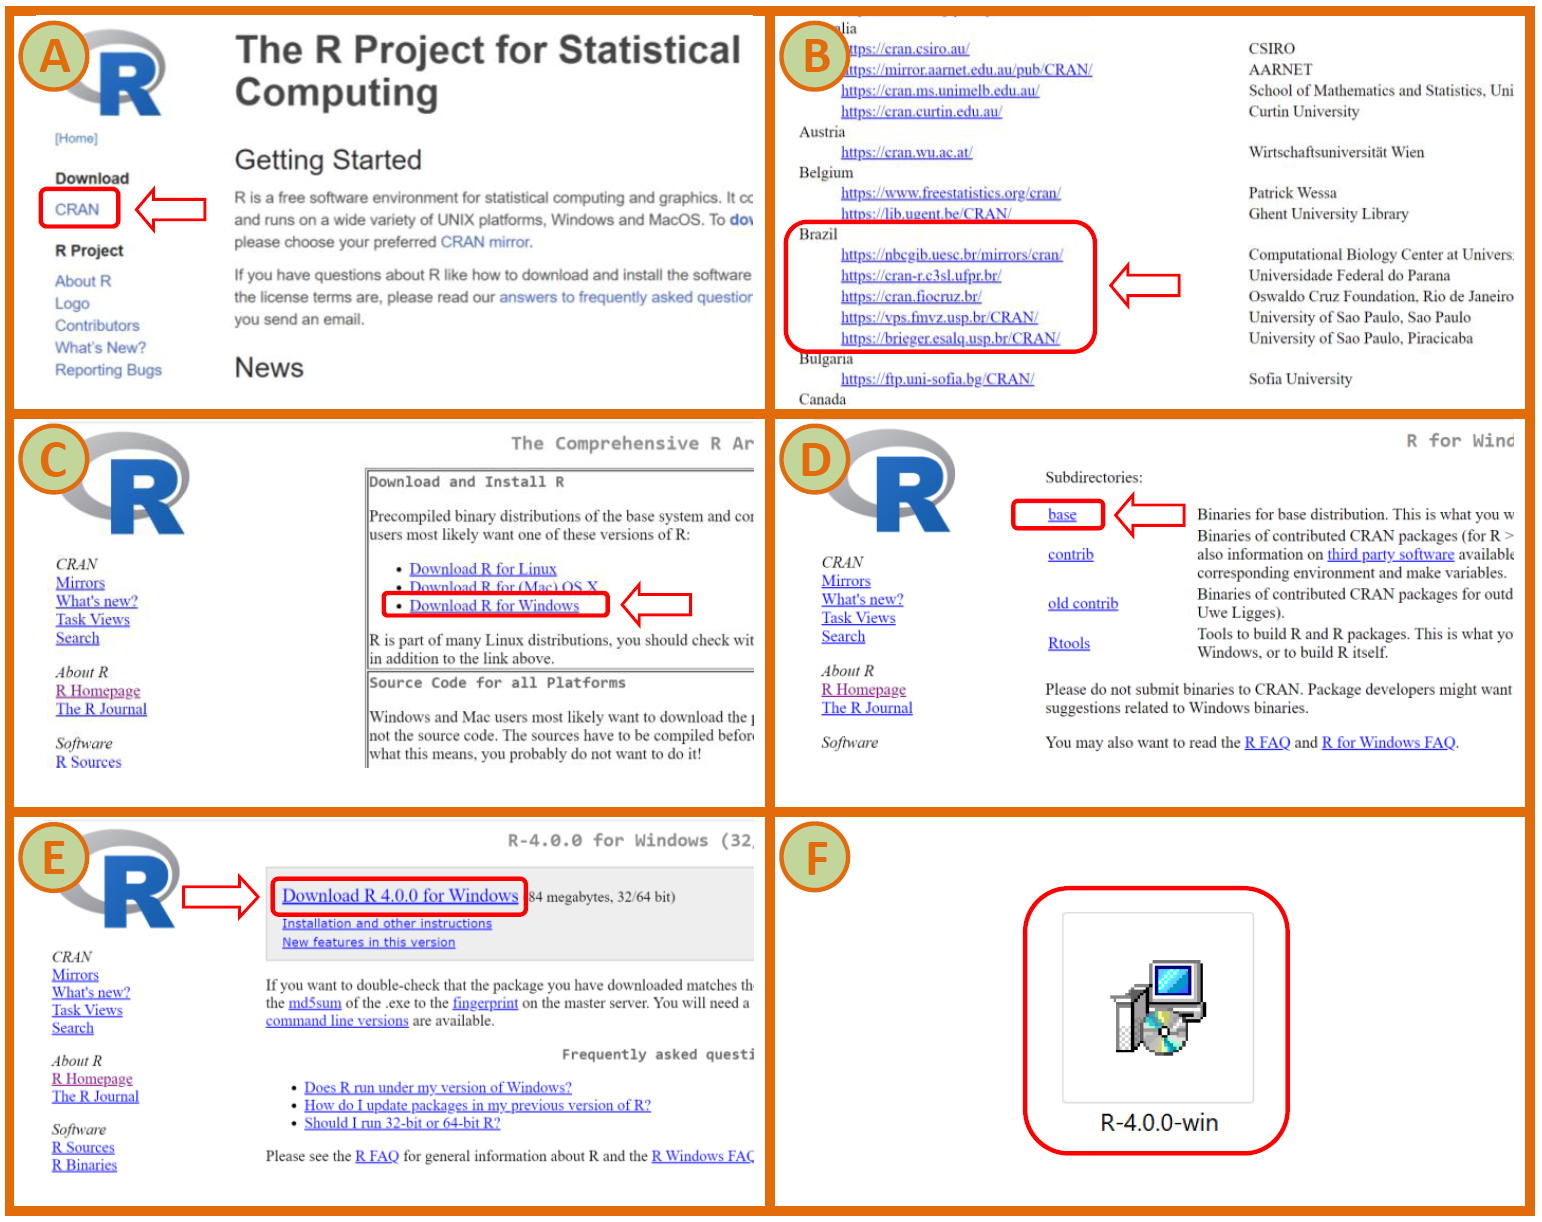
\includegraphics[scale=0.645]{Rdownload.png}
\setlength{\abovecaptionskip}{0.5pt}
\caption{Passos para fazer o download do R}
\label{fig:Rdownload} % Unique label used for referencing the figure in-text
\end{figure}


Após fazer o download do arquivo de instalação do R (Figura~\ref{fig:Rdownload} F) dê um clique duplo sobre ele para executá-lo. Selecione o idioma "Português Brasileiro" (Figura~\ref{fig:Rinstal} A) e clique em "OK". Nas próximas janelas que irão abrir (Figuras~\ref{fig:Rinstal} B à G) basta clicar em "Próximo" para fazer a instalação padrão do R. Por fim clique em "Concluir" (Figura~\ref{fig:Rinstal} H) para finalizar a instalação. 


\begin{figure}[t!]
\centering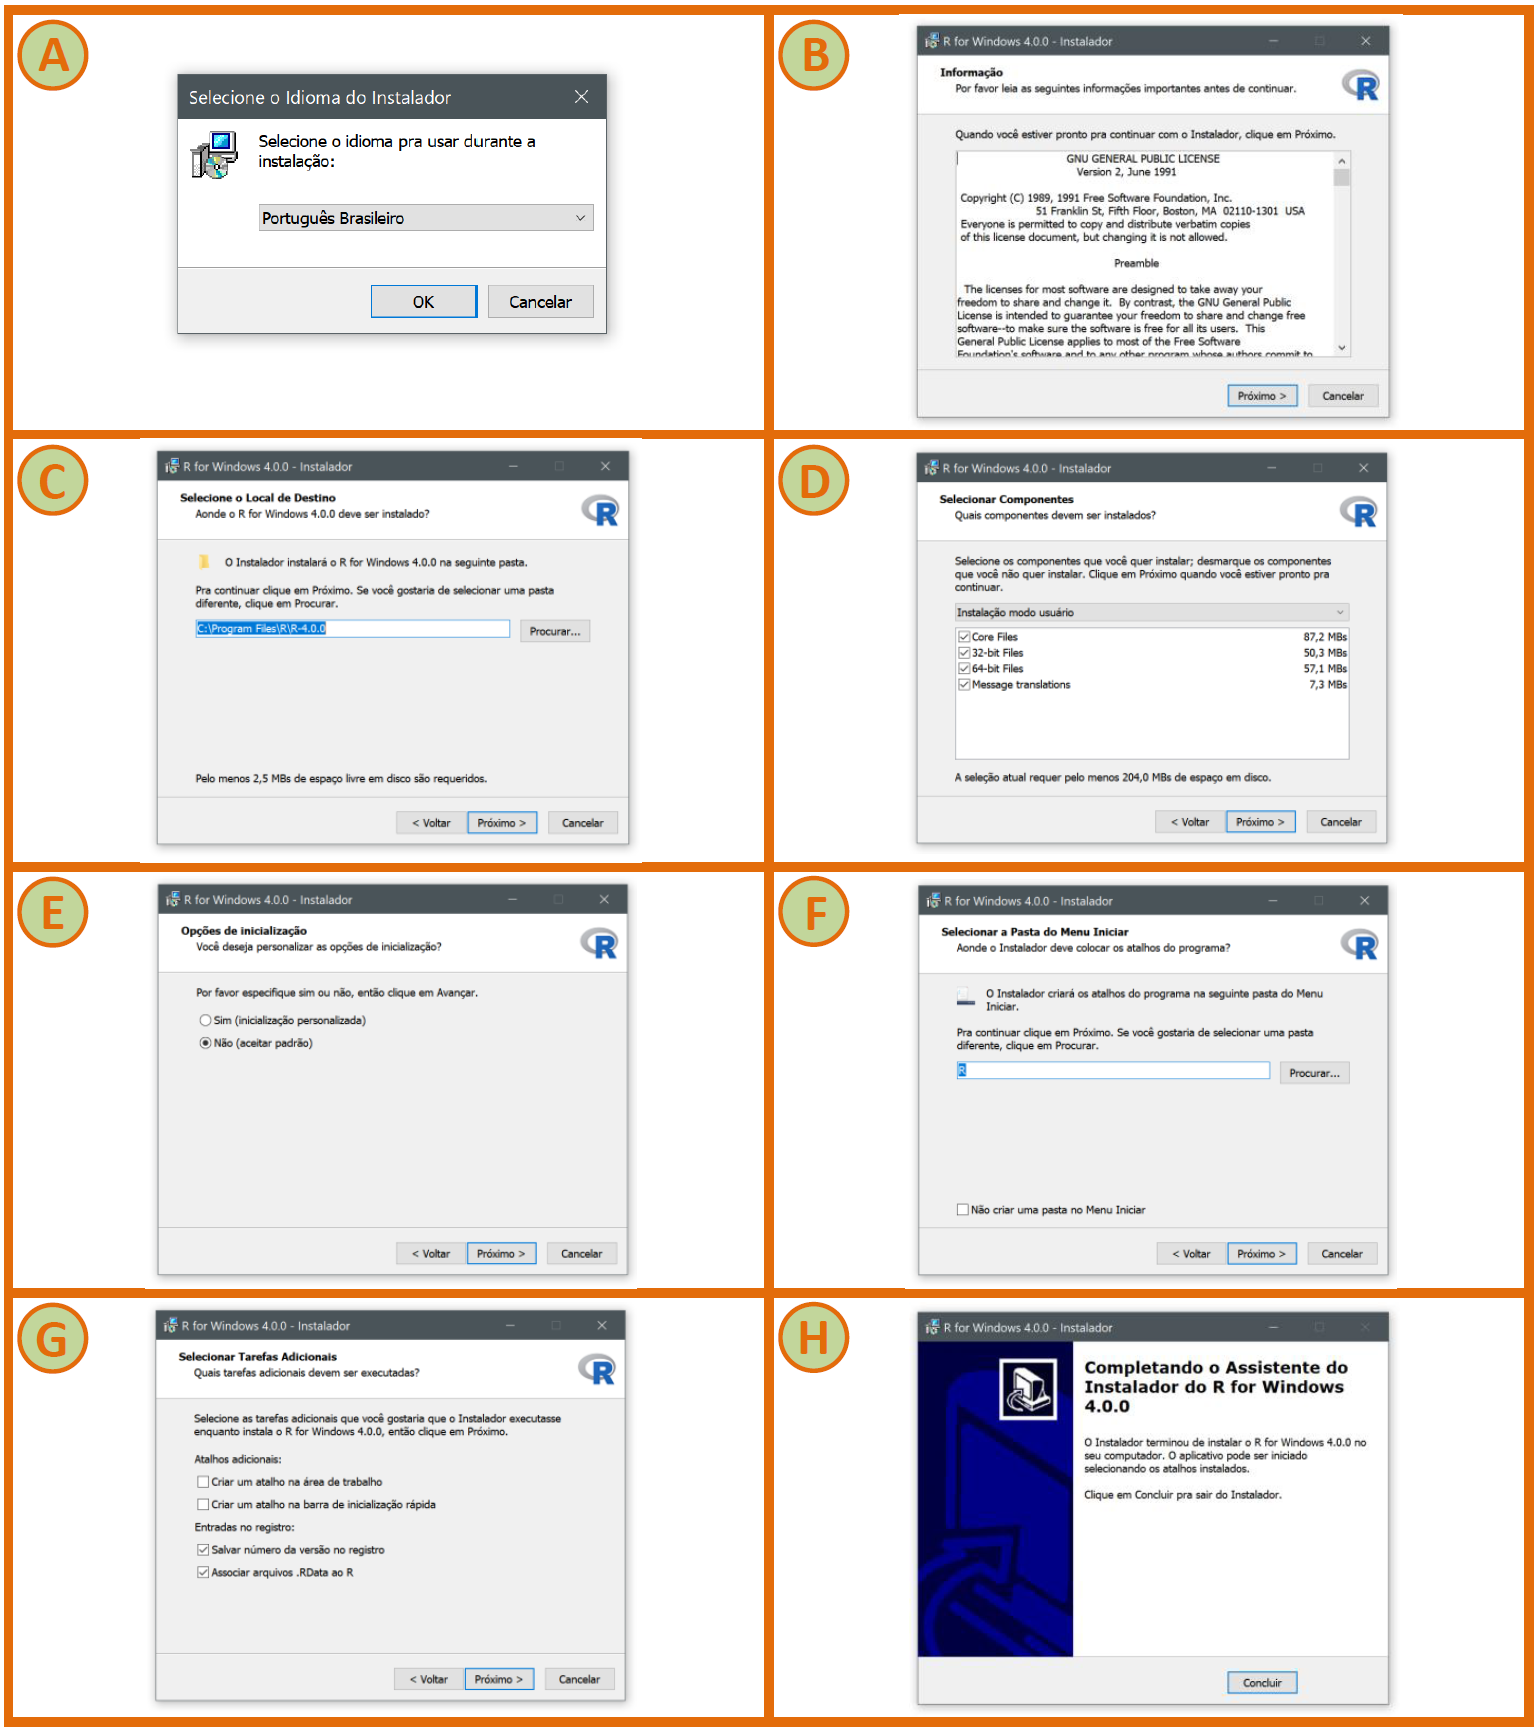
\includegraphics[scale=0.645]{Rinstal.png}
\setlength{\abovecaptionskip}{0.5pt}
\caption{Passos para fazer a instlação do R}
\label{fig:Rinstal} % Unique label used for referencing the figure in-text
\end{figure} 


%Após finalizar a instalação do software R será criado um atalho na área de trabalho com o ícone igual ao da Figura~\ref{fig:Ricone}. Dê um clique duplo sobre o ícone para abrir o software R. 

Após finalizar a instalação será criado um atalho para o software R na área de trabalho. Dê um clique duplo sobre o atalho para executar o R.

%\begin{figure}[h]
%\centering
\includegraphics[scale=1]{Ricone.png}
%\setlength{\abovecaptionskip}{0.5pt}
%\caption{Atalho para executar o software R}
%\label{fig:Ricone} % Unique label used for referencing the figure in-text
%\end{figure}


Na Figura~\ref{fig:Rlayout} pode-se observar a aparência do software R . Ao abrir o programa é mostrado um menu superior e uma janela principal chamada {\itshape R Console}. É nesta janela que os comandos são executados. 


\begin{figure}[t!]
%\centering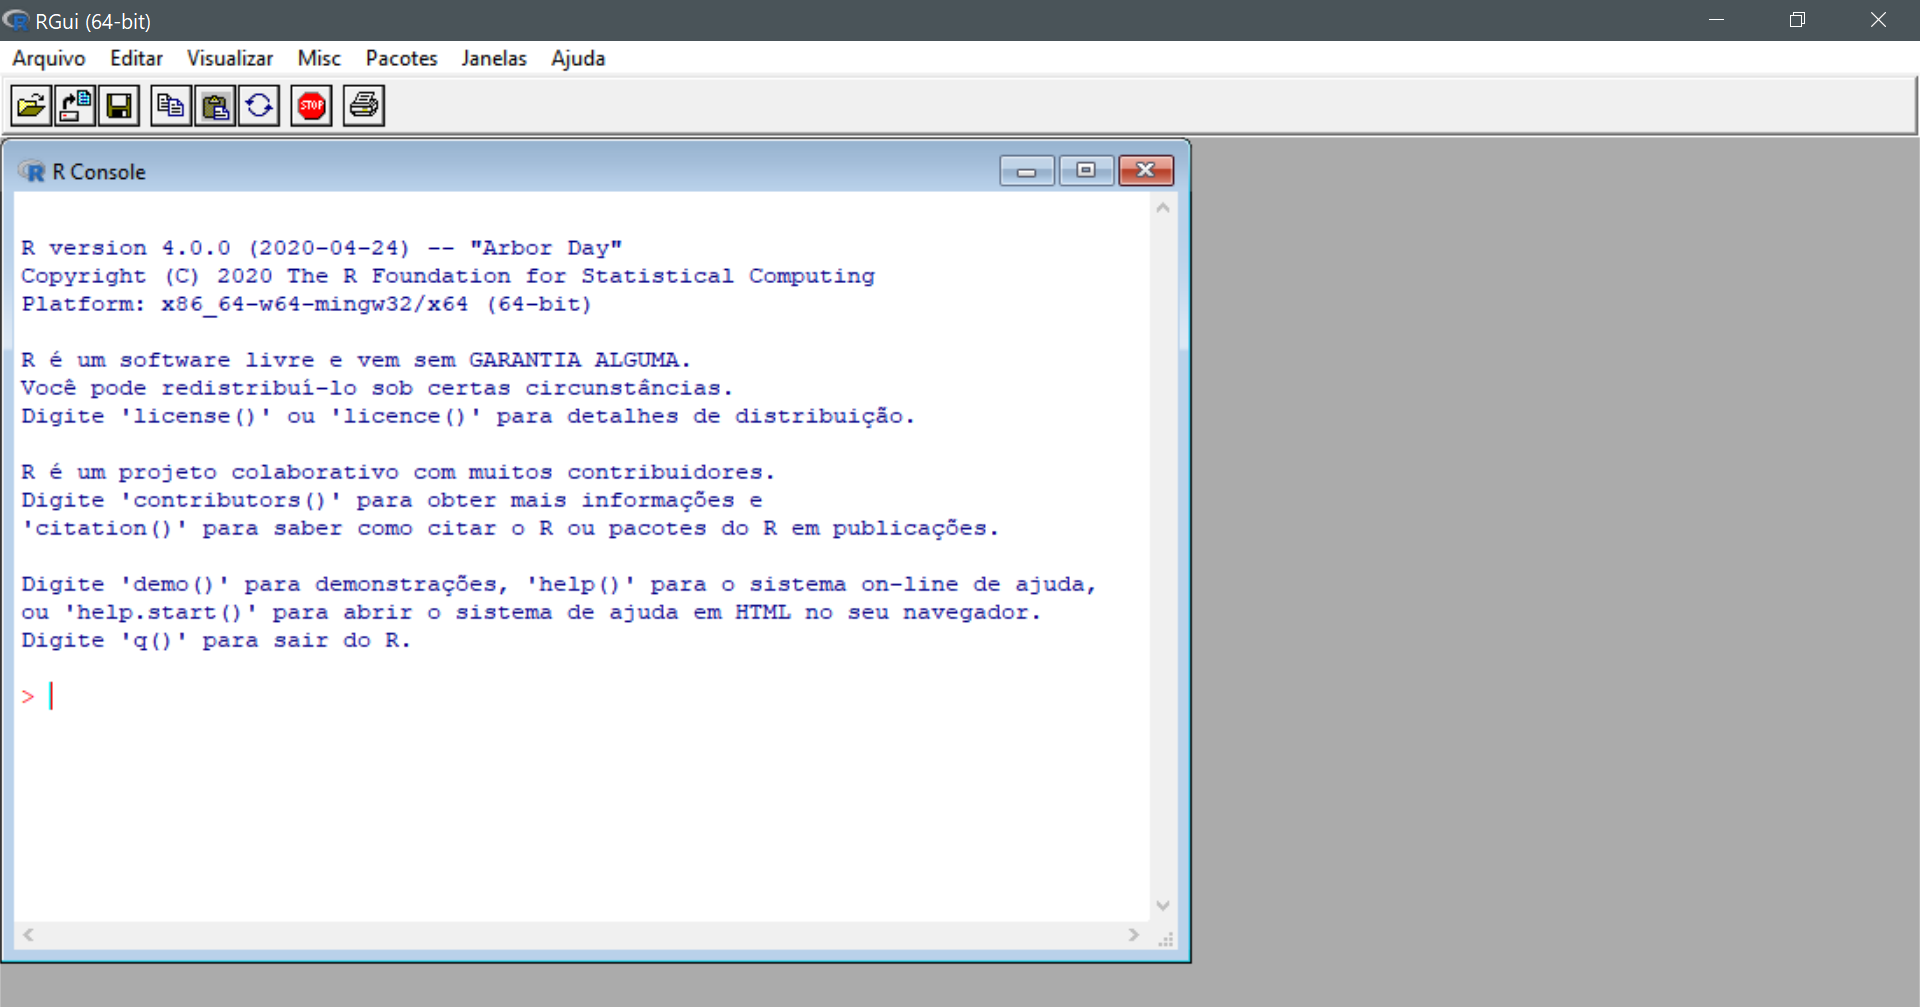
\includegraphics[scale=0.515]{Rlayout.png}
\centering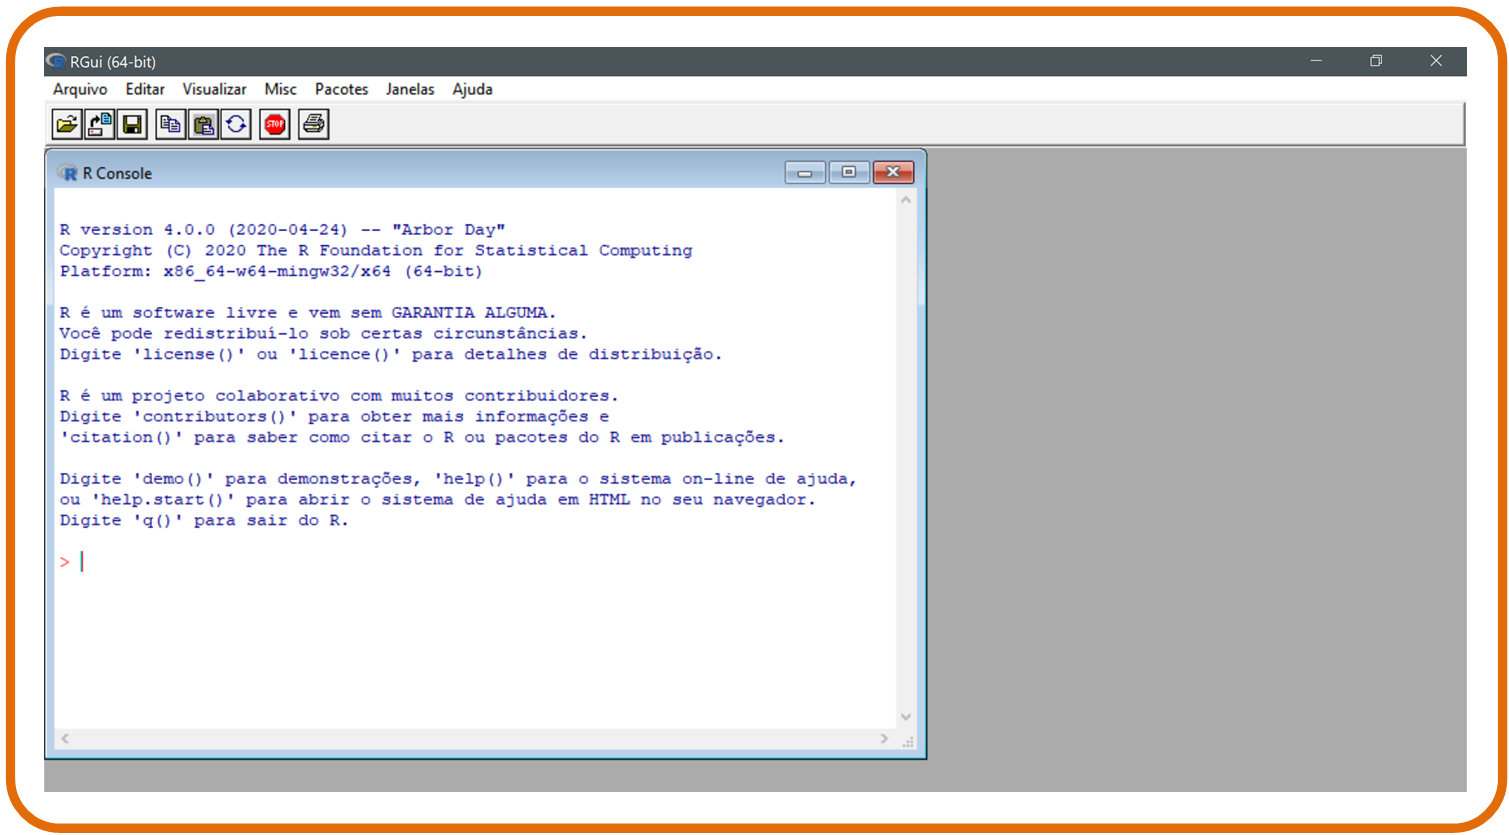
\includegraphics[scale=0.66]{Rlayout2.png}
\setlength{\abovecaptionskip}{0.5pt}
\caption{Aparência do software R}
\label{fig:Rlayout} % Unique label used for referencing the figure in-text
\end{figure}




%----------------------------------------------------------------------------------------
%	CHAPTER 2
%----------------------------------------------------------------------------------------

\chapterimage{chapter_head_4.pdf} % Chapter heading image

\chapter{Download e instalação do RStudio}

%------------------------------------------------

\section{Sobre o RStudio}

O RStudio é um ambiente de desenvolvimento integrado (IDE) para R. Ele inclui um console, editor de realce de sintaxe que suporta execução direta de código, além de ferramentas para plotagem, histórico, depuração e gerenciamento de espaço de trabalho. Basicamente, o RStudio é uma interface gráfica mais prática e otimizada para o R. O software R é executado diretamente a partir do RStudio. 

O RStudio está disponível em edições comerciais e de código aberto e é executado na área de trabalho (Windows, Mac e Linux) ou em um navegador conectado ao RStudio Server ou ao RStudio Server Pro (Debian / Ubuntu, Red Hat / CentOS e SUSE Linux). Maiores informações em \url{https://rstudio.com/about/}.


%------------------------------------------------

\section{Download e instalação do RStudio}

Neste material serão apresentados os passos para download e instalação do RStudio apenas para o sistema operacional Windows. Na Figura~\ref{fig:RSdownload} podemos ver os passos para fazer o download do RStudio. Na página inicial do site do RStudio (Figuras~\ref{fig:RSdownload} A e B) clique em "Download" e você será redirecionado para outra página (Figura~\ref{fig:RSdownload} C). Nesta página desça a barra de rolagem localizada à direita até que apareçam as opções de download gratuitas e pagas (Figura~\ref{fig:RSdownload} D) e clique na opção {\itshape RStudio Desktop Free} (Figura~\ref{fig:RSdownload} E) para que você seja redirecionado para a página de download do RStudio Desktop 1.3.959 (Figuras~\ref{fig:RSdownload} F e G). Nesta página clique em {\itshape DOWNLOAD RSTUDIO FOR WINDOWS} e será feito o download do arquivo de instalação do RStudio (Figura~\ref{fig:RSdownload} H). Até o momento em que este material foi elaborado a versão mais recente do RStudio era a 1.3.959.



\begin{figure}[t!]
\centering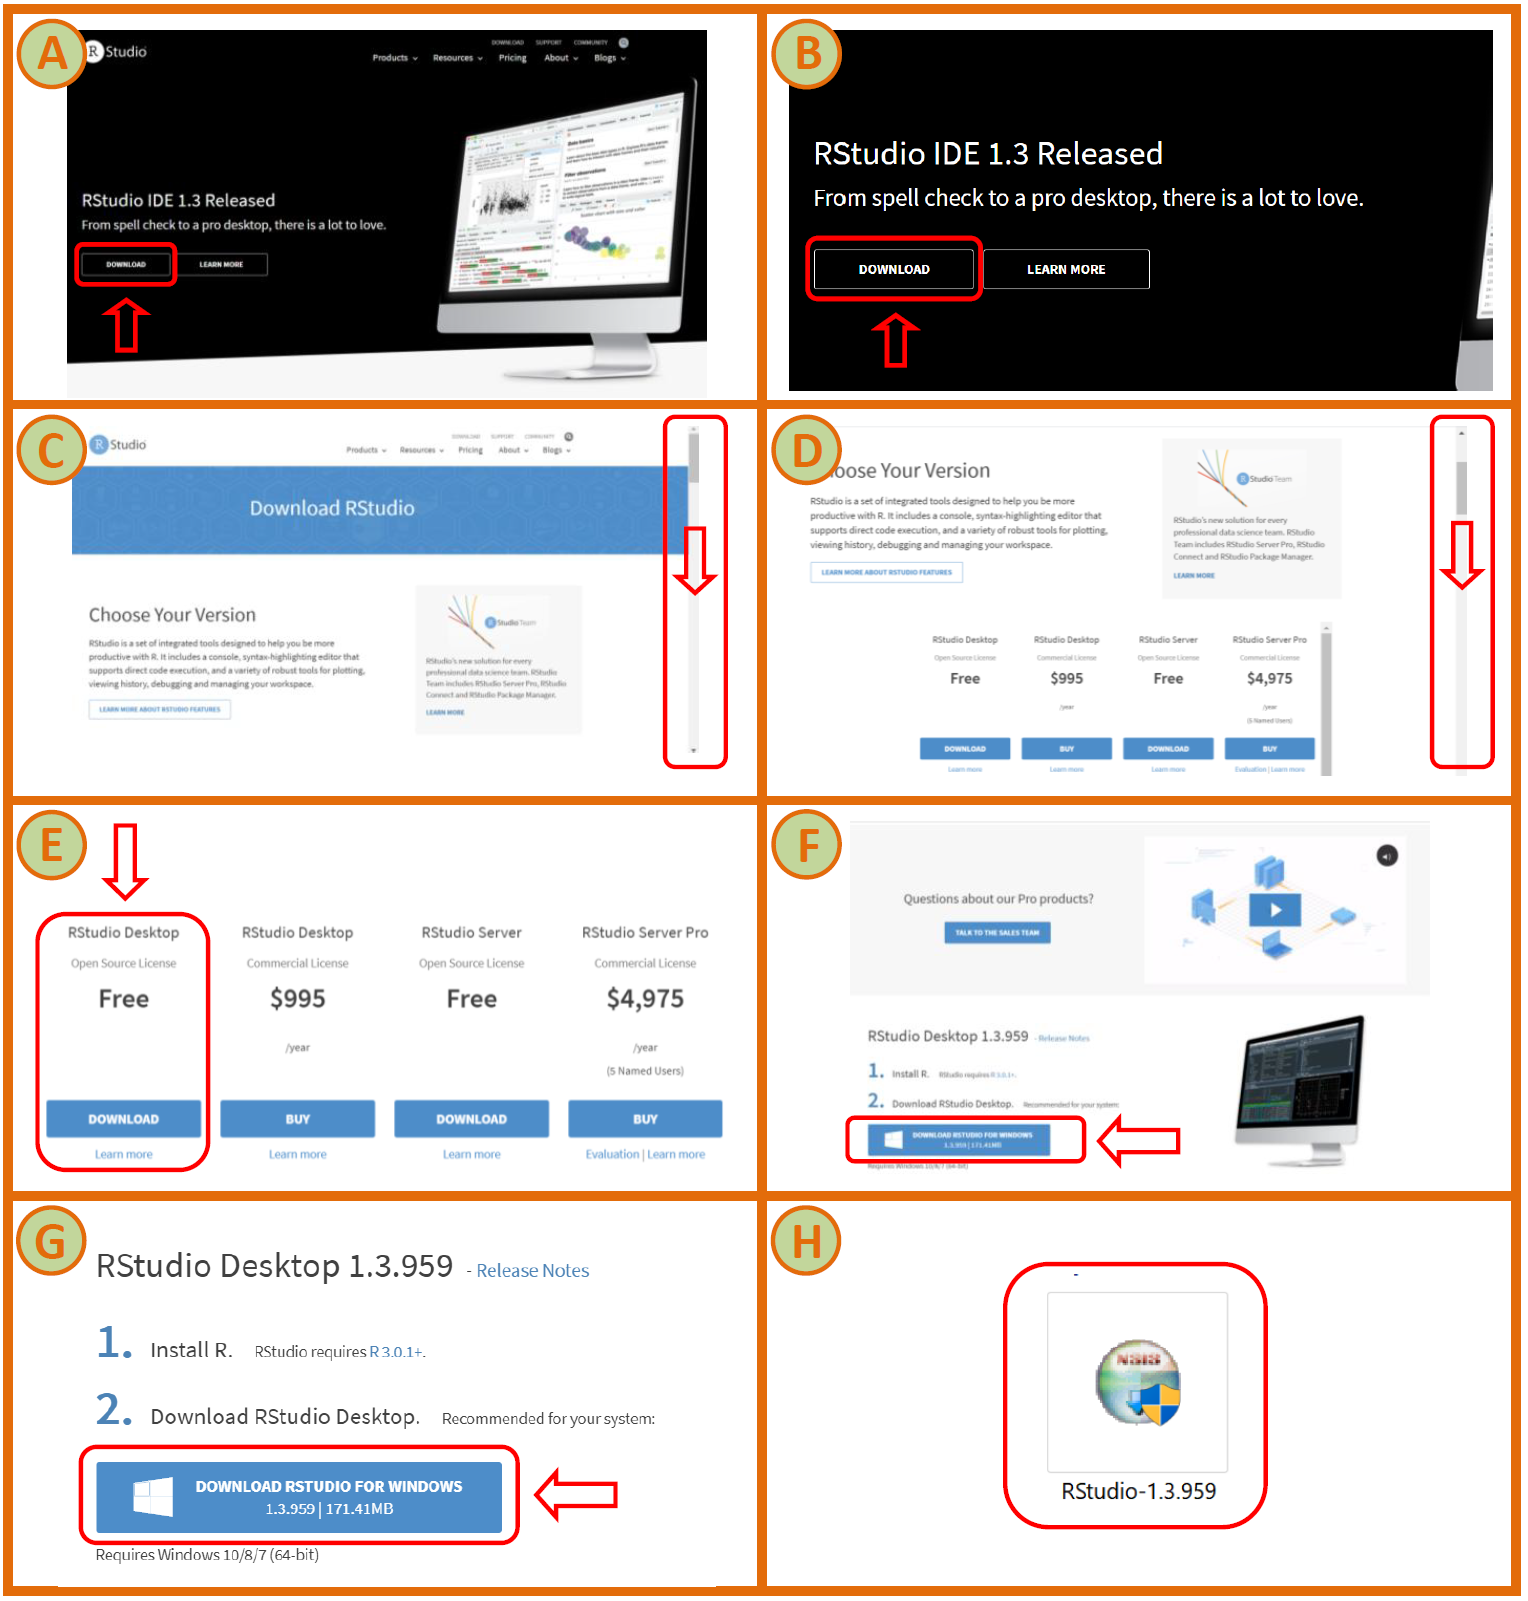
\includegraphics[scale=0.65]{RSdownload.png}
\setlength{\abovecaptionskip}{0.5pt}
\caption{Passos para fazer o download do RStudio}
\label{fig:RSdownload} % Unique label used for referencing the figure in-text
\end{figure}


Após fazer o download do arquivo de instalação do RStudio (Figura~\ref{fig:RSdownload} H) dê um clique duplo sobre ele para executá-lo. Nas janelas que irão abrir (Figuras~\ref{fig:RSinstal} A à C) basta clicar em "Próximo" para fazer a instalação padrão do RStudio. Por fim clique em "Concluir" (Figura~\ref{fig:RSinstal} D) para finalizar a instalação. 


\begin{figure}[h]
\centering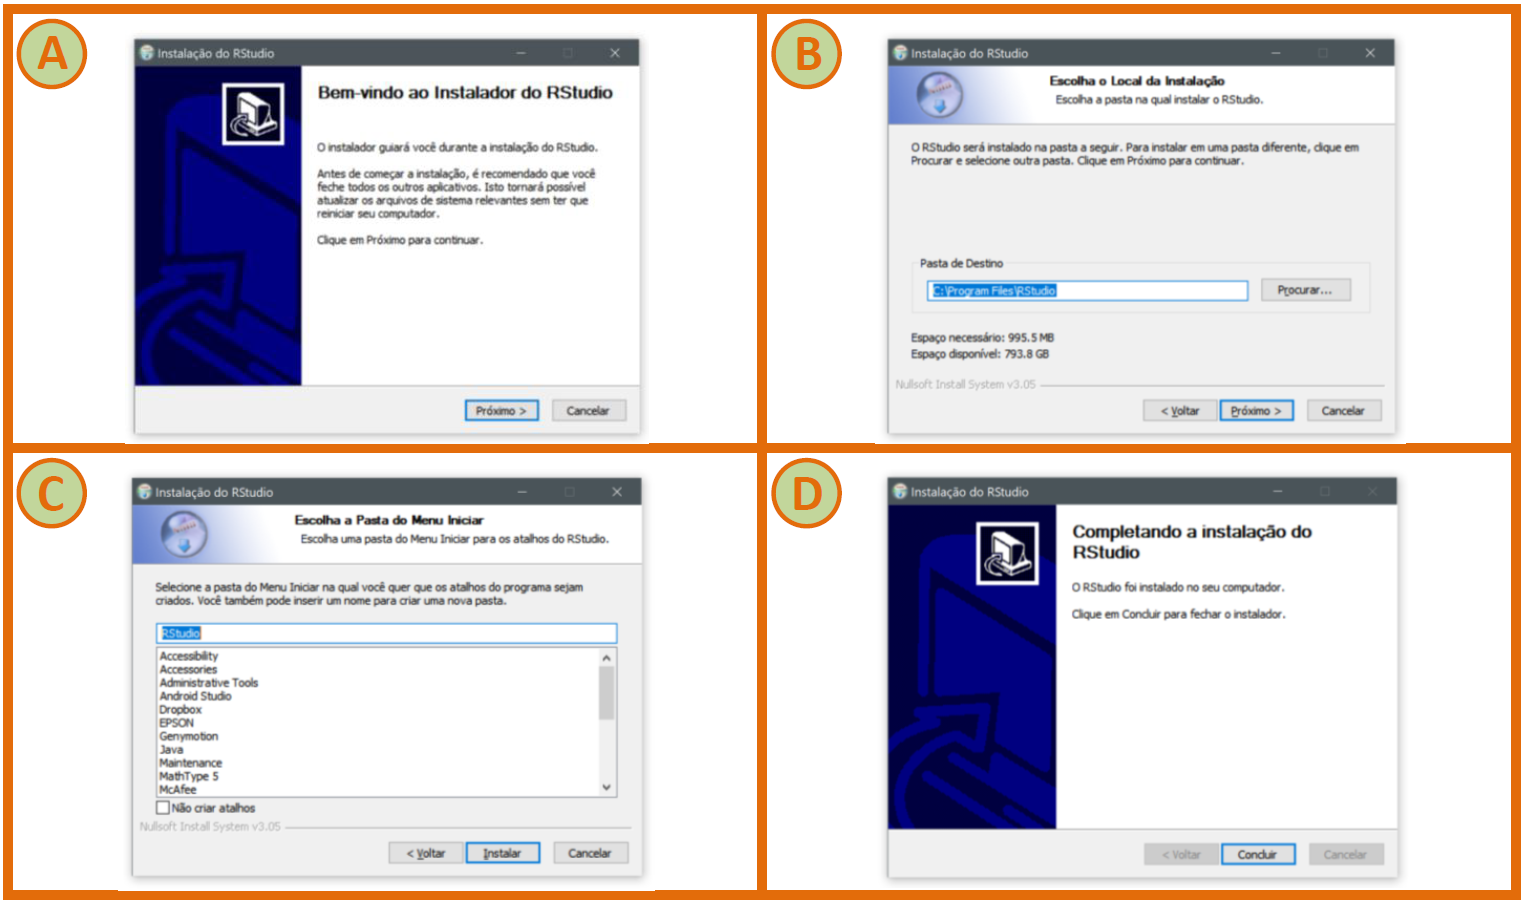
\includegraphics[scale=0.65]{RSinstal.png}
\setlength{\abovecaptionskip}{0.5pt}
\caption{Passos para fazer a instalação do RStudio}
\label{fig:RSinstal} % Unique label used for referencing the figure in-text
\end{figure}


%Após finalizar a instalação do RStudio será criado um atalho na área de trabalho com o ícone igual ao da Figura~\ref{fig:RSicone}. Dê um clique duplo sobre o ícone para abrir o RStudio. \\ \\ \\


%\begin{figure}[h]
%\centering
\includegraphics[scale=1.1]{RSicone.png}
%\setlength{\abovecaptionskip}{0.5pt}
%\caption{Atalho para executar o RStudio}
%\label{fig:RSicone} % Unique label used for referencing the figure in-text
%\end{figure}


Após finalizar a instalação será criado um atalho para o RStudio na área de trabalho. Dê um clique duplo sobre o atalho para executar o RStudio. 


Na Figura~\ref{fig:RSlayout} pode-se observar a aparência do RStudio. Ao abrir o programa é mostrado um menu superior e quatro janelas. A janela superior esquerda é a janela do {\itshape Script}, a janela inferior esquerda é a janela do {\itshape Console}, a janela superior direita é responsável principalmente por listar os objetos gerados e a janela inferior direita é responsável principalmente por exibir os gráficos gerados. Caso não apareça a janela do {\itshape Script} na primeira seção do RStudio, você pode criar um script acessando o menu superior em {\bf File \texttt{->} New File \texttt{->} R Script}.


\begin{figure}[h]
%\centering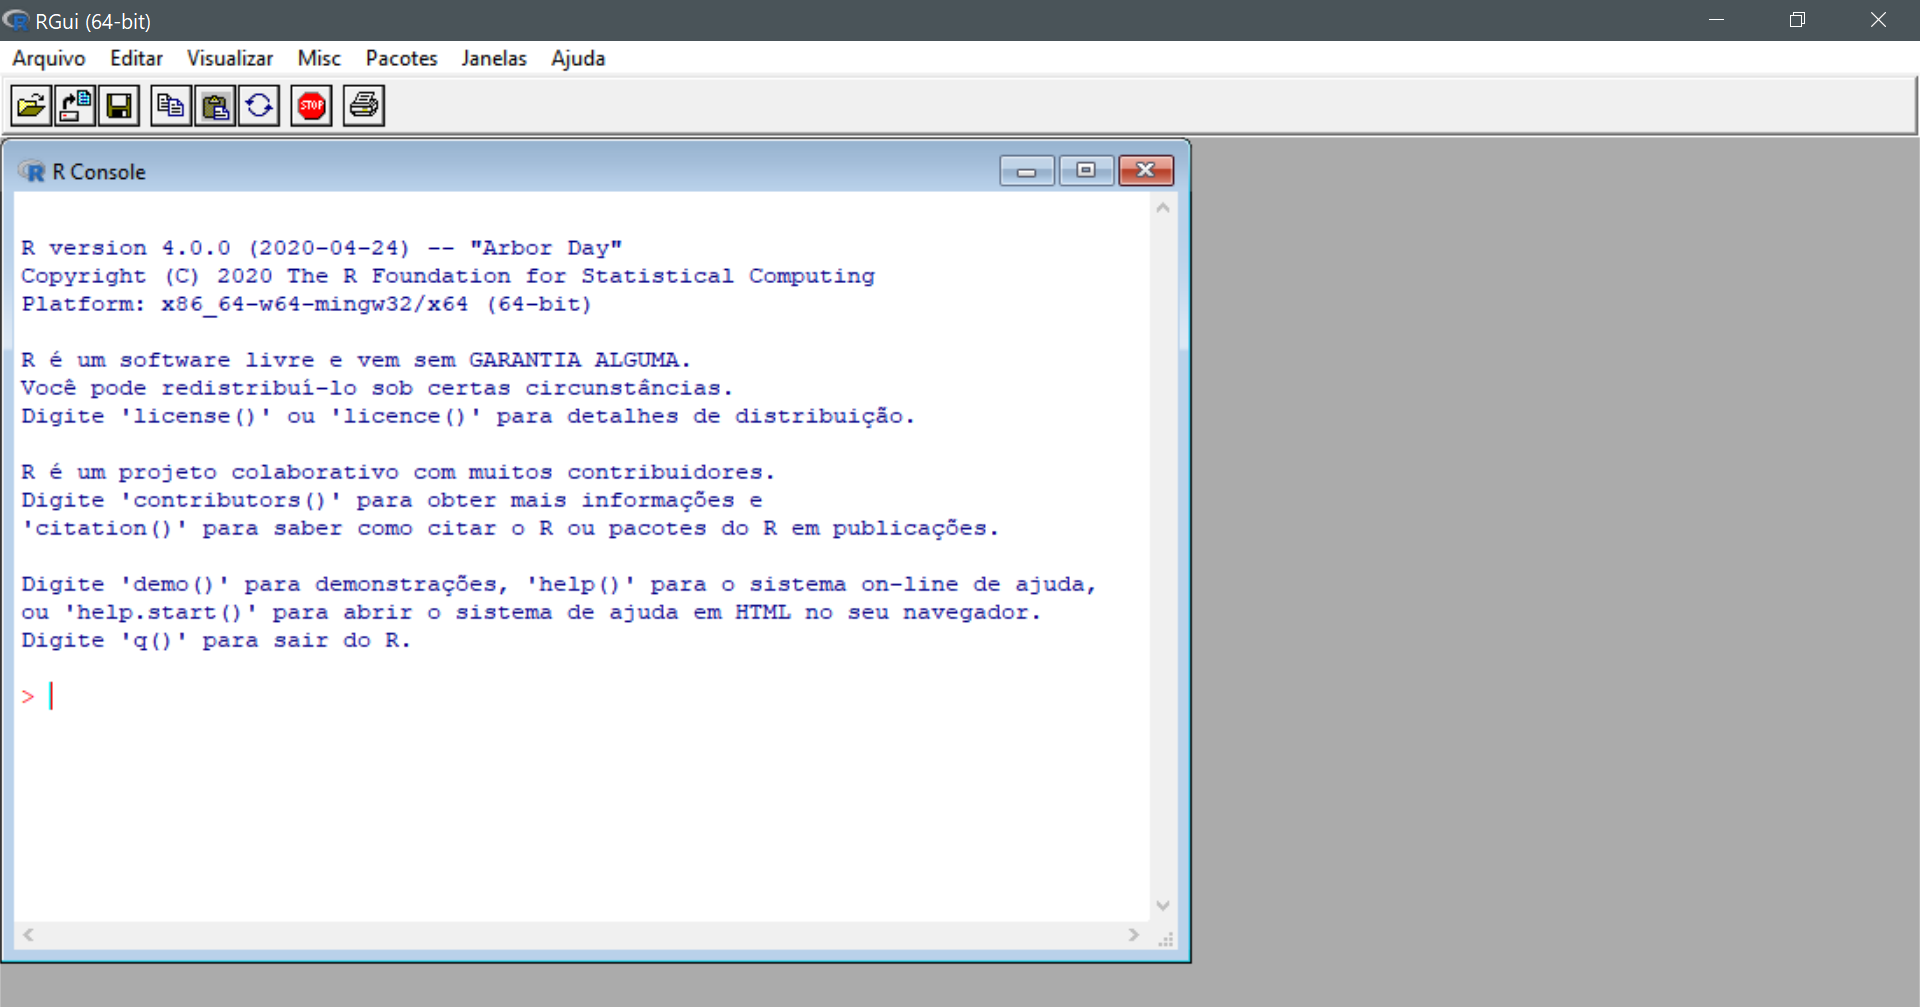
\includegraphics[scale=0.515]{Rlayout.png}
\centering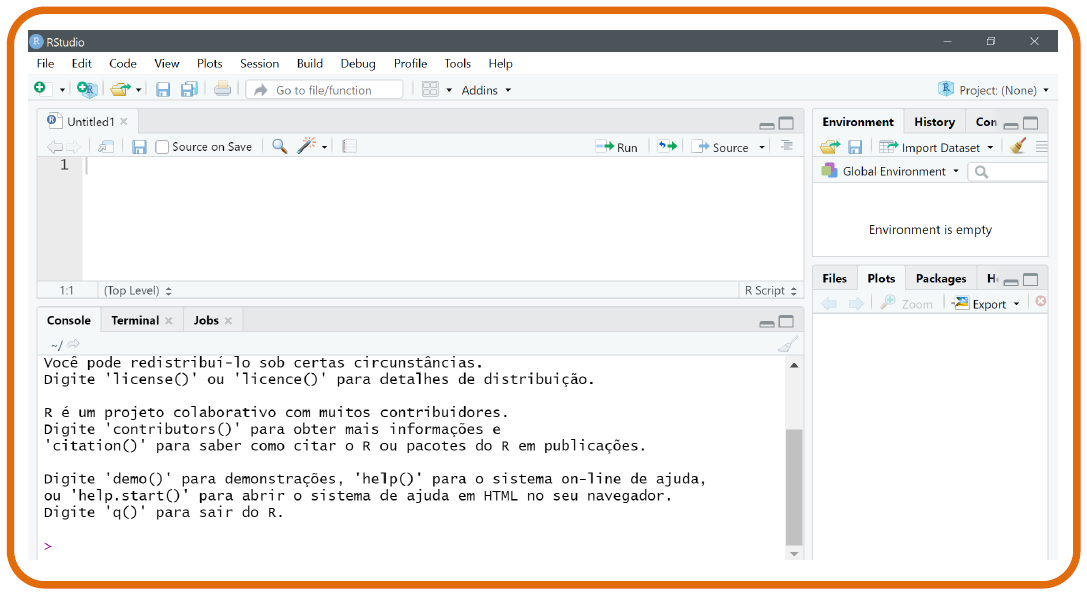
\includegraphics[scale=0.92]{RSlayout.png}
\setlength{\abovecaptionskip}{0.5pt}
\caption{Aparência do RStudio}
\label{fig:RSlayout} % Unique label used for referencing the figure in-text
\end{figure}


%----------------------------------------------------------------------------------------
%	CHAPTER 3
%----------------------------------------------------------------------------------------

\chapterimage{chapter_head_2.pdf} % Chapter heading image

\chapter{Introdução ao Software R}

%------------------------------------------------

\section{Console}

A janela principal do R, que é iniciada junto com o programa é chamada de {\itshape R Console}. É nesta janela que os comandos digitados são executados. Para executar um comando no console basta digitar o comando e pressionar a tecla \texttt{ "Enter"}. Na Figura~\ref{fig:Rlayoutll} a janela do console é a janela localizada no lado direito enquanto a janela localizada no lado esquerdo é chamada de {\itshape Script}.


\section{Script}

Uma desvantagem de se digitar os comandos diretamente no console é que depois de executar uma linha de comando não se pode editá-la nesta janela e fica difícil escrever e salvar todos os comandos de forma organizada. 

Ao invés de digitar os comandos do R diretamente no console pode-se abrir uma nova janela no R chamada de {\itshape Script}. Nesta janela os comandos podem ser digitados e editados sem que eles sejam automaticamente executados, e, para que uma linha de comando do script seja enviada para o console e executada deve-se posicionar o cursor sobre a linha de comando do script e depois pressionar as teclas \texttt{"Ctrl"} e \texttt{"R"} juntas. 

Na Figura~\ref{fig:Rlayoutll} a janela localizada no lado esquerdo, inicalmente nomeada como {\itshape "Sem nome - Editor R"} (pelo fato de ainda não ter sido salva) é um script. Após salvar o script pode-se escolher um outro nome para ele.

Para abrir um novo script basta acessar o menu superior do R em: {\bf Arquivo \texttt{->} Novo script}. Para salvar o script, contendo os comandos do R, a janela do script deve estar em uso (para isso basta clicar com o cursor sobre a janela do script) e depois deve-se acessar o menu superior do R em: {\bf Arquivo \texttt{->} Salvar}.

Pode-se organizar as janelas do R (script e console) de forma que elas fiquem divididas lado à lado, como na Figura~\ref{fig:Rlayoutll}, ou ainda, divididas na horizontal. Para isso, basta acessar o menu superior do R em {\bf \texttt{Janelas -> Dividir Lado a Lado}} ou, ainda, {\bf \texttt{Janelas -> Dividir na Horizontal}}.

\begin{figure}[h]
%\centering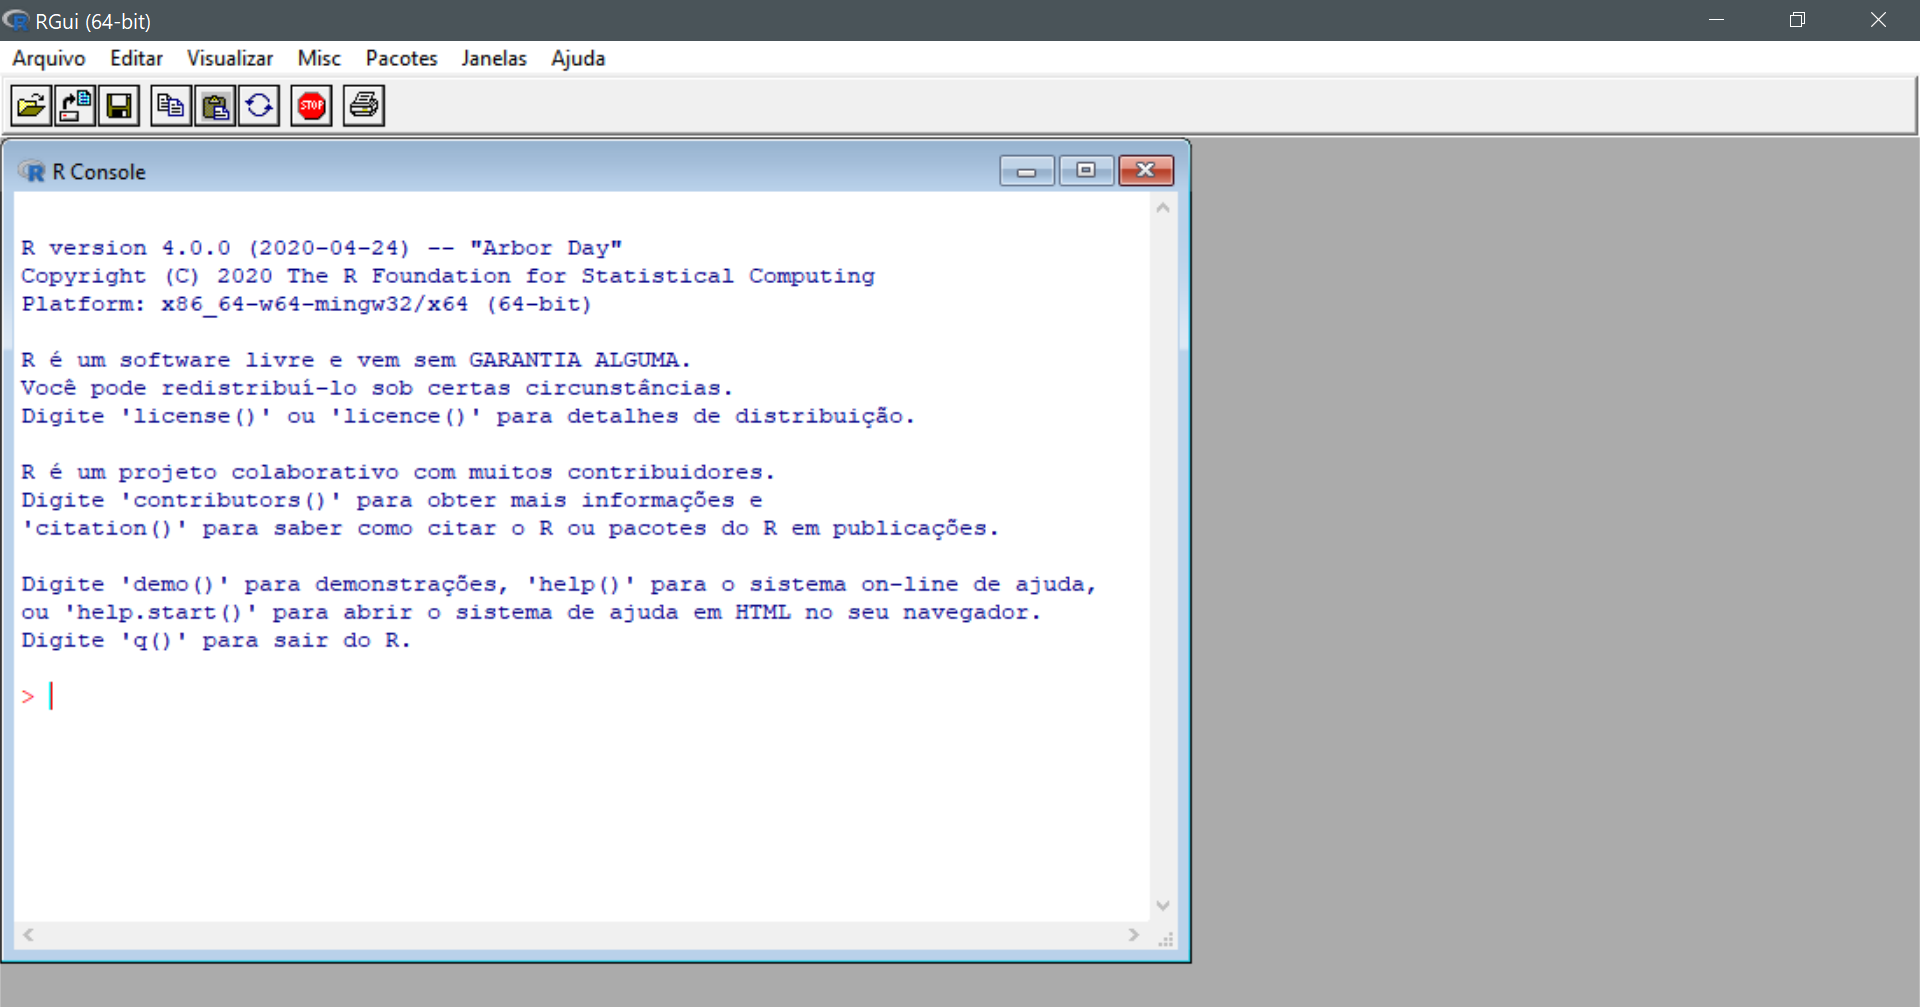
\includegraphics[scale=0.515]{Rlayout.png}
\centering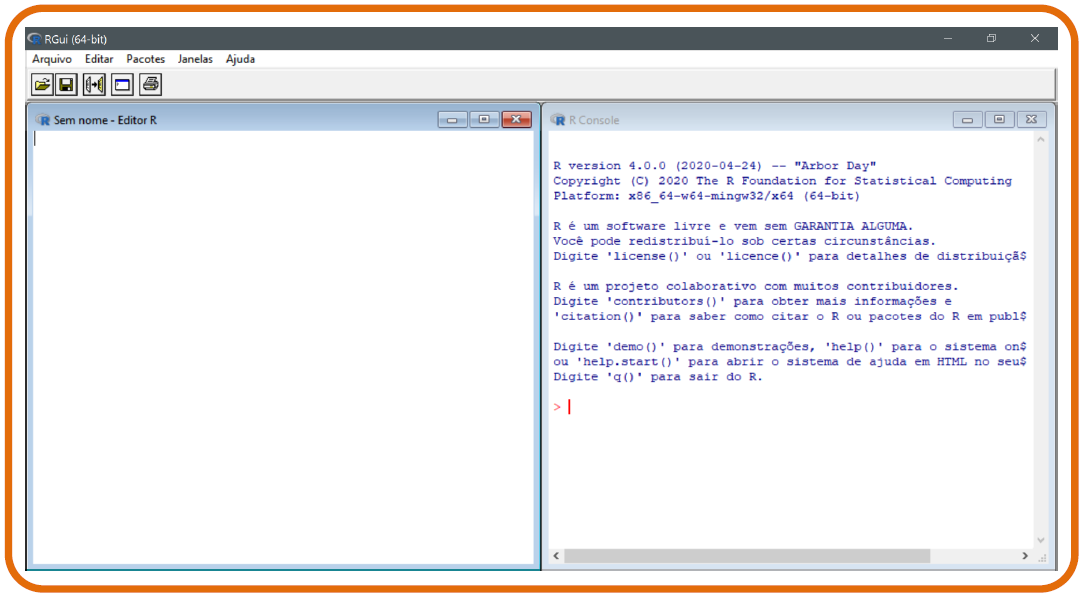
\includegraphics[scale=0.923]{Rlayoutll.png}
\setlength{\abovecaptionskip}{0.5pt}
\caption{Software R com janelas divididas lado à lado}
\label{fig:Rlayoutll} % Unique label used for referencing the figure in-text
\end{figure}

No RStudio também são usados scripts para digitar e editar os comandos. Você pode criar um script no RStudio acessando o menu superior em {\bf File \texttt{->} New File \texttt{->} R Script}. Para que uma linha de comando do script do RStudio seja enviada para o console e executada deve-se posicionar o cursor sobre a linha de comando do script e depois pressionar as teclas \texttt{"Ctrl"} e \texttt{"Enter"} juntas. Para salvar o script basta acessar o menu superior em {\bf File \texttt{->} Save As...}.


\section{Pacotes}

Um elemento fundamental na estrutura do software R está relacionado com os comandos de execução de operações e técnicas, denominado de funções. As funções são disponibilizadas no R através de pacotes  {\itshape (package)}, também chamados de bibliotecas  {\itshape (library)}.

Os comandos básicos (funções básicas) já vem pré instalados e se encontram no pacote  {\itshape base}. Há uma considerável oferta de pacotes com conteúdos diversos desenvolvidos por colacoradores. Para acessá-los é preciso realizar a instalação do pacote de interesse no R, pois diferente do pacote  {\itshape base}, os demais pacotes não são disponibilizados na instalação do R.

A instalação de um pacote é realizada com o uso do comando \texttt{install.packages()}. Uma vez que o pacote é instalado deve-se fazer o seu carregamento na memória do programa, toda vez que se inciar uma nova seção do R, com o uso do comando \texttt{library()}. Na Lista~\ref{lst:Rintro1} são apresentados os comandos do software R para fazer a instalação e carregamento de um pacote (neste exemplo foi usado o pacote \texttt{agricolae}). Após o carregamento do pacote \texttt{agricolae}, todas as funções que compõem este pacote podem ser utilizadas pelo usuário. \\


\begin{scriptsize}
	\estiloR
	\begin{lstlisting}[caption={Comandos do software R}, label=lst:Rintro1]
	# Instalação do pacote agricolae
	install.packages("agricolae")
	
	# Carregamento do pacote agricolae
	library("agricolae")
	
	\end{lstlisting}
\end{scriptsize}


%------------------------------------------------

\section{Operações matemáticas básicas}

Na Lista~\ref{lst:Rintro2} são apresentados os comandos do software R para calcular alguns elementos de matemática básica. \\

\begin{scriptsize}
	\estiloR
	\begin{lstlisting}[caption={Comandos do software R}, label=lst:Rintro2]
	# Adição
	5+3
	
	# Subtração
	5-3
	
	# Multiplicação
	5*3	
	
	# Divisão
	5/3
	
	# Potenciação
	5^3	
	
	# Raiz quadrada
	sqrt(100)
	
	# Exponencial
	exp(0)
	exp(1)	
	
	# Logarítmo na base e
	log(1)
	log(2)
	
	# Logarítmo na base 10
	log10(1)
	log10(2)
	
	\end{lstlisting}
\end{scriptsize}


%------------------------------------------------

\section{Armazenamento de dados}

Os tipos de dados mais comumente utilizados no R são os numéricos (dados compostos por números) e os caracteres (compostos por letras ou palavras). As informações imputadas no R são armazenadas na memória do programa e passam a ser denominadas {\itshape objetos}. Para criar um objeto basta associar um nome à informação de interesse, e, para isso, utiliza-se o símbolo \, {\bf \texttt{<--}} \, ou \, {\bf \texttt{=}} \, entre o nome do objeto e a informação que define o objeto. No caso de objeto formado por caracteres a informação armazenada deve vir entre aspas.

Na Lista~\ref{lst:Rintro3} são apresentados os comandos do software R para fazer a entrada de dados numéricos e de caracteres. Observe, no último comando da lista, que pode-se usar o \texttt{";"} para colocar dois comandos diferentes (criar o objeto e mostrar o objeto) em uma mesma linha. \\


\begin{scriptsize}
	\estiloR
	\begin{lstlisting}[caption={Comandos do software R}, label=lst:Rintro3]
	# Entrando com um dado numérico (criando o objeto x)
	x <- 10
	
	# Mostrando o objeto x
	x
		
	# Entrando com um dado de caracteres (criando o objeto y)
	# e mostrando o objeto (comandos na mesma linha separados por ";")
	y <- "bola" ; y
	
	\end{lstlisting}
\end{scriptsize}


Algumas regras devem ser seguidas na hora de nomear um objeto. O nome do objeto precisa começar com uma letra, não pode ser um número, não pode conter símbolos referentes a funções ou nome de funções e a "seta" \, {\bf \texttt{<--}} \, deve estar sempre apontada para o nome do objeto. \\

{\bf Observação}: O R diferencia letras maiúsculas e minúsculas. Assim, por exemplo, ao criar um objeto "x" (minúsculo) deve-se sempre se referir a ele com a letra x minúscula pois, se for utilizada a letra X (maiúscula) o R irá retornar uma mensagem de erro: "\texttt{Erro: objeto 'X' não encontrado}".\\


%------------------------------------------------
\section{Operadores lógicos}

Na Tabela~\ref{tab:oplog} são apresentados alguns operadores lógicos que são usados para realização de "testes" entre dois objetos.

\begin{table}[h]
	\caption{Operadores lógico}
	\label{tab:oplog} 
	\vspace{0.1cm}
	\centering
	\begin{tabular}{l l}
	\toprule
	\textbf{Operador} & \textbf{Descrição}\\
	\midrule
	\texttt{==} 	& igual a \\
	\texttt{!=} 	& diferente de \\
	\texttt{<}  	& menor que \\
	\texttt{>}  	& maior que \\
	\texttt{<=} 	& menor ou igual a \\
	\texttt{>=} 	& maior ou igual a \\
	\texttt{x | y}	& x OU y \\
	\texttt{x \& y}  & x E y\\
	\bottomrule
	\end{tabular} \\
\end{table}

Na Lista~\ref{lst:Rintro3.2} são apresentados alguns exemplos de comandos do software R utilizando os operadores lógicos apresentados na Tabela~\ref{tab:oplog}. \\

\begin{scriptsize}
	\estiloR
	\begin{lstlisting}[caption={Comandos do software R}, label=lst:Rintro3.2]
	# Criando objetos x e y
	x <- c(1,3,2,4,5,3,2,4); x
	y <- c(1,2,3,4,5,6,7,8); y
	
	# Operador "igual a"
	x==3 
	
	# Operador "diferente de"
	x!=3
	
	# Operador "maior que"
	x>3 
	
	# Operador "maior ou igual a"
	x>=3 
	
	# Operador "OU"
	if(x[2] | y[2] > 2) print("sim") else print("não")
	
	# Operador "E"	
	if(x[2] & y[2] > 2) print("sim") else print("não")
	
	\end{lstlisting}
\end{scriptsize}

Ao executar os comandos das linhas 6, 9, 12 e 15 da Lista~\ref{lst:Rintro3.2} o R irá verificar quais elementos do objeto \texttt{x} satisfazem as condição impostas e retonará \texttt{TRUE} se o elemento satisfaz a condição e \texttt{FALSE} se não satisfaz. O comando da linha 18 irá verificar se o segundo elemento do objeto \texttt{x} {\bf OU} o segundo elemento do objeto \texttt{y} é maior do que o número 2, se sim retornará \texttt{"sim"} e se não retornará \texttt{"não"}, ou seja, se um elemento ou outro for maior que 2 o R retornará \texttt{"sim"}. Já o comando da linha 21 irá verificar se o segundo elemento do objeto \texttt{x} {\bf E} o segundo elemento do objeto \texttt{y} são maiores do que o número 2, se sim retornará \texttt{"sim"} e se não retornará \texttt{"não"}, ou seja, apenas se os dois elementos forem maiores que 2 o R retornará \texttt{"sim"}.


%------------------------------------------------

\section{Arquivos do R}

O R utiliza um diretório (pasta) do computador para gravar, ler, importar e exportar arquivos. Para saber o diretório em uso digite o comando: \texttt{getwd()}. Para alterar o diretório de trabalho digite: \texttt{setwd("C:/Endereço")}. Os principais tipos específicos de arquivos do R são: o \texttt{*.RData} e o \texttt{*.Rhistory}. \\

O arquivo com extensão \texttt{*.RData} representa a área de trabalho na qual são salvos os objetos criados durante uma seção do R. Para salvar uma área de trbalho basta acessar o menu superior do R em: {\bf Arquivo \texttt{->} Salvar área de trabalho...} \\

O arquivo com extensão \texttt{*.Rhistory}, denominado de histórico, armazena todos os comandos utilizados em uma seção R. Os arquivos de histórico apresentam o formato de texto e por isso podem ser visualizados como um arquivo \texttt{*.txt}. Para salvar um histórico basta acessar o menu superior do R em: {\bf Arquivo \texttt{->} Salvar Histórico...} \\

Um Script é uma janela onde os comandos do R podem ser digitados e editados sem que sejam executados. Para abrir um novo script basta acessar o menu superior do R em: {\bf Arquivo \texttt{->} Novo script}. Para salvar o script contendo os comandos do R basta clicar sobre a janela do script e depois acessar o menu superior do R em: {\bf Arquivo \texttt{->} Salvar}. Os scripts apresentam o formato de texto e por isso podem ser visualizados como um arquivo \texttt{*.txt}. Caso o R esteja em uso a partir do RStudio basta salvar o script para que os comandos utilizados sejam salvos.


%------------------------------------------------

\section{Estrutura de dados}

No R, os dados contidos em um objeto podem assumir distintas estruturas. As mais utilizadas são os vetores, as matrizes e os data-frames.	


\subsection{Vetores}

Um vetor é a forma mais simples de armazenamento de dados. Pode ser um vetor numérico ou de caracteres. A função \texttt{c()} é utilizada na criação do vetor. Na Lista~\ref{lst:Rintro4} são apresentados os comandos do software R para criar um vetor numérico e um vetor de caracteres. \\

\begin{scriptsize}
	\estiloR
	\begin{lstlisting}[caption={Comandos do software R}, label=lst:Rintro4]
	# Vetor com dados numéricos
	x <- c(10, 20, 30)
	
	# Mostrando o vetor x
	x
	
	# Vetor de caracteres
	y <- c("João", "Ana", "Pedro Henrique")
	
	# Mostrando o vetor y
	y	
	
	\end{lstlisting}
\end{scriptsize}


No caso de um vetor de caracteres representar uma variável categórica (qualitativa) é possível associar ao vetor os atributos de fator e os níveis (categorias) do fator usando as funções \texttt{factor()} e \texttt{levels()}. Na Lista~\ref{lst:Rintro5} são apresentados os comandos do software R para converter um vetor de caracteres em fator e mostrar os níveis do fator. \\

\begin{scriptsize}
	\estiloR
	\begin{lstlisting}[caption={Comandos do software R}, label=lst:Rintro5]
	# Convertendo um vetor de caracteres em fator
	w <- factor(c("Masculino", "Feminino",	"Masculino"))
	
	# Mostrando os níveis
	levels (w)
	
	\end{lstlisting}
\end{scriptsize}

Na Lista~\ref{lst:Rintro6} são apresentados os comandos do software R para ordenar os níveis de um fator. Isto será útil mais adiante. \\

\begin{scriptsize}
	\estiloR
	\begin{lstlisting}[caption={Comandos do software R}, label=lst:Rintro6]
	# Criando um vetor convertido em fator com níveis não ordenados
	cs <- factor(c("media", "baixa", "media", "alta", "baixa", "baixa", "alta", "media", "alta", "media"))

	# Ordenando os níveis do fator cs
	cs <- factor(cs, ord=T, levels=c("baixa", "media", "alta"))
	
	# Mostrando o objeto cs
	cs

	
	\end{lstlisting}
\end{scriptsize}


%------------------------------------------------

\subsubsection{Manipulação de vetores}

A função \texttt{seq()} cria um vetor com uma sequência de números em um intervalo especificado. Na Lista~\ref{lst:Rintro7} são apresentados os comandos do software R para criar vetores de números usando a função \texttt{seq()}. \\

\begin{scriptsize}
	\estiloR
	\begin{lstlisting}[caption={Comandos do software R}, label=lst:Rintro7]
	# Sequência de 1 a 50, com intervalo igual a 1
	seq(1, 50, 1)
	
	# Sequência de 1 a 50, com intervalo igual a 5
	seq(1, 50, 5)
	
	\end{lstlisting}
\end{scriptsize}


A função \texttt{rep()} cria um vetor com uma números repetidos. Na Lista~\ref{lst:Rintro8} são apresentados os comandos do software R para criar vetores de números usando a função \texttt{rep()}. \\

\begin{scriptsize}
	\estiloR
	\begin{lstlisting}[caption={Comandos do software R}, label=lst:Rintro8]
	# Repetição do número 1 três vezes
	rep(1, 3)
	
	# Repetição dos números de 1 a 5 duas vezes
	rep(1:5, 2)
	
	# Repetição dos números 0 e 1, repetidos 10 vezes, alternadamente
	rep(c(0, 1), 10)
	
	# Repetição dos números 0 e 1, repetidos 10 vezes, sem alternar
	 rep(c(0, 1), each=10)
	
	# ou ainda
	c(rep(0, 10), rep(1, 10))
	
	# Repetição da palavra "Sim" dez vezes
	rep("Sim", 10)	
	
	\end{lstlisting}
\end{scriptsize}


Seleção de elementos dentro de um vetor. Para isso são utilizados colchetes com a indicação das posições ou os próprios elementos. Na Lista~\ref{lst:Rintro9} são apresentados os comandos do software R para selecionar elementos de vetores. \\

\begin{scriptsize}
	\estiloR
	\begin{lstlisting}[caption={Comandos do software R}, label=lst:Rintro9]
	# Seleciona o primeiro elemento do vetor x
	x <- c(10, 20, 30, 40, 50)
	x[1]
	
	# Seleciona os elementos do vetor x nas posições 1, 3, e 5
	x[c(1, 3, 5)]
	
	# Seleciona os elementos do vetor x nas posições 2 e 4
	x[c(2, 4)]
	
	# Seleciona os elementos do vetor x que não estão nas posições 2 e 4
	x[-c(2, 4)]
	
	# Seleciona os elementos do vetor x que forem iguais a 20
	x[x==20]
	
	# Seleciona o mínimo entre os elementos do vetor x
	x[x==min(x)]
	
	# Seleciona os elementos do vetor x maiores do que 20
	x[x>20]
	
	# Verifica quais elementos são maior que 20 (TRUE é porque o elemento satisfaz a condição ">20" e FALSE não satisfaz)
	x>20
	
	# Mostra o comprimento de um vetor (número de elementos do vetor)
	length(x)
	
	\end{lstlisting}
\end{scriptsize}


\subsubsection{Operações com vetores}

Existe a possibilidade de somar, subtrair, dividir ou multiplicar vetores numéricos. Cada valor de uma posição de um vetor é somado, subtraído, dividido ou multiplicado pelo valor da posição correspondente do outro vetor. Também é possível 
Na Lista~\ref{lst:Rintro10} são apresentados os comandos do software R para fazer operações com vetores. \\

\begin{scriptsize}
	\estiloR
	\begin{lstlisting}[caption={Comandos do software R}, label=lst:Rintro10]
	# Criando dois vetores x e y
	x <- c(1, 2, 3, 4, 5)
	y <- c(3, 8, 4, 7, 2)
	
	# Mostrando os vetores x e y
	x; y
	
	# Somando x e y
	x+y
	
	# Multiplicando x e y (multiplica cada elemento do vetor x pelo elemento da respectiva posição no vetor y)
	x*y
	
	# Dividindo x por y (divide cada elemento do vetor x pelo elemento da respectiva posição no vetor y)
	x/y
	
	# Somando o número 10 a todos os elementos do vetor x
	10+x
	
	# subtraindo o número 10 de todos os elementos do vetor x
	x-10
	
	# Multiplicando o vetor x por 10 
	10*x
	
	# Dividindo o vetor x por 10
	x/10
	
	\end{lstlisting}
\end{scriptsize}

\vspace{0.5cm}

%------------------------------------------------

\subsection{Matrizes}

No R uma Matriz é montada a reorganizando os elementos de um vetor em linhas e colunas. Por padrão o R monta a matriz por colunas. Para inverter este padrão, ou seja, para preencher uma matriz por linhas deve-se usar o argumento \texttt{byrow=T}. Também podemos criar uma matriz a partir de um ou mais vetores. Na Lista~\ref{lst:Rintro11} são apresentados os comandos do software R para construir matrizes e acessar elementos da matriz. \\

\begin{scriptsize}
	\estiloR
	\begin{lstlisting}[caption={Comandos do software R}, label=lst:Rintro11]
	# Matriz criada a partir do vetor que varia de 1 a 9. A matriz é composta pelo preenchimento sucessivo das colunas
	matrix(1:9, nrow=3)
	
	# A matriz é composta pelo preenchimento sucessivo das linhas
	matrix(1:9, nrow=3, byrow=T)
	
	# Matriz formada por dois vetores, organizada por linhas	
	x <- c(1, 2, 3)
	y <- c(10, 20, 30)
	rbind(x, y)
	
	# Matriz formada por dois vetores, organizada por colunas
	cbind(x, y)	
	
	# Criando o objeto X como uma matriz
	X <- matrix(1:9, ncol=3)
	
	# Mostrando a matriz X
	X
	
	# Acessando a primeira coluna da matriz X
	X[,1]
	
	# Acessando a segunda linha da matriz X
	X[2,]
	
	# Acessando o elemento X23
	X[2,3]
	
	\end{lstlisting}
\end{scriptsize}


\subsubsection{Operações com matrizes}

Na Lista~\ref{lst:Rintro12} são apresentados os comandos do software R para fazer operações com matrizes. \\

\begin{scriptsize}
	\estiloR
	\begin{lstlisting}[caption={Comandos do software R}, label=lst:Rintro12]
	# Criando a matriz X
	X <- matrix(1:9, ncol=3); X

	# Criando a matriz y
	Y <- matrix(rep(1:3, 3), ncol=3); Y
	
	# Transposta de X
	Xt <- t(X); Xt
	
	# Multiplicação de elemento por elemento
	X*Y
	
	# Multiplicação entre matrizes
	X%*%Y
	
	\end{lstlisting}
\end{scriptsize}

\vspace{0.5cm}

%------------------------------------------------

\subsection{Data-frame}

O {\itshape data-frame} é uma estrutura de dados semalhante a uma matriz, com a diferença que pode armazenar caracteres além de números. \\
As informações provenientes de uma pesquisa, geralmente, seguem a estrutura de um data-frame no qual colunas representam as variáveis da pesquisa e as linhas os indivíduos/unidades experimentais. \\

Na Lista~\ref{lst:Rintro13} são apresentados comandos do software R para criar um exemplo de data-frame. \\

\begin{scriptsize}
	\estiloR
	\begin{lstlisting}[caption={Comandos do software R}, label=lst:Rintro13]
	# Criando vetores de dados numéricos e de caracteres
	nome <- c("Júlia", "João", "Isabela", "Gustavo")
	idade <- c(20, 18, 22, 21)
	peso <- c(50, 63, 60, 80)
	sexo <- factor(c("F", "M", "F", "M"))
	
	# Criando o data.frame
	dados <- data.frame(nome, idade, peso, sexo)
	
	# Mostrando o data.frame
	dados
	
	\end{lstlisting}
\end{scriptsize}

Na Lista~\ref{lst:Rintro14} são apresentados comandos do software R para manipular o data.frame gerado na Lista~\ref{lst:Rintro13}. \\


\begin{scriptsize}
	\estiloR
	\begin{lstlisting}[caption={Comandos do software R}, label=lst:Rintro14]
	# Acessar a coluna idade do data.frame pelo nome da coluna
	dados$idade	
	
	# Selecionar indivíduos com idade superior a 20 anos
	dados1 <- dados[dados$idade>20,];dados1
	
	# Selecionar indivíduos do sexo feminino
	dados[dados$sexo=="F",]
	
	# Selecionar indivíduos com peso diferente de 60
	dados[dados$peso!=60,]
	
	# Selecionar dados apenas de Júlia
	dados[dados$nome=="Júlia",]
	dados[1,] # outra forma
	
	# Ordenar o data.frame, em ordem crescente, de acordo com a coluna idade
	dados[order(dados$idade),]
	
	# Ordenar o data.frame, em ordem decrescente, de acordo com a coluna idade
	dados[rev(order(dados$idade)),]
		
	\end{lstlisting}
\end{scriptsize}


%------------------------------------------------

\subsection{Listas}

Listas são estruturas genéricas que permitem armazenar diversos tipos de estruturas de dados em um único objeto.


Na Lista~\ref{lst:Rintro14.2} são apresentados comandos do software R para gerar um exemplo de objeto do tipo lista. \\


\begin{scriptsize}
	\estiloR
	\begin{lstlisting}[caption={Comandos do software R}, label=lst:Rintro14.2]
	# Gerando um objeto do tipo lista
	lista1 <- list(Vetor = 1:10, Caracter = "Análise Exploratória de Dados", 
			Matriz = matrix(1:16,4,4))
	
	# Mostrando o objeto
	lista1		
	
	# Acessando cada estrutura da lista individualmente
	lista1$Vetor
	lista1$Caracter
	lista1$Matriz	
	
	# Outra forma de acessar cada estrutura
	lista1[1]
	lista1[2]
	lista1[3]	
		
	\end{lstlisting}
\end{scriptsize}




%------------------------------------------------

\section{Importação de conjunto de dados para o R}

O R possui uma série de comandos para a importação de banco de dados. Os comandos de leitura de banco de dados seguem a seguinte estrutura: \\

{\bf \texttt{função("local do arquivo/nome do arquivo", argumentos do comando)}} \\

{\bf Argumentos}:

\begin{itemize}
	\item \texttt{dec = " "} \texttt{->} especifica o separador decimal, que pode ser \texttt{"."} 
	      ou \texttt{","}.
	\item \texttt{sep = " "} \texttt{->} especifica o separador da coluna, que pode ser \texttt{";"} 
	      ou \texttt{","}.
	\item \texttt{header = TRUE} \, ou \, \texttt{h = T} \, \texttt{->} especifica que a primeira linha é cabeçalho (contém os
		  nomes das colunas), caso contrário use \texttt{FALSE}. \\
\end{itemize}


Na Lista~\ref{lst:Rintro15} são apresentados comandos do software R para importar alguns tipos de arquivos de dados. Os arquivos de dados utilizados podem ser baixados em \url{https://drive.google.com/drive/folders/1tCzWnInYGOdpC0qQsJ2EvJLDqLQ7z8aB?usp=sharing}. \\


\begin{scriptsize}
	\estiloR
	\begin{lstlisting}[caption={Comandos do software R}, label=lst:Rintro15]
	# Formato .txt
	# Separador de colunas: tabulação
	# Separador decimal: dec = "." (ponto)
	# Primeira linha é cabeçalho: header = TRUE
	dados1 <- read.table("C:/caminho_do_diretorio/data1.txt", header=TRUE)
	dados1

	# Formato .txt
	# Separador de colunas: sep = "," (vírgula)
	# Separador decimal: dec = "." (ponto)
	# Primeira linha é cabeçalho: header = TRUE
	dados2 <- read.table("C:/caminho_do_diretorio/data2.txt", 
			sep=",", dec=".", h=T)
	dados2
	
	# Formato .csv
	# Separador de colunas: sep = "," (vírgula)
	# Separador decimal: dec = "." (ponto)
	# Primeira linha é cabeçalho: header = TRUE
	dados3 <- read.csv("C:/caminho_do_diretorio/data3.csv", h=T)
	dados3

	# Formato .csv
	# Separador de colunas: sep = ";" (ponto e vírgula)
	# Separador decimal: dec = "," (vírgula)
	# Primeira linha é cabeçalho: header = TRUE
	dados4 <- read.csv2("C:/caminho_do_diretorio/data4.csv", h=T)
	dados4

	# Formato .xlsx (Excel)

	# Carregando o pacote "readxl" (tem que instalar este pacote antes)
	library("readxl")	
	
	# Separador decimal: dec = "," (vírgula)
	# Primeira linha é cabeçalho
	dados5 <- read_xlsx("C:/caminho_do_diretorio/data5.xlsx")
	dados5
	
	
	# Mudando o diretório atual do R
	setwd("C:/caminho_do_diretorio")
	
	# Verificando o diretório atual do R
	getwd()
	
	# Verificando os arquivos no diretório atual do R
	dir()

	# Importando dados diretamente do diretório atual do R
	# Nesse caso não precisa especificar o caminho do diretório
	dados6 <- read.table("data1.txt", header = TRUE)
	dados6
	
		
	\end{lstlisting}
\end{scriptsize}


\noindent {\bf Observação}: Na Lista~\ref{lst:Rintro15} deve-se substituir \url{"C:/caminho_do_diretorio/"} pelo caminho até o diretório (pasta) do computador em que foram salvos os dados. Outra observação importante é que ao digitar o caminho do diretório deve-se usar barras à direita: \texttt{"/"}.



%----------------------------------------------------------------------------------------
%	PART
%----------------------------------------------------------------------------------------

\part{Seção II}


%----------------------------------------------------------------------------------------
%	CHAPTER 4
%----------------------------------------------------------------------------------------

\chapterimage{chapter_head_3.pdf} % Chapter heading image

\chapter{Tipos de variáveis}

%------------------------------------------------

Uma característica que pode assumir diferentes valores de um indivíduo para outro é chamada de variável. Por exemplo, a característica altura é uma variável pois diferentes indivíduos podem apresentar diferentes alturas.
As variáveis podem ser classificadas em qualitativas e quantitativas. Ainda, as variáveis qualitativas podem ser classificadas em nominais e ordinais, já as variáveis quantitativas podem ser classificadas em discretas e contínuas. Pode-se observar na Figura \ref{fig:tipovariaveis} a classificação das variáveis.

\begin{figure}[h]
	\centering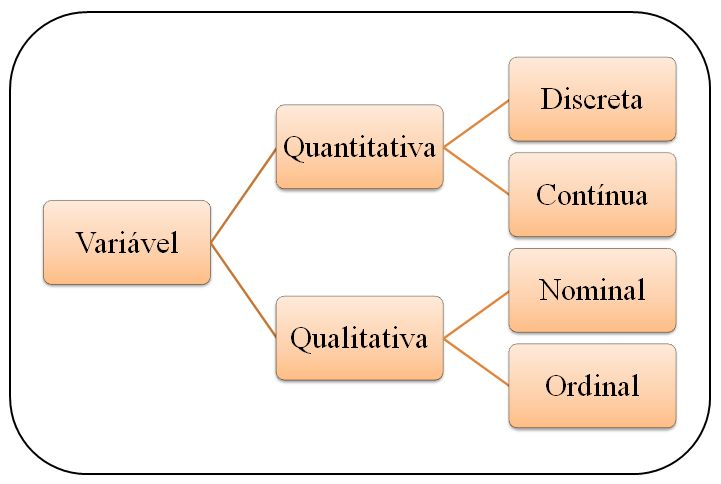
\includegraphics[width=10cm]{tipovariaveis.jpg}
	\caption{Classificação das variáveis}
	\label{fig:tipovariaveis}
\end{figure}


%------------------------------------------------

\section{Variáveis quantitativas}
São variáveis cujas possíveis realizações são números resultantes de uma contagem ou mensuração.\\

\begin{itemize}
	\item {\bf Variáveis Quantitativas Discretas:}
	São variáveis numéricas para as quais os possíveis valores formam um conjunto finito ou 
	enumerável de números, e que resultam, frequentemente, de uma contagem. Por exemplo, 
	a variável número de filhos, cujas possíveis realizações são 0, 1, 2, 3, $...$, é uma 
	variável quantitativa discreta.\\

	\item {\bf Variáveis Quantitativas Contínuas:}
	São variáveis numéricas para as quais os possíveis valores pertencem a um intervalo 
	de números reais e que resultam de uma mensuração. Por exemplo, a variável altura de 
	um indivíduo, cujas possíveis realizações são números reais positivos (por exemplo: 
	$1,60m$, $1,56m$, $1,75m$, $...$) é uma variável quantitativa contínua.\\
\end{itemize}

%------------------------------------------------

\section{Variáveis qualitativas}
São variáveis que apresentam como possíveis realizações uma qualidade (ou atributo) do indivíduo pesquisado.\\

\begin{itemize}
	\item {\bf Variáveis qualitativas nominais:} 
	São variáveis cujas possíveis realizações são atributos para os quais não existe nenhuma 
	ordenação. Por exemplo, a variável sexo, cujas possíveis realizações são masculino e 
	feminino, é uma variável qualitativa nominal pois suas realizações não tem nenhuma ordenação.\\

	\item {\bf Variáveis qualitativas ordinais:}
	São variáveis cujas possíveis realizações são atributos para os quais existe uma ordem. 
	Por exemplo, a variável grau de instrução, cujas possíveis realizações podem ser: ensino 
	fundamental, ensino médio e ensino superior; é uma variável qualitativa ordinal pois suas 
	possíveis realizações seguem uma ordem crescente que está atrelada aos anos de estudo concluídos.\\
\end{itemize}


\begin{example} \label{exemp:tipoVar}
	Classifique as variáveis apresentadas a seguir:

	%Foram utilizados "\,\,\," e "\," para o alinhamento ficar igual ao do \enumerate
	\begin{table}[h]
	\begin{tabular}{l l}
	\,\,\, a) \, Peso & \footnotesize\texttt{Resposta: quantitativa contínua}\\
	\,\,\, b) \, Classe social & \footnotesize\texttt{Resposta: qualitativa ordinal}\\
	\,\,\, c) \, Número de irmãos & \footnotesize\texttt{Resposta: quantitativa discreta}\\
	\,\,\, d) \, Tempo & \footnotesize\texttt{Resposta: quantitativa contínua}\\
	\,\,\, e) \, Cor dos olhos & \footnotesize\texttt{Resposta: qualitativa nominal}\\
	\,\,\, f) \ Raça de gatos & \footnotesize\texttt{Resposta: qualitativa nominal}\\
	\end{tabular}
	\end{table}
\end{example}
%\vspace{0.5cm}


%----------------------------------------------------------------------------------------
%	CHAPTER 5
%----------------------------------------------------------------------------------------

\chapterimage{chapter_head_3.pdf} % Chapter heading image

\chapter{Tabelas}
%------------------------------------------------

\section{Normas para construção de tabelas}

Os dados são apresentados em tabelas colocadas perto do ponto do texto em que são mencionadas pela primeira vez. As tabelas devem conter os seguintes elementos: título, cabeçalho, indicador de linha, célula e moldura, como mostrado no exemplo a seguir.\\

\begin{example} \label{exemp:elementosTabela}

	Considerando a Tabela \ref{tab:elementosdatabela}, apresentada a seguir, serão ilustrados os elementos que 
	compõem  uma tabela.

	\begin{table}[h]
	\caption{População do Brasil, segundo o sexo, de acordo com o Censo Demográfico 2010}
	\label{tab:elementosdatabela} 
	\vspace{0.1cm}
	\centering
	\begin{tabular}{l l}
	\toprule
	\textbf{Sexo} & \textbf{População residente}\\
	\midrule
	Homens & 93.406.990 \\
	Mulheres & 97.348.809 \\
	\hline
	Total & 190.755.799 \\
	\bottomrule
	\end{tabular} \\
	\vspace{0.1cm}\footnotesize Fonte: Censo Demográfico 2010. IBGE (2011).
	\end{table}

	
	\subsubsection{Elementos de uma tabela}
	
	\vspace{0.5cm}

	\begin{itemize}
	
	\item {\bf Título}: especifica o conteúdo da tabela.
	\begin{eBox} 
	Tabela \ref{tab:elementosdatabela}: População do Brasil, segundo o sexo, de acordo com o Censo 	
	Demográfico 2010  
	\end{eBox}
	
	O título deve ser colocado na parte superior da tabela.\\
	
	
	\item {\bf Cabeçalho}: especifica o conteúdo de cada coluna.
	\begin{eBox}
	\centering
	\begin{tabular}{l l}
	\toprule
	\textbf{Sexo} & \textbf{População residente}\\
	\midrule
	\end{tabular}
	\end{eBox}
	\hspace{0.5cm}	
	
	\item {\bf Indicador de linha}: é um conjunto de termos em que cada termo indica o conteúdo de uma linha.
	\begin{eBox}
	\centering
	\begin{tabular}{l l l}
	\midrule
	Homens & \hspace{2cm} & \\
	Mulheres & & \\
	\hline
	Total & & \\
	\bottomrule
	\end{tabular} \\
	\end{eBox}
	
	\hspace{0.5cm}		
	
	\item {\bf Célula}: resulta do cruzamento de uma linha com uma coluna e deve conter um dado numérico.
	\begin{eBox}
	\centering
	\begin{tabular}{l l l}
	\midrule
	& \hspace{2cm} & 93.406.990 \\
	& & 97.348.809 \\
	\hline
	& & 190.755.799 \\
	\bottomrule
	\end{tabular} \\
	\end{eBox}
	
	Nenhuma célula da tabela deve ficar em branco. Toda célula deve apresentar um número ou, se o dado não existir, deve-se colocar um traço $( - )$ na célula para indicar que aquele dado não existe.\\

	
	\item {\bf Moldura}: Entende-se por moldura o conjunto de traços que delimitam a tabela.
	\begin{eBox}
	\centering	
	\begin{tabular}{l l}
	\toprule
	\hspace{2cm} & \hspace{2cm} \\
	\midrule
	 &  \\
	 &  \\
	 \hline
	 &  \\
	\bottomrule
	\end{tabular} \\
	\end{eBox}
		
	A moldura é composta apenas por traços horizontais. Basicamente é composta por um traço superior e um inferior que delimitam a tabela e mais um traço abaixo do cabeçalho para delimitá-lo. Quando a última linha da tabela representa a soma das colunas (linha do Total) é costume fazer mais um traço horizontal acima desta linha para delimitá-la também. Pode-se, ainda, fazer traços verticais no interior da tabela para separar uma coluna da outra, porém, não se deve "fechar" as laterais da tabela com traços verticais.\\
	
	\item {\bf Fonte}: indica o responsável (pessoa física ou jurídica) pelos dados.
	\begin{eBox} 
	\footnotesize Fonte: Censo Demográfico 2010. IBGE (2011).  
	\end{eBox}
	
	A Fonte deve ser colocada na primeira linha do rodapé da tabela e precedida pela palavra {\itshape Fonte}. 
	Não é necessário indicar a fonte nos casos em que os dados forem obtidos pelo próprio pesquisador.

	\end{itemize}
\end{example}


%------------------------------------------------

\section{Tabelas de distribuição de frequências}
\vspace{0,3cm}
\subsection{Distribuição de frequências para dados qualitativos}
\vspace{0,3cm}

Quando observamos dados qualitativos, classificamos cada observação em determinada categoria. Depois, contamos o número de observações em cada categoria. A idéia é resumir as informações na forma de uma tabela que mostre essas contagens (frequências) por categoria.\\


\begin{example} \label{exemp:tabFreqQuali}

	Considere os dados brutos do grau de instrução de 36 indivíduos:
	
	\begin{center}
	\begin{tabular}{c c c c c c}
	\hline
	Fundamental & 	Médio & Médio & Superior & Médio & Médio \\
	Médio & Médio & Fundamental & Fundamental & Superior & Fundamental \\
	Superior & Fundamental & Médio & Médio & Médio & Médio \\
	Fundamental & Médio & Superior & Fundamental & Superior & Médio \\
	Médio & Fundamental & Médio & Médio & Médio & Fundamental \\
	Fundamental & Fundamental & Superior & Fundamental & Médio & Médio\\
	\hline	
	\end{tabular}
	\end{center}
	
	Contando os dados por categoria temos $12$ indivíduos cujo grau de instrução é o ensino fundamental, $18$ indivíduos com ensino médio e $6$ indivíduos com ensino superior. Assim, podemos resumir essas informações na Tabela \ref{tab:distfreqquali}.
	
	\begin{table}[h]
	\caption{Distribuição de frequências do grau de instrução de 36 indivíduos}
	\label{tab:distfreqquali} 
	\vspace{0.1cm}
	\centering
	\begin{tabular}{l c}
	\toprule
	\textbf{Grau de instrução} & \textbf{Frequências ($\bm{f_i}$)}\\
	\midrule
	Fundamental & 12 \\
	Médio & 18 \\
	Superior & 6 \\
	\hline
	Total & 36 \\
	\bottomrule
	\end{tabular} \\
	\end{table}
	

	As tabelas de distribuição de frequências podem conter, além das frequências (também conhecidas como frequências absolutas: $f_i$), as proporções (também conhecidas como frequências relativas: $fr_i$) e as porcentagens (também conhecidas como frequências percentuais: $fp_i$). As frequências relativas são calculadas dividindo-se cada frequência absoluta pelo total, enquanto as frequências percentuais são calculadas multiplicando-se cada frequência relativa por 100. Por exemplo, para o grau de instrução ensino fundamental, obtemos a frequência relativa fazendo $12/36=0,3333$, e a frequência percentual fazendo $0,3333 \times 100=33,33\%$, como pode-se observar na Tabela \ref{tab:distfreqquali2}.


	\begin{table}[h]
	\caption{Distribuição de frequências do grau de instrução de 36 indivíduos}
	\label{tab:distfreqquali2} 
	\vspace{0.1cm}
	\centering
	\begin{tabular}{l c c c}
	\toprule
	\textbf{Grau de instrução} & $\bm{f_i}$ & $\bm{fr_i}$ & $\bm{fp_i$}\\
	\midrule
	Fundamental & 12 & 0,3333 & 33,33\% \\
	Médio & 18 & 0,5000 & 50,00\% \\
	Superior & 6 & 0,1667 & 16,67\% \\
	\hline
	Total & 36 & 1,0000 & 100,00\% \\
	\bottomrule
	\end{tabular} \\
	\end{table}

\end{example}
\vspace{0.5cm}

Na Lista~\ref{lst:Rtab1} são apresentados os comandos do software R para organizar os dados do Exemplo~\ref{exemp:tabFreqQuali} em uma distribuição de frequências. 

\begin{scriptsize}
	\estiloR
	\begin{lstlisting}[caption={Comandos do software R}, label=lst:Rtab1]
	# Entrando com os dados no R:
	dados <- c("Fundamental","Médio","Médio","Superior","Médio","Médio",
			"Médio","Médio","Fundamental","Fundamental","Superior","Fundamental",
			"Superior","Fundamental","Médio","Médio","Médio","Médio",
			"Fundamental","Médio","Superior","Fundamental","Superior","Médio",
			"Médio","Fundamental","Médio","Médio","Médio","Fundamental",
			"Fundamental","Fundamental","Superior","Fundamental","Médio","Médio")
	
	# Mostrando os dados armazenados (OPCIONAL)
	dados
	
	# Gerando a distribuição de frequências
	tab <- table(dados)

	# Mostrando a distribuição de frequências
	tab
	
	# Gerando e mostrando as proporções
	tabprop <- prop.table(tab) ; tabprop
		
	\end{lstlisting}
\end{scriptsize}


\noindent {\bf Observação}: ao executar os comandos da Lista~\ref{lst:Rtab1}, os níveis da variável analisada aparecem na tabela de distribuição de frequências em ordem alfabética: \texttt{"Fundamental", "Médio", "Superior"}. Neste caso, a ordem alfabética também coincide com a ordem natural dos níveis dessa variável. Porém, se a ordem dos níveis de uma variável qualitativa ordinal não coincidir com a ordem alfabética, no R também é possível ordenar as categorias desta variável ao gerar uma tabela de distribuição de frequências. \\ 

Na Lista~\ref{lst:Rtab1.2} são apresentados os comandos para ordenar os níveis da variável (fator) "classe social" e assim gerar uma tabela de distribuição de frequências com os níveis desse fator devidamente ordenados. \\


\begin{scriptsize}
	\estiloR
	\begin{lstlisting}[caption={Comandos do software R}, label=lst:Rtab1.2]
	# Criando um vetor convertido em fator com níveis não ordenados
	cs <- factor(c("media", "baixa", "media", "alta", "baixa", "baixa", "alta", "media", "alta", "media"))

	# Gerando uma distribuição de frequências sem ordenar os níveis desse fator
	table(cs)	

	# Ordenando os níveis do fator cs (classe social)
	cs <- factor(cs, ord=T, levels=c("baixa", "media", "alta"))

	# Gerando uma distribuição de frequências com os níveis do fator ordenados
	table(cs)
	
	\end{lstlisting}
\end{scriptsize}

\noindent {\bf Observação}: ao executar os comandos da Lista~\ref{lst:Rtab1.2}, ns saída da linha $5$ os níveis do fator "grau" apresentados na tabela de distribuição de frequências aparecem na ordem: \texttt{"alto", "baixo","medio"}. Já na saída da linha $11$ eles aparecem na ordem: \texttt{"baixo", "medio", "alto"}, pois os níveis do fator foram previamente ordenados. \\




\subsection{Distribuição de frequências para dados quantitativos}
\vspace{0,3cm}

Dados quantitativos também podem ser agrupados em tabelas de distribuição de frequências, porém a construção da tabela é diferente para dados discretos e contínuos. \\


\subsubsection{Tabela para dados quantitativos discretos}
\vspace{0,3cm}

Para organizar uma tabela de distribuição de frequências para dados quantitativos discretos deve-se seguir os passos:

\begin{enumerate}
\item escreva os dados em ordem crescente (rol);
\item conte quantas vezes cada valor se repete (frequência);
\item organize a tabela apresentando os valores numéricos em ordem natural e suas respectivas frequências. \\
\end{enumerate}

\begin{example} \label{exemp:tabFreqQuanti}
	Considere os dados brutos do número de faltas ao trabalho de trinta funcionários:
	
	\begin{center}
	\begin{tabular}{c c c c c c c c c c c c c c c}
	\hline
	1 & 3 & 1 & 1 & 0 & 1 & 0 & 1 & 1 & 0 & 2 & 2 & 0 & 0 & 0 \\
	1 & 2 & 1 & 2 & 0 & 0 & 1 & 6 & 4 & 3 & 3 & 1 & 2 & 4 & 0 \\
	\hline
	\end{tabular}
	\end{center}
	
	Construa uma tabela de distribuição de frequências do número de faltas ao trabalho. \\
	
	\noindent \hspace{0.3cm}{\small\bf\sffamily Solução} \\
	
	Organizando os dados em ordem crescente temos:
	
	\begin{center}
	\begin{tabular}{c c c c c c c c c c c c c c c}
	\hline
	0 & 0 & 0 & 0 & 0 & 0 & 0 & 0 & 0 &  1 &  1 &  1 &  1 &  1 &  1 \\
	1 & 1 & 1 & 1 & 2 & 2 & 2 & 2 & 2 &  3 &  3 &  3 &  4 &  4 &  6 \\
	\hline
	\end{tabular}
	\end{center}
	
	Agora basta contar as frequências (quantidade de vezes que cada número ocorre) e montar a tabela de 
	distribuição de frequências (Tabela \ref{tab:distfreqquant1}). \\
	
	\noindent {\bf Observação}: Como o número de faltas $x_i=5$ não aparece no conjunto de dados brutos ele deve ser representado na tabela de distribuição de frequências como tendo frequência $f_i=0$.
	
	\begin{table}[h]
	\caption{Distribuição de frequências do número de faltas ao trabalho de trinta funcionários}
	\label{tab:distfreqquant1} 
	\vspace{0.1cm}
	\centering
	\begin{tabular}{c c c}
	\toprule
	\textbf{Número de faltas} & $\bm{f_i}$ & \\
	\midrule
	0 & 9 \\
	1 & 10 \\
	2 & 5 \\
	3 & 3 \\
	4 & 2 \\
	5 & 0 \\
	6 & 1 \\
	\hline
	Total & 30 \\
	\bottomrule
	\end{tabular} \\
	\end{table}
	
\end{example}

\vspace{0.5cm}

Na Lista~\ref{lst:Rtab2} são apresentados os comandos do software R para organizar os dados do Exemplo~\ref{exemp:tabFreqQuanti} em uma distribuição de frequências. \\

\begin{scriptsize}
	\estiloR
	\begin{lstlisting}[caption={Comandos do software R}, label=lst:Rtab2]
	# Entrando com os dados no R
	dados <- c(1,3,1,1,0,1,0,1,1,0,2,2,0,0,0,1,2,1,2,0,0,1,6,4,3,3,1,2,4,0)

	# Mostrando os dados armazenados
	dados

	# Tabela de distribuição de frequências
	tab <- table(dados)

	# Mostrando a tabela de distribuição de frequências
	tab

	\end{lstlisting}
\end{scriptsize}

\noindent {\bf Observação}: Ao executar os comandos do software R apresentados na Lista~\ref{lst:Rtab2} não irá aparecer na saída do software R o número de faltas $x_i=5$ com frequência $f_i=0$ como foi apresentado na Tabela~\ref{tab:distfreqquant1}. \\

Quando existirem muitos valores possíveis para a variável discreta (por exemplo, muitos valores entre 0 e 100) podemos construir uma tabela de distribuição de frequências do mesmo modo que faremos com uma variável contínua (agrupando os dados em classes). \\



\subsubsection{Tabela para dados quantitativos contínuos}
\vspace{0,3cm}

Ao contrário das variáveis discretas, as variáveis contínuas assumem, em geral, muitos valores. Isto quer dizer que se utilizássemos para variáveis contínuas tabelas de frequências iguais as tabelas das variáveis discretas teríamos uma tabela com muitas linhas, tornando-a pouco operacional. Para contornar este problema costuma-se descrever as variáveis quantitativas contínuas através de tabelas de frequências cujos valores $(x_i)$ da variável são agrupados em classes (intervalos).

A seguir é apresentado um exemplo de tabela de distribuição de frequências para variáveis contínuas. \\


\begin{example} \label{exemp:distfreqquant2} 

	Considere os dados brutos dos salários (em x sal. mín.) de 36 indivíduos:
	
	\begin{center} \label{dadosbrutossalarios}
	\begin{tabular}{c c c c c c c c c}
	\hline
	5,73  &  13,60  &  13,23  &  8,46  &  17,26  &  16,22  &  8,74  &  23,30  &  7,39 \\
	11,06  &  13,85  &  8,12  &  15,99  &  10,76  &  6,26  &  9,80  &  5,25  &  9,77 \\
	19,40  &  10,53  &  11,59  &  14,69  &  8,95  &  9,35  &  4,56  &  4,00  &  9,13 \\
	14,71  &  12,00  &  7,59  &  7,44  &  6,66  &  12,79  &  18,75  &  6,86  &  16,61 \\
	\hline
	\end{tabular}
	\end{center}
	
	Na Tabela~\ref{tab:distfreqquant2} é apresentada a distribuição de frequências dos salários dos 36 indivíduos 
	com os salários	agrupados em classes.
	
	
	\begin{table}[h]
	\caption{Distribuição de frequências dos salários de 36 indivíduos}
	\label{tab:distfreqquant2} 
	\vspace{0.1cm}
	\centering
	\begin{tabular}{l l l l}
	\toprule
	\textbf{Salários} & $\bm{f_i}$ & $\bm{fr_i}$ & $\bm{fp_i}$ \\
	\midrule
	\,\,\,$4,00 \vdash 8,00$  &  10  &  0,2778  &  27,78\% \\
	\,\,\,$8,00 \vdash 12,00$  &  12  &  0,3333  &  33,33\% \\
	$12,00 \vdash 16,00$  &  8  &  0,2222  &  22,22\% \\
	$16,00 \vdash 20,00$  &  5  &  0,1389  &  13,89\% \\
	$20,00 \vdash 24,00$  &  1  &  0,0278  &  2,78\% \\	
	\hline
	Total  &  36  &  1,0000  &  100,00\% \\
	\bottomrule
	\end{tabular} \\
	\end{table}
	
	Observe que procedendo-se desse modo, ao resumir os dados referentes a uma variável contínua, 
	perde-se alguma informação. Por exemplo, na classe que vai de 12 a 16, não sabemos quais são os valores 
	exatos dos oito salários, a não ser que investiguemos o conjunto de dados original.
	
\end{example}
\vspace{0.5cm}

Note que estamos usando a notação $a \vdash b$ para o intervalo de números contendo o extremo $a$ mas não contendo o extremo $b$. Podemos também usar a notação  $[a, b)$  para designar o mesmo intervalo. 

Os comandos do software R para a obtenção da distribuição de frequências do Exemplo~\ref{exemp:distfreqquant2} são apresentados na Lista~\ref{lst:Rtab3}.


\begin{scriptsize}
	\estiloR
	\begin{lstlisting}[caption={Comandos do software R}, label=lst:Rtab3]
	# Entrando com os dados no R
	dados <- c(5.73, 13.60, 13.23, 8.46, 17.26, 16.22, 8.74, 23.30, 7.39,
			11.06, 13.85, 8.12, 15.99, 10.76, 6.26, 9.80, 5.25, 9.77,
			19.40, 10.53, 11.59, 14.69, 8.95, 9.35, 4.56, 4.00, 9.13,
			14.71, 12.00, 7.59, 7.44, 6.66, 12.79, 18.75, 6.86, 16.61)
	
	# Mostrando os dados armazenados (OPCIONAL)
	dados
	
	# Organizando os dados em ordem crescente (OPCIONAL)
	sort(dados)
	
	# Distribuição de frequências
	hist(dados, plot=F, breaks=c(4,8,12,16,20,24), right=F)
	
	\end{lstlisting}
\end{scriptsize}

\noindent {\bf Observações referentes à Lista~\ref{lst:Rtab3}}: 

\begin{enumerate}[label=\alph*)]

\item no comando \texttt{hist()} os limites das classes foram especificados usando o argumento \texttt{ breaks=c(4,8,12,16,20,24)};

\item o padrão do comando \texttt{hist()} é gerar intervalos fechados à direita. Para que sejam gerados intervalos abertos à direita deve-se utilizar o argumento \texttt{right=F};

\item por padrão, o comando \texttt{hist()} gera um gráfico (histograma). Como dentro do comando \texttt{hist()} foi usado o argumento \texttt{plot=F}, ao invés de gerar um gráfico é mostrada uma saída em forma de lista contendo os limites das classe em \texttt{\$breaks}, as frequências das classes em \texttt{\$counts}, os pontos médios das classes em \texttt{\$mids}, etc; \\

\end{enumerate}
 

A escolha dos intervalos pode ser feita arbitrariamente e a familiaridade do pesquisador com os dados é que lhe indicará quantas e quais classes devem ser usadas. Quando determinados intervalos de classes tiverem algum significado prático para o pesquisador, ele poderá simplesmente escolher estes intervalos. 

Não existe um número "ideal" de classes para um conjunto de dados, embora existam fórmulas para estabelecer quantas classes devem ser construídas. Vejamos, a seguir um critério para a construção das classes. \\


\subsubsection*{Passos para construção de uma tabela de distribuição de frequências para dados contínuos}

\begin{enumerate}
	\item Organize os dados em ordem crescente (rol); \\
	
	\item{Determine o número de classes (k):	
	\begin{enumerate}
		\item Se $n \leq 100$ utilize $k=\sqrt{n}$;
		\item Se $n>100$ utilize $k = 1+3,22 \log{n}$;
	\end{enumerate}
	{\bf Observação}: Arredonde o valor de $k$ para o valor inteiro mais próximo. \\
		}
		
	\item Encontre o menor ($X_{min}$) e o maior ($X_{max}$) valor do conjunto de dados; \\
	
	\item Calcule a amplitude ($A$), que é a diferença entre o maior e o menor valor:
	\begin{center}
	$A = X_{max}-X_{min}$
	\end{center}
	
	\item Divida a amplitude total pelo número de classes para obter a amplitude das classes ($c$):
	\begin{center}
	$c=A/k$
	\end{center}
	{\bf Observação}: Pode ser conveniente arredondar o valor de $c$ para o valor um pouco maior. 
	Por exemplo, se ocorrer $c=4,21$ arredonde para $c=4,25$ ou para $c=4,3$. \\
	
	\item Organize as classes, iniciando a primeira classe em $LI_1$ (limite inferior da 1ª classe), em que $LI_1$ pode ser o menor dado ($X_{min}$) ou pode ser um valor menor do que ele. Depois basta somar a amplitude das classes ($c$) a este valor para obter $LS_1$ (limite superior da 1ª classe), ou seja, $LS_1=LI_1+c$. O limite inferior da 2ª classe ($LI_2$) será igual ao limite superior da 1ª classe, ou seja, $LI_2=LS_1$. Para obter $LS_2$ (limite superior da segunda classe) basta somar a amplitude das classes ($c$) ao limite inferior da mesma classe, ou seja, $LS_2=LI_2+c$. Para obter os demais intervalos de classes repita o processo sucessivamente até completar o número de classes ($k$). \\
	
	\item Depois de construir todas as ($k$) classes, conte quantos dados têm dentro de cada classe e anote os resultados na coluna das frequências ($f_i$). \\
	
	{\bf Observações}: (a) A primeira e a última classe não podem ter frequência nula, já nas demais classes pode ocorrer frequência nula. (b) Se ocorrer um dado igual ao limite superior de uma classe este valor deve ser computado na frequência da classe seguinte pois estão sendo considerados intervalos de classes abertos à direita, ou seja, intervalos do tipo $[a,b)$. \\
	
\end{enumerate}



\begin{example} \label{exemp:distfreqquant3}

Construiremos uma tabela de distribuição de frequências considerando os dados de salários (x sal. mín.) de 36 indivíduos apresentados no Exemplo~\ref{exemp:distfreqquant2}. Para isso, serão seguidos os passos apresentados. \\

\begin{enumerate}
\item Dados em ordem crescente (rol):

	\begin{center}
	\begin{tabular}{c c c c c c c c c}
	\hline
	4,00  &  4,56  &  5,25  &  5,73  &  6,26  &  6,66	&	6,86  &  7,39  &  7,44 \\
	7,59  &  8,12  &  8,46	&	8,74  &  8,95  &  9,13  &  9,35  &  9,77  &  9,80 \\
	10,53  &  10,76  &  11,06  &	11,59  &  12,00  &  12,79	&	13,23	&  13,60  &  13,85  \\
	14,69  &  14,71  &  15,99	&	16,22  &  16,61  &  17,26	&  18,75	&  19,40  &  23,30 \\
	\hline
	\end{tabular}
	\end{center}
	
	\item Número de classes: $k=\sqrt{n}=\sqrt{36}=6$; \\
	
	\item Mínimo e máximo: $X_{min}=4,00$ e $X_{max}=23,30$; \\
	
	\item Amplitude total: $A=X_{max}-X_{min}=23,30-4,00=19,30$; \\
	
	\item Amplitude das classes: $c= A/k=19,30/6=3,22$, que arredondaremos para  $c=3,5$; \\
	
	\item Classes: iniciaremos o limite inferior da 1ª classe ($LI_1$) em $4,00$ (também poderíamos ter iniciado em um valor menor do que $4,00$) e depois iremos somando $c=3,5$ para obter os	limites das demais classes:
	

	\begin{center}
	\begin{tabular}{l l l}
	$LI_1=4,0$       & , & $LS_1=4,0+c=4,0+3,5=7,5$ \\	
	$LI_2=LS_1=7,5$  & , & $LS_2=7,5+c=7,5+3,5=11,0$ \\	
	$LI_3=LS_2=11,0$ & , & $LS_3=11,0+c=11,0+3,5=14,5$ \\	
	$LI_4=LS_3=14,5$ & , & $LS_4=14,5+c=14,5+3,5=18,0$ \\	
	$LI_5=LS_4=18,0$ & , & $LS_5=18,0+c=18,0+3,5=21,5$ \\	
	$LI_6=LS_5=21,5$ & , & $LS_6=21,5+c=21,5+3,5=25,0$ \\	
	\end{tabular}
	\end{center}
	
	Na Tabela~\ref{tab:distfreqquant3} são apresentadas as classes de salários obtidas. Para finaizar a tabela basta observar o conjunto de dados ordenados e contar quantos dados tem em cada classe.
	
	\begin{table}[h]
	\caption{Classes de salários}
	\label{tab:distfreqquant3} 
	\vspace{0.1cm}
	\centering
	\begin{tabular}{l c l}
	\toprule
	\textbf{Salários} & $\bm{f_i}$ & \\
	\midrule
	\,\,\,$4,0 \vdash 7,5$  &  ? & \\
	\,\,\,$7,5 \vdash 11,0$  &  ? & \\
	$11,0 \vdash 14,5$  &  ?  & \\
	$14,5 \vdash 18,0$  & ? & \\
	$18,0 \vdash 21,5$  &  ? & \\	
	$21,5 \vdash 25,0$  &  ? & \\	
	\hline
	Total  &  ? & \\
	\bottomrule
	\end{tabular} \\
	\end{table}
	
	\vspace{0.4 cm}
	
	\item Frequências: para facilitar a contagem das frequências, neste exemplo, destacamos os dados dentro de cada classe de salários com cores diferentes. {\bf Observação}: não é necessário fazer este procedimento de separar os dados por cores diferentes, foi feito aqui apenas como recurso didático.\\
	
	
	\begin{center}
	\begin{tabular}{c c c c c c c c c}
	\hline
	\textcolor{ocre}{\bf 4,00}  &  \textcolor{ocre}{\bf 4,56}  &  \textcolor{ocre}{\bf 5,25}  &  
	\textcolor{ocre}{\bf 5,73}  &  \textcolor{ocre}{\bf 6,26}  &  \textcolor{ocre}{\bf 6,66}	&	
	\textcolor{ocre}{\bf 6,86}  &  \textcolor{ocre}{\bf 7,39}  &  \textcolor{ocre}{\bf 7,44} \\
	
	{\bf 7,59}  &  {\bf 8,12}  &  {\bf 8,46}	&	{\bf 8,74}  &  {\bf 8,95}  &  {\bf 9,13}  &  
	{\bf 9,35}  &  {\bf 9,77}  &  {\bf 9,80} \\
	{\bf 10,53}  &  {\bf 10,76}  &  
	
	\textcolor{verdescuro}{\bf 11,06}  &	\textcolor{verdescuro}{\bf 11,59}  &  \textcolor{verdescuro}{\bf 12,00}  &  
	\textcolor{verdescuro}{\bf 12,79}	&	\textcolor{verdescuro}{\bf 13,23}	&  \textcolor{verdescuro}{\bf 13,60}  &  
	\textcolor{verdescuro}{\bf 13,85}  \\
	
	
	\textcolor{ocre}{\bf 14,69}  &  \textcolor{ocre}{\bf 14,71}  &  \textcolor{ocre}{\bf 15,99}	&	
	\textcolor{ocre}{\bf 16,22}  &  \textcolor{ocre}{\bf 16,61}  &  \textcolor{ocre}{\bf 17,26}	&  
	
	{\bf 18,75}	&  {\bf 19,40}  &  
	
	\textcolor{ocre}{\bf 23,30} \\
	\hline
	\end{tabular}
	\end{center}
	
	\vspace{0.4 cm}
	
	 Na Tabela~\ref{tab:distfreqquant4} pode-se observar a distribuição de frequências dos salários 
	 de 36 indivíduos. \\
	
	\begin{table}[h]
	\caption{Distribuição de frequências dos salários de 36 indivíduos}
	\label{tab:distfreqquant4} 
	\vspace{0.1cm}
	\centering
	\begin{tabular}{l c l}
	\toprule
	\textbf{Salários} & $\bm{f_i}$ & \\
	\midrule
	\,\,\,$4,0 \vdash 7,5$  &  9 & \\
	\,\,\,$7,5 \vdash 11,0$  & 11 & \\
	$11,0 \vdash 14,5$  &  7  & \\
	$14,5 \vdash 18,0$  & 6 & \\
	$18,0 \vdash 21,5$  &  2 & \\	
	$21,5 \vdash 25,0$  &  1 & \\	
	\hline
	Total  &  36 & \\
	\bottomrule
	\end{tabular} \\
	\end{table}

\end{enumerate}

\end{example}

\vspace{0,5 cm}

Observe, neste exemplo, que se ao invés de arredondar a amplitude da classe $c$ para $3,5$ tivéssemos arredondado para $4,0$ então a sexta classe (última) seria $24 \vdash 28$ e não teria nenhum elemento; ou seja, na realidade não teríamos seis classes mas apenas cinco (pois a última classe teria frequência igual a zero). Utilizando esta forma de montar as classes precisamos tomar cuidado ao arredondar a amplitude da classe e ao escolher o limite inferior da primeira classe. 

Os comandos do software R para a obtenção da distribuição de frequências do Exemplo~\ref{exemp:distfreqquant3} são apresentados na Lista~\ref{lst:Rtab4}. \\


\begin{scriptsize}
	\estiloR
	\begin{lstlisting}[caption={Comandos do software R}, label=lst:Rtab4]
	# Entrando com os dados no R
	dados <- c(5.73, 13.60, 13.23, 8.46, 17.26, 16.22, 8.74, 23.30, 7.39,
			11.06, 13.85, 8.12, 15.99, 10.76, 6.26, 9.80, 5.25, 9.77,
			19.40, 10.53, 11.59, 14.69, 8.95, 9.35, 4.56, 4.00, 9.13,
			14.71, 12.00, 7.59, 7.44, 6.66, 12.79, 18.75, 6.86, 16.61)
	
	# Distribuição de frequências
	hist(dados, plot=F, breaks=c(4,7.5,11,14.5,18,21.5,25), right=F)
	
	\end{lstlisting}
\end{scriptsize}


Pode-se, ainda, agrupar os dados em uma distribuição de frequências deixando que o software R utilize um critério próprio para escolha do número de classes e das próprias classes, sendo que para isso basta não utilizar o argumento \texttt{breaks=c(...)} dentro do comando \texttt{hist()}. Na Lista~\ref{lst:Rtab5} são apresentados os comandos do R para obtenção de uma distribuição de frequências usando o critério do R para obtenção das classes. \\


\begin{scriptsize}
	\estiloR
	\begin{lstlisting}[caption={Comandos do software R}, label=lst:Rtab5]
	# Entrando com os dados no R
	dados <- c(5.73, 13.60, 13.23, 8.46, 17.26, 16.22, 8.74, 23.30, 7.39,
			11.06, 13.85, 8.12, 15.99, 10.76, 6.26, 9.80, 5.25, 9.77,
			19.40, 10.53, 11.59, 14.69, 8.95, 9.35, 4.56, 4.00, 9.13,
			14.71, 12.00, 7.59, 7.44, 6.66, 12.79, 18.75, 6.86, 16.61)
	
	# Distribuição de frequências
	hist(dados, plot=F, right=F)
	
	\end{lstlisting}
\end{scriptsize}


%----------------------------------------------------------------------------------------
%	CHAPTER 6
%----------------------------------------------------------------------------------------

\chapterimage{chapter_head_3.pdf} % Chapter heading image

\chapter{Gráficos}
%------------------------------------------------

\section{Gráficos de colunas e barras}

\subsection{Gráfico de colunas (ou gráfico de barras verticais)}

O gráfico de colunas é um tipo de gráfico de barras, porém, nesse caso as barras são verticais (colunas). 

\subsubsection{Passos para construir um gráfico de colunas} 

\begin{enumerate}
\item desenhe o sistema de eixos cartesianos;

\item anote as categorias da variável estudada no eixo das abscissas (eixo horizontal);

\item escreva as frequências ou as frequências relativas (proporções) ou as frequências percentuais (porcentagens) no eixo das ordenadas (eixo vertical), obedecendo uma escala;

\item desenhe barras verticais (colunas) de mesma largura, separadas por um espaço, para representar as categorias da variável em estudo. A altura de cada barra deve ser dada pela frequência da categoria;

\item coloque legenda nos dois eixos (nomes dos eixos) e título na figura. \\

\end{enumerate}


\begin{example} \label{exemp:grafcol} 

No Exemplo~\ref{exemp:tabFreqQuali} foi construída uma tabela de distribuição de frequências para a variável grau de instrução (Tabela~\ref{tab:distfreqquali}). Esta tabela é apresentada novamente para facilitar a construção do gráfico de colunas.


\begin{table}[h]
	\begin{rBox}
	\captionsetup{labelformat=empty}
	\caption{\color{olivine!130}{Recordando a Tabela~\ref{tab:distfreqquali}}}
	\centering
	{\color{olivine!130} \begin{tabular}{l c}
	\toprule
	\textbf{Grau de instrução} & $\bm{f_i}$\\
	\midrule
	Fundamental & 12 \\
	Médio & 18 \\
	Superior & 6 \\
	\hline
	Total & 36 \\
	\bottomrule
	\end{tabular}} \\
	\end{rBox}
\end{table}


Podemos representar graficamente esta tabela de distribuição de frequências por meio de um gráfico de colunas (Figura~\ref{fig:grafcol}).

\begin{figure}[h!]
\centering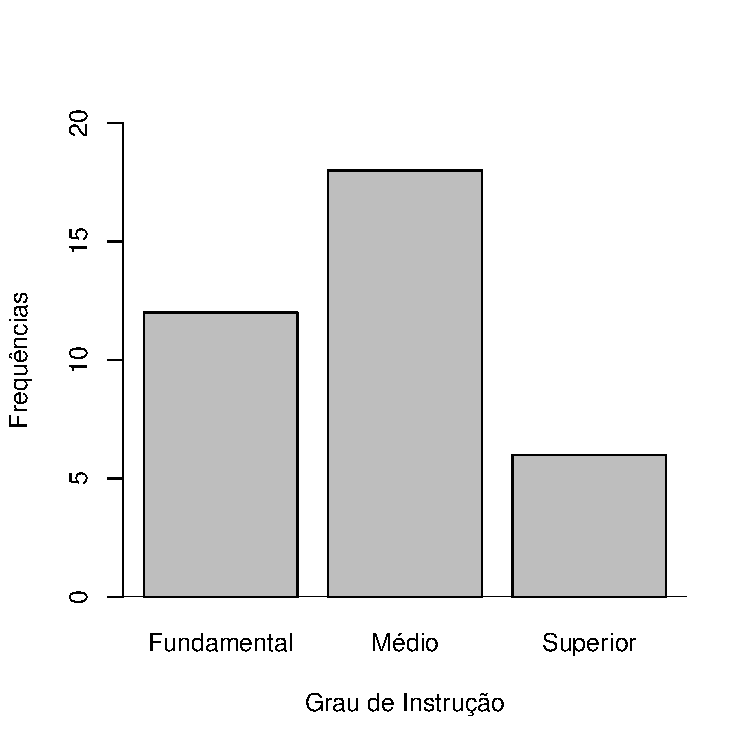
\includegraphics[trim=0 0 0 1.5cm, scale=0.8]{grafcol.pdf}
\setlength{\abovecaptionskip}{0.5pt}
\caption{Gráfico de colunas do grau de instrução}
\label{fig:grafcol} % Unique label used for referencing the figure in-text
\end{figure}

\end{example}

%\vspace{0,3 cm}

Na Lista~\ref{lst:Rgraf2} são apresentados os comandos do software R para fazer o gráfico de colunas (ou barras verticais).  \\

\begin{scriptsize}
	\estiloR
	\begin{lstlisting}[caption={Comandos do software R}, label=lst:Rgraf2]
	# Entrando com os dados no R:
	dados <- c("Fundamental","Médio","Médio","Superior","Médio","Médio",
			"Médio","Médio","Fundamental","Fundamental","Superior","Fundamental",
			"Superior","Fundamental","Médio","Médio","Médio","Médio",
			"Fundamental","Médio","Superior","Fundamental","Superior","Médio",
			"Médio","Fundamental","Médio","Médio","Médio","Fundamental",
			"Fundamental","Fundamental","Superior","Fundamental","Médio","Médio")
	
	# Mostrando os dados armazenados (OPCIONAL)
	dados
	
	# Gerando a distribuição de frequências
	tab <- table(dados)

	# Mostrando a distribuição de frequências (OPCIONAL)
	tab
	
	# Gerando o gráfico de colunas
	barplot(tab, ylim=c(0,20), xlab="Grau de Instrução", ylab="Frequências")
	abline(h=0)
	
	# Gerando o gráfico de colunas com título
	barplot(tab, ylim=c(0,20), xlab="Grau de Instrução", ylab="Frequências",
			main="Gráfico de colunas do grau de instrução")
	abline(h=0)
	
	\end{lstlisting}
\end{scriptsize}

\vspace{2 cm}

\noindent {\bf Observações referentes à Lista~\ref{lst:Rgraf2}}: 

\begin{enumerate}[label=\alph*)]

\item o argumento \texttt{ylim} especifica os limites do eixo {\itshape y} (eixo das ordenadas). Assim, \texttt{ylim=c(0,20)} especifica que o eixo {\itshape y} inicia em $y=0$ e termina em $y=20$;

\item os argumentos \texttt{xlab} e \texttt{ylab} especificam os nomes dos eixos {\itshape x} e {\itshape y}, respectivamente;

\item o comando \texttt{abline(h=0)} faz uma linha horizontal passando por $y=0$.

\end{enumerate}


\subsection{Gráfico de barras (ou gráfico de barras horizontais)}

O gráfico de barras (ou gráfico de barras horizontais) é usado para apresentar variáveis qualitativas, sejam elas nominais ou ordinais. Um gráfico de barras é a representação gráfica de uma distribuição de frequências de dados qualitativos. \\ 


\subsubsection{Passos para construir um gráfico de barras} 

\begin{enumerate}
	\item desenhe o sistema de eixos cartesianos;
	
	\item anote as categorias da variável estudada no eixo das ordenadas (eixo vertical);

	\item escreva as frequências ou as frequências relativas (proporções) ou as frequências percentuais (porcentagens) no eixo das abscissas (eixo horizontal), obedecendo uma escala;
	
	\item desenhe barras horizontais de mesma largura, separadas por um espaço, para representar 
	as categorias da variável em estudo. O comprimento de cada barra deve ser dado pela frequência da categoria;

	\item coloque legenda nos dois eixos (nomes dos eixos) e título na figura. \\
\end{enumerate}



\begin{example} \label{exemp:grafbar} 

No Exemplo~\ref{exemp:tabFreqQuali} foi construída uma tabela de distribuição de frequências para a variável grau de instrução (Tabela~\ref{tab:distfreqquali}). Podemos representar graficamente esta tabela de distribuição de frequências por meio de um gráfico de barras (Figura~\ref{fig:grafbar}).

\begin{figure}[h!]
\centering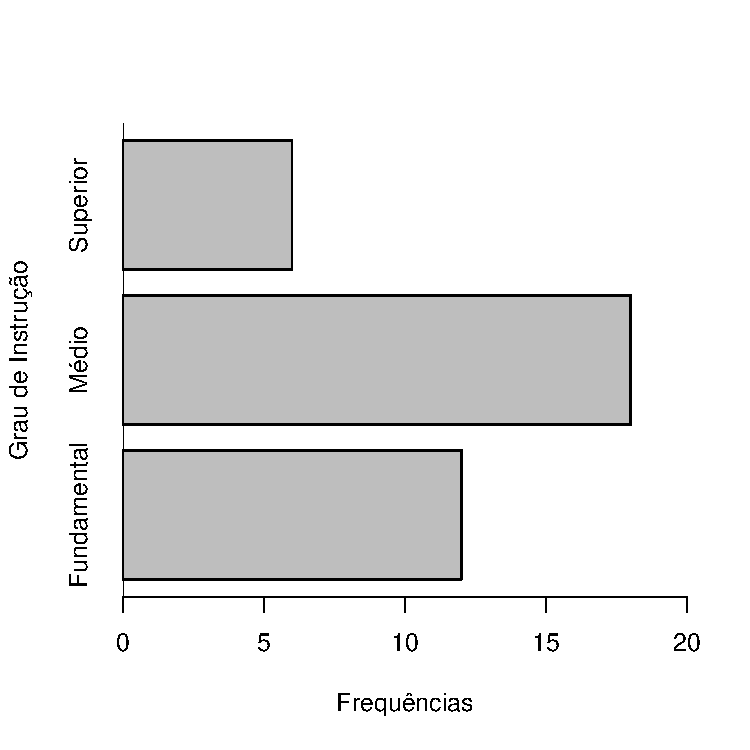
\includegraphics[trim=0 0 0 1.5cm, scale=0.8]{grafbar.pdf}
\setlength{\abovecaptionskip}{0.5pt}
\caption{Gráfico de barras do grau de instrução}
\label{fig:grafbar} % Unique label used for referencing the figure in-text
\end{figure}


\end{example}

%\vspace{0,3 cm}

Na Lista~\ref{lst:Rgraf1} são apresentados os comandos do software R para fazer o gráfico de barras horizontais. \\ 


\begin{scriptsize}
	\estiloR
	\begin{lstlisting}[caption={Comandos do software R}, label=lst:Rgraf1]
	# Entrando com os dados no R:
	dados <- c("Fundamental","Médio","Médio","Superior","Médio","Médio",
			"Médio","Médio","Fundamental","Fundamental","Superior","Fundamental",
			"Superior","Fundamental","Médio","Médio","Médio","Médio",
			"Fundamental","Médio","Superior","Fundamental","Superior","Médio",
			"Médio","Fundamental","Médio","Médio","Médio","Fundamental",
			"Fundamental","Fundamental","Superior","Fundamental","Médio","Médio")
	
	# Mostrando os dados armazenados (OPCIONAL)
	dados
	
	# Gerando a distribuição de frequências
	tab <- table(dados)

	# Mostrando a distribuição de frequências (OPCIONAL)
	tab
	
	# Gerando o gráfico de barras horizontais
	barplot(tab, horiz=T, xlim=c(0,20), xlab="Frequências", 
			ylab="Grau de Instrução")
	abline(v=0)
	
	\end{lstlisting}
\end{scriptsize}


\vspace{0,5 cm}

\noindent {\bf Observações referentes à Lista~\ref{lst:Rgraf1}}: 

\begin{enumerate}[label=\alph*)]

\item o argumento \texttt{horiz=T} faz com que as barras sejam geradas na posição horizontal;

\item o argumento \texttt{xlim} especifica os limites do eixo {\itshape x} (eixo das abscissas). Assim, \texttt{xlim=c(0,20)} especifica que o eixo {\itshape x} inicia em $x=0$ e termina em $x=20$;

\item o argumento \texttt{abline(v=0)} faz uma linha vertical passando por $x=0$.

\end{enumerate}



%------------------------------------------------

\section{Gráfico de setores}

O gráfico de setores (ou gráfico de pizza) é especialmente indicado para apresentar variáveis qualitativas, desde que o número de categorias seja pequeno.


\subsubsection{Passos para construir um gráfico de setores} 


\begin{enumerate}
\item desenhe uma circunferência (com 360°). Essa circunferência representará o total, ou seja, 100\% dos dados;

\item divida a circunferência em tantos setores quantas sejam as categorias da variável em estudo, mas é preciso calcular o ângulo de cada setor. O ângulo é igual a proporção da categoria multiplicada por 360°;

\item marque na circunferência os ângulos calculados e desenhe os raios passando pelos ângulos;

\item pinte cada categoria de uma cor, escreva as legendas das categorias e coloque título na figura. \\

\end{enumerate}



\begin{example} \label{exemp:grafset} 

No Exemplo~\ref{exemp:tabFreqQuali} foi construída uma tabela de distribuição de frequências para a variável grau de instrução (Tabela~\ref{tab:distfreqquali}). Podemos representar graficamente esta tabela de distribuição de frequências por meio de um gráfico de setores(Figura~\ref{fig:grafset2d}).

Para construir o gráfico de setores calculamos as proporções de cada categoria e depois multiplicamos por 360° para encontrar o ângulo de cada setor:

\begin{table}[h]
	\begin{eBox}
	\centering
	{\color{ocre} \begin{tabular}{l l l}
	\toprule
	Fundamental & $12/36=0,3333$ & $0,3333 \times 360^{\circ} \approx 120^{\circ}$ \\
	Médio & $18/36=0,5000$ & $0,5000 \times 360^{\circ} = 180^{\circ}$ \\
	Superior & $6/36=0,1667$ & $0,1667 \times 360^{\circ} \approx 60^{\circ}$ \\
	\bottomrule
	\end{tabular}} \\
	\end{eBox}
\end{table}

\vspace{2cm}

\begin{figure}[h!]
\centering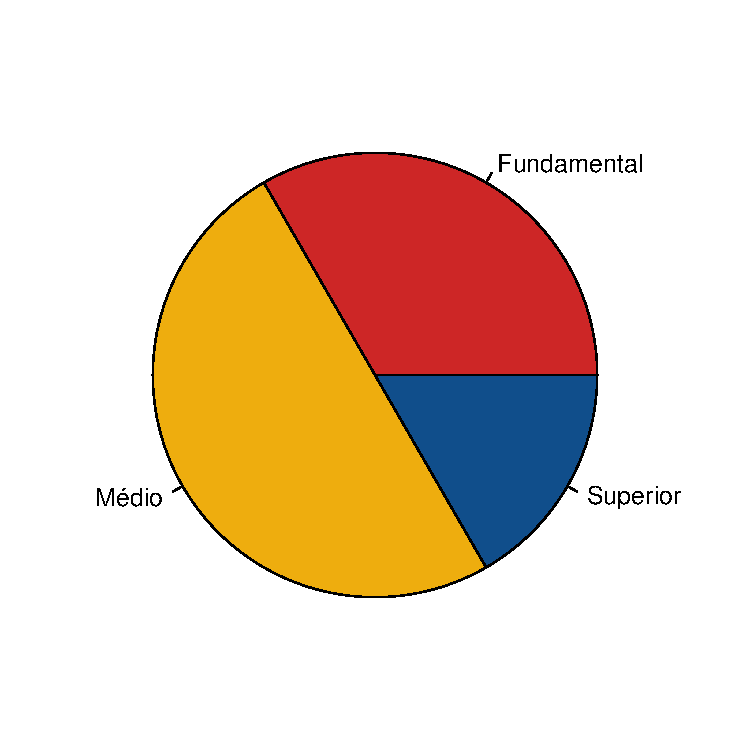
\includegraphics[trim=0 2cm 0 2cm, scale=0.8]{grafset2d.pdf}
\setlength{\abovecaptionskip}{0.5pt}
\caption{Gráfico de setores do grau de instrução}
\label{fig:grafset2d} % Unique label used for referencing the figure in-text
\end{figure}

Observe que o setor do ensino fundamental tem um ângulo de 120º, o setor do ensino médio tem um ângulo de 180º e o setor do ensino superior tem um ângulo de 60º. \\


Outra forma de apresentação mais elegante do gráfico de setores é utilizando um gráfico 3D. Na Figura~\ref{fig:grafset3d} é apresentado um gráfico de setores 3D feito com o pacote \texttt{plotrix} do software R.


\begin{figure}[h!]
\centering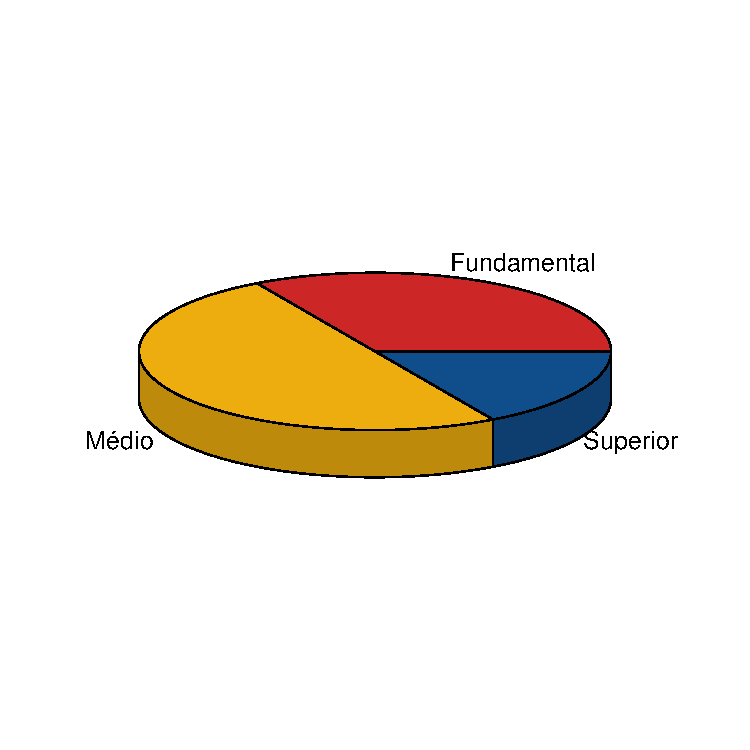
\includegraphics[trim=0 4cm 0 3cm, scale=0.8]{grafset3d.pdf}
\setlength{\abovecaptionskip}{0.5pt}
\caption{Gráfico de setores 3D do grau de instrução}
\label{fig:grafset3d} % Unique label used for referencing the figure in-text
\end{figure}

%\vspace{4 cm}

\end{example}

\vspace{0,5 cm}

Na Lista~\ref{lst:Rgraf3} são apresentados os comandos do software R para fazer os gráficos de setores 2D (Figura~\ref{fig:grafset2d}) e 3D (Figura~\ref{fig:grafset3d}).  \\

%\vspace{1 cm}

\begin{scriptsize}
	\estiloR
	\begin{lstlisting}[caption={Comandos do software R}, label=lst:Rgraf3]
	# Entrando com os dados no R:
	dados <- c("Fundamental","Médio","Médio","Superior","Médio","Médio",
			"Médio","Médio","Fundamental","Fundamental","Superior","Fundamental",
			"Superior","Fundamental","Médio","Médio","Médio","Médio",
			"Fundamental","Médio","Superior","Fundamental","Superior","Médio",
			"Médio","Fundamental","Médio","Médio","Médio","Fundamental",
			"Fundamental","Fundamental","Superior","Fundamental","Médio","Médio")
	
	# Mostrando os dados armazenados (OPCIONAL)
	dados
	
	# Gerando a distribuição de frequências
	tab <- table(dados)

	# Mostrando a distribuição de frequências (OPCIONAL)
	tab
	
	# Gráfico de setores 2D
	pie(tab,col=c("firebrick3","darkgoldenrod2","dodgerblue4"))


	#Gráfico de setores 3D
	
	# Carregando o pacote plotrix (precisa estar instalado)
	library(plotrix) 
	
	# Plotando o gráfico:
	pie3D(tab, col=c("firebrick3","darkgoldenrod2","dodgerblue4"), 
			labels=names(tab), labelcex=1)
	
	\end{lstlisting}
\end{scriptsize}

\vspace{0.3 cm}

Observe, na Lista~\ref{lst:Rgraf3}, que dentro dos comandos usados para gerar os gráficos de setores (\texttt{pie()} e \texttt{pie3D()}) foi utilizado o argumento \texttt{col}, que serve para especificar as cores do gráfico. Neste exemplo foram usadas as cores {\itshape "firebrick3"}, {\itshape "darkgoldenrod2"} e {\itshape "dodgerblue4"}. Se digitar o comando \texttt{colors()} no R irá aparecer uma lista com os nomes de mais de 600 cores (porém sem mostrar as cores). Para observar diferentes cores e seus respectivos nomes para usá-las no software R pode-se consultar uma paleta de cores. Em uma consulta rápida na internet podem ser encontradas várias paletas de cores para o software R. Uma paleta de cores interessante pode ser acessada em: \url{http://www.stat.columbia.edu/~tzheng/files/Rcolor.pdf}. Outra forma de visualizar exemplos de cores no R é digitando o comando \texttt{demo(colors)} diretamente no console do R. 

Além da possibilidade de alterar as cores também é possível fazer alterações em outros parâmetros gráficos. Para visualizar os parâmetros gráficos que podem ser alterados basta digitar no console \texttt{?pie} ou \texttt{?pie3D}, ou seja, o nome do comando antecedido pelo sinal de interrogação.



%------------------------------------------------

\section{Diagrama de linhas}


O diagrama de linhas é utilizado para apresentar graficamente dados quantitativos discretos organizados em uma tabela de distribuição de frequências. 

\subsubsection{Passos para construir um diagrama de linhas}

\begin{enumerate}
	\item desenhe o sistema de eixos cartesianos;
	
	\item no eixo das abscissas (eixo horizontal) apresente uma escala (de um em um, ou de dois em dois, ...) de valores para a variável;
	
	\item no eixo das ordenadas (eixo vertical) apresente uma escala de valores para as frequências;
	
	\item desenhe linhas verticais a partir dos valores assumidos pela variável no eixo das abscissas. Os comprimentos das barras são dados pelas frequências ou pelas porcentagens;
	
	\item coloque legendas nos dois eixos e título na figura. \\ \\
\end{enumerate}


\begin{example}

No Exemplo~\ref{exemp:tabFreqQuanti} foi construída uma tabela de distribuição de frequências para a variável  número de faltas ao trabalho (Tabela~\ref{tab:distfreqquant1}). Esta tabela é apresentada novamente para facilitar a construção do diagrama de linhas.


\begin{table}[h]
	\begin{rBox}
	\captionsetup{labelformat=empty}
	\caption{\color{olivine!130}{Recordando a Tabela~\ref{tab:distfreqquant1}}}
	\centering
	{\color{olivine!130}\begin{tabular}{c c c}
	\toprule
	\textbf{Número de faltas} & $\bm{f_i}$ & \\
	\midrule
	0 & 9 \\
	1 & 10 \\
	2 & 5 \\
	3 & 3 \\
	4 & 2 \\
	5 & 0 \\
	6 & 1 \\
	\hline
	Total & 30 \\
	\bottomrule
	\end{tabular}} \\
	\end{rBox}
\end{table}

Podemos representar essa distribuição de frequências por meio de um diagrama de linhas (Figura~\ref{fig:graflinhas}).

\begin{figure}[h!]
\centering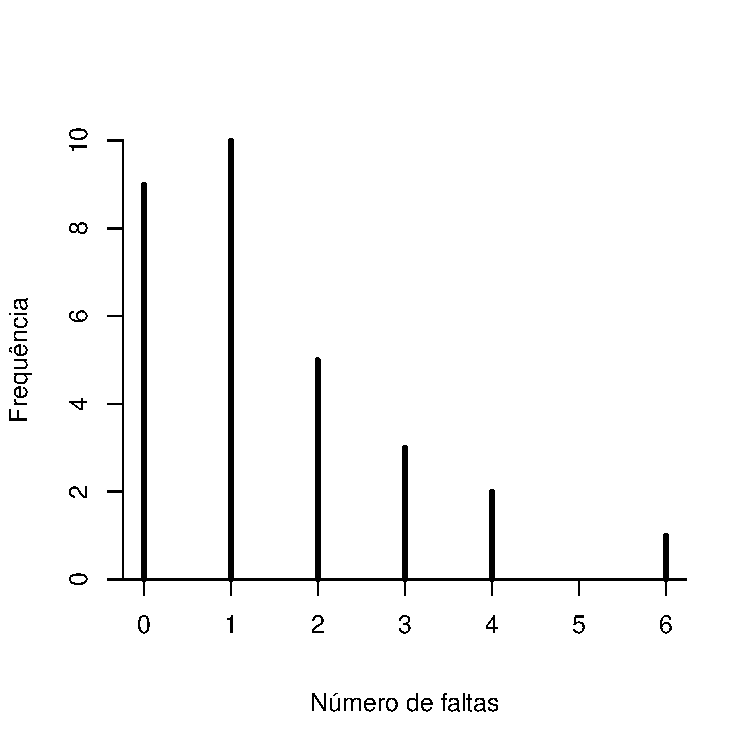
\includegraphics[trim=0 0cm 0 2cm, scale=0.8]{graflinhas.pdf}
\setlength{\abovecaptionskip}{0.5pt}
\caption{Diagrama de linhas do número de faltas}
\label{fig:graflinhas} % Unique label used for referencing the figure in-text
\end{figure}
	
\end{example}



\vspace{0,5cm}

Na Lista~\ref{lst:Rgraf4} são apresentados os comandos do software R para fazer o diagrama de linhas (Figura~\ref{fig:graflinhas}).  \\

\begin{scriptsize}
	\estiloR
	\begin{lstlisting}[caption={Comandos do software R}, label=lst:Rgraf4]
	# Entrando com os dados no R
	dados <- c(1, 3, 1, 1, 0, 1, 0, 1, 1, 0, 2, 2, 0, 0, 0, 1, 2, 1, 2, 0, 0, 1, 6, 4, 3, 3, 1, 2, 4, 0)
	 
	# Agrupando os dados em uma distribuição de frequências
	tab <- table(dados)
	
	# Plotando o diagrama de linhas
	plot(tab, xlab="Número de faltas", ylab="Frequência", lwd=3, axes=F, 
			frame.plot=F)
	axis(1,pos=0); axis(2); abline(h=0)
	
	\end{lstlisting}
\end{scriptsize}


\noindent {\bf Observações referentes à Lista~\ref{lst:Rgraf4}}: 

\begin{enumerate}[label=\alph*)]

\item dentro do comando \texttt{plot()} foram alterados alguns parâmetros gráficos. Foi usado o argumento \texttt{lwd=3} para aumentar a expessura das linhas; foi usado o argumento \texttt{axes=F} para omitir os eixos do gráfico; e foi usado o argumento \texttt{frame.plot=F} para omitir a "caixa" ao redor do gráfico;

\item o comando \texttt{axis(1,pos=0)} exibe o eixo das abcissas (eixo 1), e o argumento \texttt{pos=0} especifica que este eixo passará pela posição $y=0$;

\item o comando \texttt{axis(2)} exibe o eixo das ordenadas (eixo 2).
 
\end{enumerate}




%------------------------------------------------

\section{Histograma}

O histograma é utilizado para apresentar graficamente dados quantitativos contínuos agrupados em uma tabela de distribuição de frequências.

\subsubsection{Passos para construir um histograma} 


\begin{enumerate}

\item desenhe o sistema de eixos cartesianos;

\item no eixo das abscissas (eixo horizontal) apresente os limites das classes;

\item no eixo das ordenadas (eixo vertical) apresente uma escala de valores para as frequências;

\item desenhe barras com alturas iguais às frequências (ou às proporções ou porcentagens) das respectivas classes. As barras devem ser justapostas (não são separadas), a fim de evidenciar a natureza contínua da variável;

\item coloque legendas nos dois eixos e título na figura. \\

\end{enumerate}




\begin{example}

No Exemplo~\ref{exemp:distfreqquant2} foi construída uma tabela de distribuição de frequências para a variável  salário (Tabela~\ref{tab:distfreqquant2}). Esta tabela é apresentada novamente para facilitar a construção do histograma. \\

\begin{table}[h!]
	\begin{rBox}
	\captionsetup{labelformat=empty}
	\caption{\color{olivine!130}{Recordando a Tabela~\ref{tab:distfreqquant2}}} 
	\centering
	{\color{olivine!130}\begin{tabular}{l l l l}
	\toprule
	\textbf{Salários} & $\bm{f_i}$ & $\bm{fr_i}$ & $\bm{fp_i}$ \\
	\midrule
	\,\,\,$4,00 \vdash 8,00$  &  10  &  0,2778  &  27,78\% \\
	\,\,\,$8,00 \vdash 12,00$  &  12  &  0,3333  &  33,33\% \\
	$12,00 \vdash 16,00$  &  8  &  0,2222  &  22,22\% \\
	$16,00 \vdash 20,00$  &  5  &  0,1389  &  13,89\% \\
	$20,00 \vdash 24,00$  &  1  &  0,0278  &  2,78\% \\	
	\hline
	Total  &  36  &  1,0000  &  100,00\% \\
	\bottomrule
	\end{tabular}} \\
	\end{rBox}
\end{table}

Podemos representar essa distribuição de frequências por meio de um histograma (Figura~\ref{fig:grafhist}). \\ 

\begin{figure}[h!]
\centering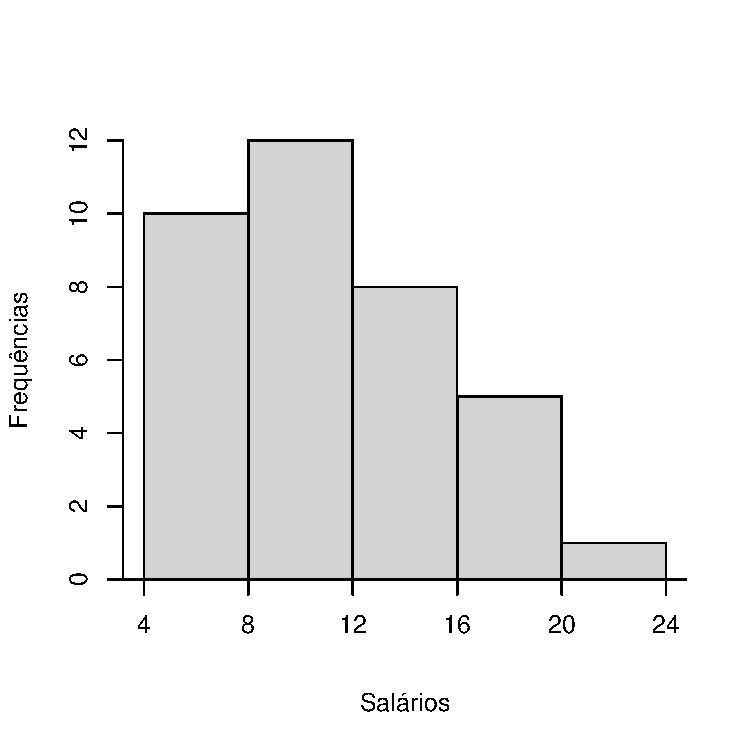
\includegraphics[trim=0 0cm 0 2.3cm, scale=0.8]{grafhist.pdf}
\setlength{\abovecaptionskip}{0.5pt}
\caption{Histograma dos salários}
\label{fig:grafhist} % Unique label used for referencing the figure in-text
\end{figure}

\end{example}


\vspace{0.3cm}

Na Lista~\ref{lst:Rgraf5} são apresentados os comandos do software R para fazer o histograma (Figura~\ref{fig:grafhist}).  \\


\begin{scriptsize}
	\estiloR
	\begin{lstlisting}[caption={Comandos do software R}, label=lst:Rgraf5]
	# Entrando com os dados no R
	dados <- c(5.73, 13.60, 13.23, 8.46, 17.26, 16.22, 8.74, 23.30, 7.39,
			11.06, 13.85, 8.12, 15.99, 10.76, 6.26, 9.80, 5.25, 9.77,
			19.40, 10.53, 11.59, 14.69, 8.95, 9.35, 4.56, 4.00, 9.13,
			14.71, 12.00, 7.59, 7.44, 6.66, 12.79, 18.75, 6.86, 16.61)
	 	
	# Plotando o histograma 
	hist(dados, breaks=c(4,8,12,16,20,24), xlab="Salários", ylab="Frequências",
			right=F, axes=F, col="lightgray", main="") 
	axis(1,c(4,8,12,16,20,24), pos=0); axis(2); abline(h=0)
	
	# Plotando um outro histograma sem especificar as classes
	hist(dados, xlab="Salários", ylab="Frequências", right=F, col="lightgray", main="") 

	\end{lstlisting}
\end{scriptsize}


\noindent {\bf Observações referentes à Lista~\ref{lst:Rgraf5}}: 

\begin{enumerate}[label=\alph*)]

\item no comando \texttt{hist()} os limites das classes foram especificados usando o argumento \texttt{breaks=c(4,8,12,16,20,24)};

\item o padrão do comando \texttt{hist()} é gerar intervalos fechados à direita. Para que sejam gerados intervalos abertos à direita deve-se utilizar o argumento \texttt{right=F};

\item o argumento \texttt{axes=F} faz com que os eixos ($x$ e $y$) não sejam gerados;

\item no argumento \texttt{col} pode ser especificada a cor do gráfico;

\item quando o argumento \texttt{breaks} não é informado dentro do comando \texttt{hist()} o software R gera classes usando um critério próprio, diferente do que foi visto neste material.

\end{enumerate}



%------------------------------------------------

\section{Polígono de frequências}

Dados quantitativos contínuos organizados em uma tabela de distribuição de frequências também podem ser apresentados em polígonos de frequências. 

O polígono de frequências utiliza os pontos médios das classes. Para calcular o ponto médio $(x_i)$ da classe $i$ basta calcular a média entre o limite inferior e o limite superior desta classe, ou seja, 

\begin{center}
$\displaystyle x_i=\frac{LI_i+LS_i}{2}$. \\
\end{center}


\subsubsection{Passos para construir um polígono de frequências}

\begin{enumerate}

	\item desenhe o sistema de eixos cartesianos;
	\item apresente os pontos médios das classes no eixo das abscissas (eixo horizontal);
	\item apresente as frequências no eixo das ordenadas (eixo vertical);
	\item marque pontos de coordenadas $(x_i,f_i)$ em que a coordenada $x_i$ é o ponto médio da classe e a coordenada $f_i$ é a frequência da classe;
	\item una os pontos por segmentos de reta;
	\item feche o polígono unindo os extremos da figura com o eixo horizontal. Utilize duas classes auxiliares, uma antes da primeira classe e outra depois da última classe, ambas com frequência zero, e utilize os pontos médios dessas classes auxiliares para fechar o polígono;
	\item coloque legendas nos dois eixos e título na figura. \\

\end{enumerate}



\begin{example}

No Exemplo~\ref{exemp:distfreqquant2} foi construída uma tabela de distribuição de frequências para a variável  salário (Tabela~\ref{tab:distfreqquant2}). Podemos representar essa distribuição de frequências por meio de um polígono de frequências (Figura~\ref{fig:grafpolifreq}). \\ 

\begin{figure}[h!]
\centering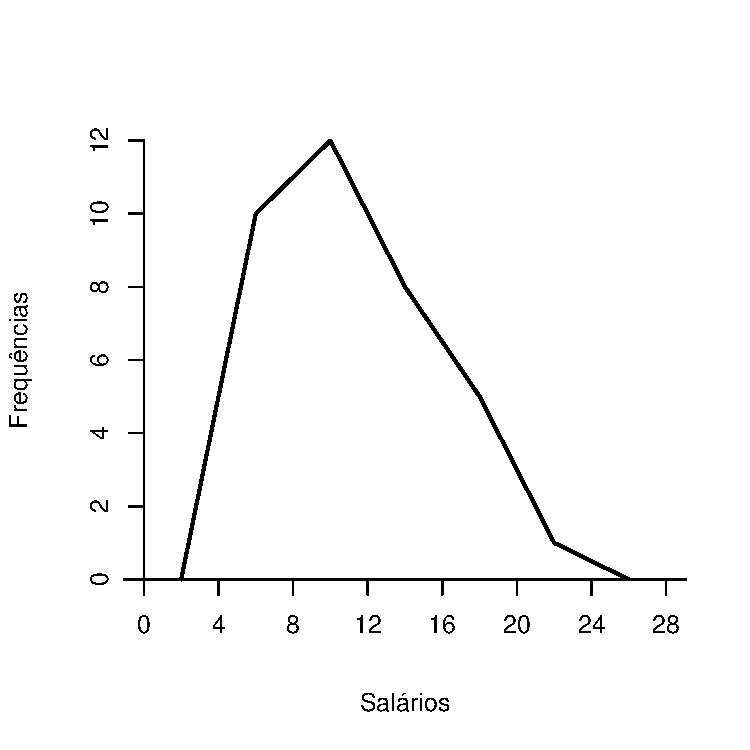
\includegraphics[trim=0 0cm 0 2cm, scale=0.8]{grafpolifreq.pdf}
\setlength{\abovecaptionskip}{0.5pt}
\caption{Polígono de frequências dos salários}
\label{fig:grafpolifreq} % Unique label used for referencing the figure in-text
\end{figure}

Para construir o polígono de frequências deve-se "criar" duas classes auxiliares, uma antes da primeira classe e outra depois da última classe, ambas com frequência zero, e obter os pontos médios dessas classes, como pode ser observado na Tabela~\ref{tab:auxpolifreq}.

\begin{table}[h!] 
	\caption{Tabela auxiliar para construção do polígono de frequências} 
	\label{tab:auxpolifreq}
	\centering
	\begin{tabular}{l c c}
	\toprule
	\textbf{Salários} & \textbf{Ponto médio} $\bm{(x_i)}$ & \textbf{Frequência} $\bm{(f_i)}$ \\
	\midrule
	\,\,\,\textcolor{ocre}{$\bm{0,00 \vdash 4,00$}}  & \textcolor{ocre}{\bf 2} &  \textcolor{ocre}{\bf 0}  \\
	\,\,\,$4,00 \vdash 8,00$  & 6 &  10  \\
	\,\,\,$8,00 \vdash 12,00$  & 10 &   12  \\
	$12,00 \vdash 16,00$  & 14 &   8  \\
	$16,00 \vdash 20,00$  & 18 &   5 \\
	$20,00 \vdash 24,00$  & 22 &   1 \\	
	\textcolor{ocre}{$\bm{24,00 \vdash 28,00$}}  & \textcolor{ocre}{\bf 26} &  \textcolor{ocre}{\bf 0}  \\
	\bottomrule
	\end{tabular} \\
\end{table}

Depois de construir a tabela auxiliar marque os pontos $(x_i, f_i)$ (Figura~\ref{fig:grafpolifreq3}A) e depois ligue os pontos usando segmentos de retas (Figura~\ref{fig:grafpolifreq3}B). \\


\begin{figure}[h!]
\centering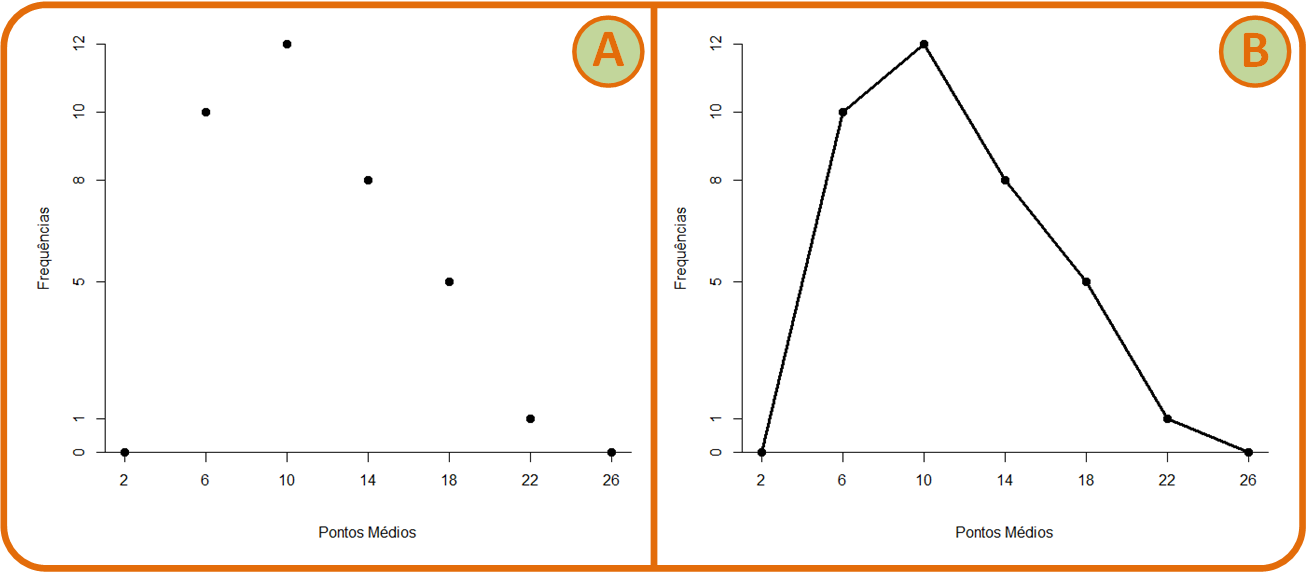
\includegraphics[trim=0 0cm 0 0cm, scale=0.54]{grafpolifreq3.png}
\setlength{\abovecaptionskip}{0.5pt}
\caption{Construção do polígono de frequências}
\label{fig:grafpolifreq3} % Unique label used for referencing the figure in-text
\end{figure}

\end{example}

\vspace{0.5cm}

Na Lista~\ref{lst:Rgraf6} são apresentados os comandos do software R para fazer o polígono de frequências (Figura~\ref{fig:grafpolifreq}).  \\


\begin{scriptsize}
	\estiloR
	\begin{lstlisting}[caption={Comandos do software R}, label=lst:Rgraf6]
	# Entrando com os dados no R
	dados <- c(5.73, 13.60, 13.23, 8.46, 17.26, 16.22, 8.74, 23.30, 7.39,
			11.06, 13.85, 8.12, 15.99, 10.76, 6.26, 9.80, 5.25, 9.77,
			19.40, 10.53, 11.59, 14.69, 8.95, 9.35, 4.56, 4.00, 9.13,
			14.71, 12.00, 7.59, 7.44, 6.66, 12.79, 18.75, 6.86, 16.61)

	# Agrupando os dados em classes 
	hg <- hist(dados, breaks=c(4,8,12,16,20,24), plot=F, right=F)
	
	# Mostrando o objeto hg
	hg
	
	# Amplitude das classes
	c <- diff(hg$breaks[1:2])
	
	# Pontos médios das classes (com classes auxiliares)
	pm = c(hg$mids[1]-c, hg$mids, hg$mids[length(hg$mids)]+c)
	
	# Frequências das classes (classes auxiliares freq. zero)
	freq <- c(0, hg$counts, 0)
	
	# Plotando o polígono de frequências
	plot(pm, freq, type="l", lwd=2, bty="l", xlab="Salários", 
			ylab="Frequências", main="", axes=F, xlim=c(0,max(hg$breaks)+c))
	axis(1, seq(0,max(hg$breaks)+c,c), pos=0); axis(2, pos=0); abline(h=0)

	\end{lstlisting}
\end{scriptsize}

\vspace{0.3cm}

\noindent {\bf Observações referentes à Lista~\ref{lst:Rgraf6}}: 

\begin{enumerate}[label=\alph*)]

\item primeiramente foi criado um objeto (\texttt{hg}) contendo a distribuição de frequências. Esse objeto é do tipo lista e na saída desse objeto são mostradas várias estruturas de dados. Por exemplo, em \texttt{hg\$breaks} são dados os limites das classes, em \texttt{hg\$counts} são dadas as frequências das classes e em \texttt{hg\$mids} são dados os pontos médios das classes, etc;

\item a amplitude das classes \texttt{(c)} foi obtida pela diferença (comando \texttt{diff()}) entre os dois primeiros limites das classes, ou seja, \texttt{diff(hg\$breaks[1:2])};

\item os pontos médios das classes são obtidos no objeto \texttt{hg} em \texttt{\$mids}. Para obter os pontos médios das classes auxiliares a amplitude das classes (\texttt{c}) foi subtraída da primeira classe (\texttt{hg\$mids[1]-c}) e somada à última classe (\texttt{hg\$mids[length(hg\$mids)]+c});

\item foi atribuído valor zero às frequências das classes auxiliares e foram mantidas as frequências das classes originais usando o comando \texttt{c(0, hg\$counts, 0)} para criar o objeto \texttt{freq}. \\

\end{enumerate}


Também é possível apresentar o histograma e o polígono de frequências sobrepostos em um mesmo gráfico. Na Lista~\ref{lst:Rgraf6.2} são apresentados os comandos do software R para fazer o histograma e o polígono de frequências juntos (Figura~\ref{fig:grafhistpoli}).  \\

\begin{figure}[h!]
\centering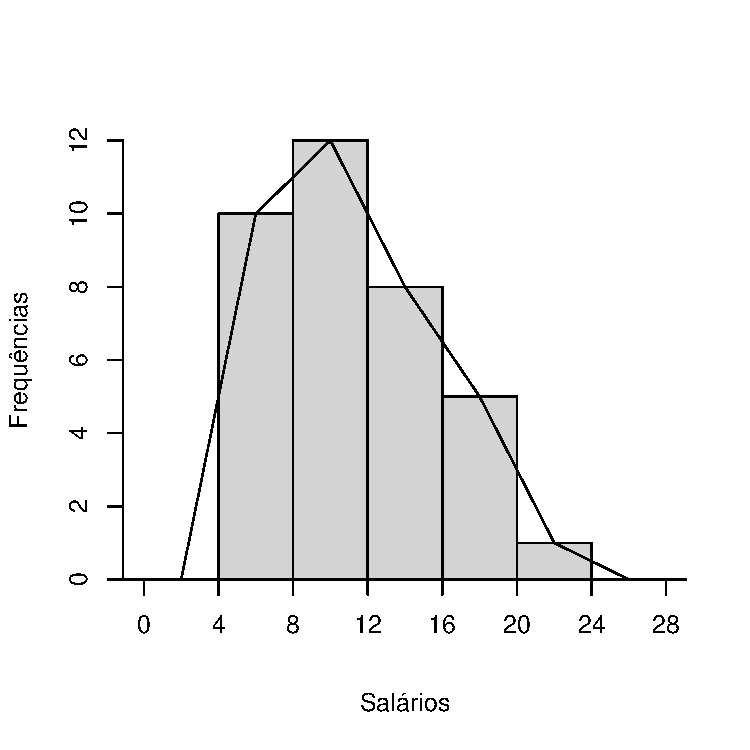
\includegraphics[trim=0 0cm 0 2cm, scale=0.8]{grafhistpoli.pdf}
\setlength{\abovecaptionskip}{0.5pt}
\caption{Histograma com polígono de frequências}
\label{fig:grafhistpoli} % Unique label used for referencing the figure in-text
\end{figure}


\begin{scriptsize}
	\estiloR
	\begin{lstlisting}[caption={Comandos do software R}, label=lst:Rgraf6.2]
	# Entrando com os dados no R
	dados <- c(5.73, 13.60, 13.23, 8.46, 17.26, 16.22, 8.74, 23.30, 7.39,
			11.06, 13.85, 8.12, 15.99, 10.76, 6.26, 9.80, 5.25, 9.77,
			19.40, 10.53, 11.59, 14.69, 8.95, 9.35, 4.56, 4.00, 9.13,
			14.71, 12.00, 7.59, 7.44, 6.66, 12.79, 18.75, 6.86, 16.61)
	 	
	# Pacote agricolae
	library(agricolae)
	
	# Histograma (deve-se criar um objeto)
	histograma <- hist(dados, breaks=c(4,8,12,16,20,24), xlim=c(0, 28), 
			xlab="Salários", ylab="Frequências", right=F, axes=F, 
			col="lightgray", main="") 
	axis(1,c(0,4,8,12,16,20,24,28), pos=0); axis(2); abline(h=0)
	
	# Polígono de frequências sobreposto ao histograma
	polygon.freq(histograma)	


	\end{lstlisting}
\end{scriptsize}





%------------------------------------------------

\section{Ramo e folhas}

Um "gráfico" simples para resumir um conjunto de dados quantitativos com poucas observações é o ramo-e-folhas. Uma vantagem do ramo-e-folhas é que ele explicita os dados.
Não existe uma regra fixa para construir o ramo-e-folhas, mas a idéia básica é dividir cada observação em duas partes: a primeira, o ramo, é colocada à esquerda de uma linha vertical, a segunda, as folhas, é colocada à direita. 

O ramo e as folhas podem representar quaisquer grandezas: unidades e decimais, dezenas e unidades, centenas e dezenas, etc. Por esse motivo é aconselhável que o ramo-e-folhas tenha uma legenda para facilitar sua interpretação. \\


\begin{example}

	Considere as idades, em meses, de 30 animais:
	
	\begin{center}
	\begin{tabular}{c c c c c c c c c c c c c c c}
	\hline
	82 & 72 & 22 & 44 & 30 & 41 & 32 & 78 & 43 & 22 & 65 & 56 & 42 & 65 & 61 \\
	61 & 71 & 88 & 52 & 55 & 101 & 24 & 62 & 50 & 68 & 80 & 55 & 12 & 18 & 32 \\
	\hline
	\end{tabular}
	\end{center}
	

	Os dados podem ser organizados, separando-os pela dezenas, uma em cada linha:
	
	
	\begin{center}
	\begin{tabular}{c c c c c c}
	\hline
   	12 & 18 &  &  &  & \\
   	22 & 22 & 24  &  &  & \\
   	30 & 32 & 32 &  &  & \\
   	41 & 42 & 43 & 44 &  & \\
   	50 & 52 & 55 & 55 & 56 &  \\
   	61 & 61 & 62 & 65 & 65 & 68 \\
   	71 & 72 & 78 &  &  & \\
   	80 & 82 & 88 &  &  & \\
  	101 &  &  &  &  & \\
	\hline
	\end{tabular}
	\end{center}
	
	
Os dados em cada linha tem as dezenas em comum, logo pode-se colocar as dezenas em evidência, separando-as das unidades por uma linha vertical. Ao dispor os dados dessa forma, é construído um diagrama de ramo-e-folhas (Figura~\ref{fig:grafrf1}).
	
	
\begin{figure}[h!]
	\begin{center}
	\fbox{
	{\bf \begin{tabular}{c c c c | c c c c c c}
   	& & & 1 & 2 & 8 &  &  &  & \\
   	& & & 2 & 2 & 2 & 4  &  & \\
   	& & & 3 & 0 & 2 & 2  &  & \\
   	& & & 4 & 1 & 2 & 3 & 4 & \\
   	& & & 5 & 0 & 2 & 5 & 5 & 6 &  \\
   	& & & 6 & 1 & 1 & 2 & 5 & 5 & 8  \\
   	& & & 7 & 1 & 2 & 8 &  &  &  \\
   	& & & 8 & 0 & 2 & 8 &  &  & \\
   	& & & 9 & & & & & \\
  	& & & 10& 1 &  &  &  & \\
	\end{tabular}}
	\begin{tabular}{r r r r r}
	\\
	\\
	\\
	\\
	\\
	\\
	\\
	\\
	\\
	\\
	\\
	\\
	\\
	& & & {\bf Legenda:} &  1\,{\bf |}\,2\,=\,12 meses \, \\
	& & & &  10\,{\bf |}\,1\,=\,101 meses \\
	\end{tabular}
	}
	\end{center}
	\setlength{\abovecaptionskip}{0.5pt}
\caption{Ramo-e-folhas das idades}
\label{fig:grafrf1} % Unique label used for referencing the figure in-text
\end{figure}

\end{example}

\vspace{0.5cm}

Na Lista~\ref{lst:Rgraf7} são apresentados os comandos do software R para fazer o ramo-e-folhas das idades.  \\


\begin{scriptsize}
	\estiloR
	\begin{lstlisting}[caption={Comandos do software R}, label=lst:Rgraf7]
	# Entrando com os dados no R
	dados <- c(82, 72, 22, 44, 30, 41, 32, 78, 43, 22, 65, 56, 42, 65, 61, 
		61, 71, 88, 52, 55, 101, 24, 62, 50, 68, 80, 55, 12, 18, 32)

	# Ramo-e-folhas
	stem(dados)

	\end{lstlisting}
\end{scriptsize}



\begin{example}

	Considere os dados brutos dos salários (em x sal. mín.) de 36 indivíduos:
	
	\begin{center}
	\begin{tabular}{c c c c c c c c c}
	\hline
	5,73  &  13,60  &  13,23  &  8,46  &  17,26  &  16,22  &  8,74  &  23,30  &  7,39 \\
	11,06  &  13,85  &  8,12  &  15,99  &  10,76  &  6,26  &  9,80  &  5,25  &  9,77 \\
	19,40  &  10,53  &  11,59  &  14,69  &  8,95  &  9,35  &  4,56  &  4,00  &  9,13 \\
	14,71  &  12,00  &  7,59  &  7,44  &  6,66  &  12,79  &  18,75  &  6,86  &  16,61 \\
	\hline
	\end{tabular}
	\end{center}
	
	Esses dados podem ser representados em um ramo-e-folhas em que a unidade representa os ramos e a parte decimal representa as folhas (Figura~\ref{fig:grafrf2}). {\bf Observação}: deve-se arredondar os dados para uma casa decimal para que cada valor à direita da linha vertical represente uma folha (cada número seja referente a um dado).


\begin{figure}[h!]
	\begin{center}
	\fbox{
	{\bf \begin{tabular}{c c c c | c c c c c}
   & & & 4 & 0 & 6 \\
   & & & 5 & 3 & 7 \\
   & & & 6 & 3 & 7 & 9 \\
   & & & 7 & 4 & 4 & 6 \\
   & & & 8 & 1 & 5 & 7 \\
   & & & 9 & 0 & 1 & 4 & 8 & 8 \\
  & & & 10 & 5 & 8 \\
  & & & 11 & 1 & 6 \\
  & & & 12 & 0 & 8 \\
  & & & 13 & 2 & 6 & 9 \\
  & & & 14 & 7 & 7 \\
  & & & 15 & \\
  & & & 16 & 0 & 2 & 6 \\
  & & & 17 & 3 \\
  & & & 18 & 8 \\
  & & & 19 & 4 \\
  & & & 20 & \\
  & & & 21 & \\
  & & & 22 & \\
  & & & 23 & 3 \\
	\end{tabular}}
	\begin{tabular}{r r r r r}
	\\
	\\
	\\
	\\
	\\
	\\
	\\
	\\
	\\
	\\
	\\
	\\
	\\
	\\
	\\
	\\
	\\
	\\
	\\
	\\
	\\
	\\
	\\
	& & & {\bf Legenda:} &  4\,{\bf |}\,0\,=\,4,0 salários \, \\
	& & & &  23\,{\bf |}\,3\,=\,23,3 salários \\
	\end{tabular}
	}
	\end{center}
	\setlength{\abovecaptionskip}{0.5pt}
\caption{Ramo-e-folhas dos salários}
\label{fig:grafrf2} % Unique label used for referencing the figure in-text
\end{figure}


\end{example}

\vspace{0.5cm}




Na Lista~\ref{lst:Rgraf8} são apresentados os comandos do software R para fazer o ramo-e-folhas para os dados de salários.  \\

\vspace{3cm}


\begin{scriptsize}
	\estiloR
	\begin{lstlisting}[caption={Comandos do software R}, label=lst:Rgraf8]
	# Entrando com os dados no R
	dados <- c(5.73, 13.60, 13.23, 8.46, 17.26, 16.22, 8.74, 23.30, 7.39,
			11.06, 13.85, 8.12, 15.99, 10.76, 6.26, 9.80, 5.25, 9.77,
			19.40, 10.53, 11.59, 14.69, 8.95, 9.35, 4.56, 4.00, 9.13,
			14.71, 12.00, 7.59, 7.44, 6.66, 12.79, 18.75, 6.86, 16.61)
	
	# Arredondando os dados para uma casa decimal e ordenando(OPCIONAL)
	sort(round(dados,1))
	
	# Ramo-e-folhas
	stem(dados, scale=2)

	\end{lstlisting}
\end{scriptsize}

\noindent {\bf Observação}: Na Lista~\ref{lst:Rgraf8}, no comando \texttt{stem()}, o parâmetro \texttt{scale} foi alterado para \texttt{scale=2} para que fossem exibidos todos os valores do ramo (de 4 à 23). \\


%------------------------------------------------

\section{Gráfico de Série Temporal}

Este gráfico serve para representar uma série temporal, ou seja, dados coletados em diferentes momentos do tempo. 

\subsubsection{Passos para construir um gráfico de série temporal}

\begin{enumerate}

\item desenhe o sistema de eixos cartesianos;

\item anote os períodos de tempo da variável estudada no eixo das abscissas (eixo horizontal);

\item escreva as frequências ou taxas no eixo das ordenadas (eixo vertical), obedecendo uma escala;

\item marque pontos de coordenadas $(x_i; f_i)$ em que a coordenada $x_i$ representa o tempo no qual foi registrada a informação e a coordenada $f_i$ é a frequência ou taxa observada no respectivo tempo;

\item una os pontos por segmentos de reta;

\item coloque legenda nos dois eixos (nomes dos eixos) e título na figura;

\item no caso de existir mais de uma série, coloque uma legenda no gráfico para identificar cada uma das séries. \\

\end{enumerate}


\begin{example}

A Tabela~\ref{tab:taxaocup} apresenta informações sobre a taxa de ocupação da rede hoteleira dos municípios de Búzios e Petrópolis, no estado do Rio de Janeiro, no período de 2000 a 2008. \\	

\begin{table}[h]
	\caption{Taxa de ocupação da rede hoteleira}
	\label{tab:taxaocup} 
	%\vspace{0.1cm}
	\centering
	\begin{tabular}{c c c}
	\toprule
	\textbf{Ano} & \textbf{Búzios} & \textbf{Petrópolis}\\
	\midrule
	2000 & 72.8 & 60.6 \\
	2001 & 66.2 & 53.7 \\
	2002 & 69.2 & 55.3 \\
	2003 & 65.9 & 56.7 \\
	2004 & 62.4 & 56.4 \\
	2005 & 67.8 & 57.8 \\
	2006 & 61.3 & 57.5 \\
	2007 & 68.5 & 59.8 \\
	2008 & 70.4 & 63.3 \\
	\bottomrule
	\end{tabular} \\
\end{table}

Podemos representar graficamente esta tabela como um gráfico de duas séries temporais (Figura~\ref{fig:grafseriestemp}).

\begin{figure}[h!]
\centering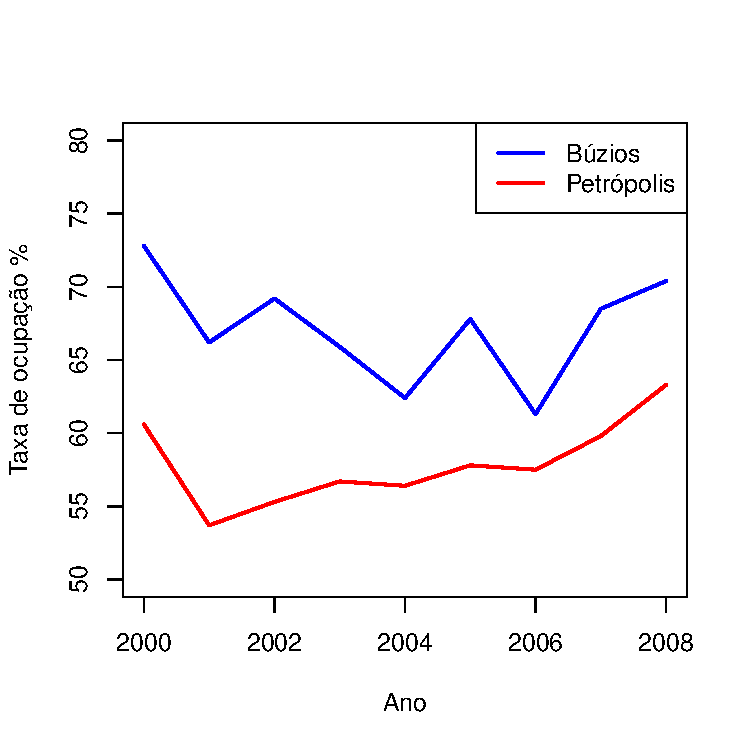
\includegraphics[trim=0 0cm 0 2cm, scale=0.8]{grafseriestemp.pdf}
\setlength{\abovecaptionskip}{0.5pt}
\caption{Taxa de ocupação hoteleira}
\label{fig:grafseriestemp} % Unique label used for referencing the figure in-text
\end{figure}

\end{example}

\vspace{0,3cm}

Na Lista~\ref{lst:Rgraf9} são apresentados os comandos do software R para fazer o gráfico de séries temporais (Figura~\ref{fig:grafseriestemp}). \\


\begin{scriptsize}
	\estiloR
	\begin{lstlisting}[caption={Comandos do software R}, label=lst:Rgraf9]
	# Entrando com os dados
	Ano <- 2000:2008
	Buzios <- c(72.8, 66.2, 69.2, 65.9, 62.4, 67.8, 61.3, 68.5, 70.4)
	Petropolis <- c(60.6, 53.7, 55.3, 56.7, 56.4, 57.8, 57.5, 59.8, 63.3)
	
	# Gerando o gráfico de séries temporais de Búzios
	plot(Ano, Buzios, type="l", xlab="Ano", ylab="Taxa de ocupação %", 
	xlim=c(2000,2008), ylim=c(50,80), col="blue", lwd=2, pch=16)
	
	# Sobrepondo a série de Petropólis ao gráfico de Búzios gerado anteriormente
	lines(Ano, Petropolis, col="red", lwd=2) 
	
	# Adicionando a legenda
	legend("topright", c("Búzios","Petrópolis"), lwd=2, col=c("blue","red"))

	\end{lstlisting}
\end{scriptsize}


\noindent {\bf Observações referentes à Lista~\ref{lst:Rgraf9}}:

\begin{enumerate}[label=\alph*)]

\item Foi criado o objeto ano para representar o período de tempo no qual foram coletadas as informações;

\item Foram criados os objetos Buzios e Petropolis contendo as taxas de ocupação da rede hoteleira observadas em cada ano de acordo com cada município;

\item No comando \texttt{plot()} é especificado o objeto relativo à primeira série estudada (Búzios);

\item O argumento \texttt{type="l"} indica que o gráfico será realizado no formato de uma linha;

\item O argumento \texttt{lwd=2} indica a espessura da linha do gráfico;

\item No comando \texttt{lines()} é especificado o objeto relativo à segunda série estudada (Petrópolis);

\item No comando \texttt{legend()} são especificados: o local do gráfico (coordenadas) no qual a legenda será plotada, o vetor com os nomes de cada série, a espessura e as cores das linhas.

\end{enumerate}


%----------------------------------------------------------------------------------------
%	CHAPTER 7
%----------------------------------------------------------------------------------------

\chapterimage{chapter_head_3.pdf} % Chapter heading image

\chapter{Medidas de posição}

%------------------------------------------------

\section{Introdução}
Foi visto nas seções anteriores que o resumo de dados por meio de tabelas de distribuição de frequências e gráficos
fornece muito mais informação sobre o comportamento de uma variável do que o próprio conjunto original de dados (dados brutos). Muitas vezes, é necessário resumir ainda mais os dados, apresentando algumas medidas que sejam capazes de resumir aspectos importantes da distribuição da variável de interesse. Usualmente, emprega-se uma das seguintes {\itshape medidas de posição}: média, mediana ou moda. Essas medidas de posição também são denominadas de {\itshape medidas de tendência central}.

\section{Somatório}
\vspace{0,3cm}
\subsection{Variáveis e índices}
\vspace{0,3cm}

O símbolo $x_i$ (leia $x$ índice $i$) representa qualquer um dos $n$ valores $x_1, x_2, ..., x_n$ assumidos por uma variável aleatória $X$ no conjunto de dados. A letra $i$, usada como índice, indica a "posição" (de $1$ a $n$) do elemento $x$ no conjunto de dados. Assim, $x_1$ é o elemento que ocupa a primeira posição na amostra, $x_2$ é o elemento que ocupa a segunda posição na amostra e assim consecutivamente até $x_n$ que é o elemento que ocupa a 
$n$-ésima posição na amostra.\\



\begin{example} \label{exemp:varIndices}
Se for considerada uma amostra de tamanho $n=3$ pessoas e se $X$ representa uma variável relativa ao peso, em $kg$, então uma possibilidade de resultados é:

\begin{center}
	$50,5$, \, $64,3$ \, e \, $72,6$
\end{center}

Logo, $x_1=50,5$, $x_2=64,3$ e $x_3=72,6$.
\end{example}
\vspace{0.5cm}


%------------------------------------------------

\subsection{Notação de somatório}
\vspace{0,3cm}

Para representarmos a soma de $n$ variáveis aleatórias podemos utilizar o símbolo $\Sigma$, letra grega maiúscula sigma (Equação~\ref{eq:somatorio}).

\begin{eBox}
\vspace{-0.5cm}
\begin{equation} \label{eq:somatorio}
		\displaystyle 	\sum_{i=1}^{n}x_i=x_1+x_2+...+x_n
\end{equation}
\end{eBox}

\noindent ou seja, a soma $x_1+x_2+...+x_n$ pode ser representada por $\displaystyle \sum_{i=1}^{n}x_i$.  Lê-se somatório de $x_i$ para $i$ variando de $1$ até $n$.\\



\begin{example} \label{exemp:somatorio}
	Considere os dados de peso de $n=3$ pessoas: \{$50,5$, \, $64,3$ \, e \, $72,6$\}.\\

	O somatório desses dados é calculado por:

	\begin{ceqn}
	\begin{align*}
	\centering
	\sum_{i=1}^{3}x_i 	
	&= x_1+x_2+x_3 \\
    &= 50,5+64,3+72,6 \\
    &= 187,4
	\end{align*}
	\end{ceqn}

	
\end{example}
\vspace{0.5cm}


Na Lista~\ref{lst:Rsoma1} são apresentados os comandos do software R para realizar a entrada dos dados e o cálculo do somatório do Exemplo~\ref{exemp:somatorio}.\\

\begin{scriptsize}
	\estiloR
	\begin{lstlisting}[caption={Comandos do software R}, label=lst:Rsoma1]
	# Entrando com os dados no R
	x <- c(50.5, 64.3, 72.6)
	
	# Mostrando os dados armazenados
	x

	# Somatório de x
	sum(x)

	\end{lstlisting}
\end{scriptsize}


Na notação de somatório a variação do índice $i$ pode não ir de $1$ a $n$ mas estar em qualquer subintervalo desses limites como pode ser observado no Exemplo~\ref{exemp:somatorioIndicesDiferentes}.\\


\begin{example} \label{exemp:somatorioIndicesDiferentes}

	Seja a amostra  $X=\{6,\,\,  5,\,\,  2,\,\,  8,\,\,  3,\,\,  7\}$ de tamanho $n=6$. Determine: \\

	\noindent \hspace{0.4cm} a) \, $\displaystyle \sum_{i=1}^{n}{x_i}$ 
	                  \qquad b) \, $\displaystyle \sum_{i=2}^{5}{x_i}$. \\ \\
	
	\noindent \hspace{0.3cm}{\small\bf\sffamily Solução} \\
	
	\begin{enumerate}[label=\alph*)]
	
	\item $\displaystyle \sum_{i=1}^{n}{x_i} \ = \ \sum_{i=1}^{6}{x_i} \ = \ x_1+x_2+x_3+x_4+x_5+x_6 \ = \ 6+5+2+8+3+7 \ = \ 31 $.
	\item $\displaystyle \sum_{i=2}^{5}{x_i} \ = \ x_2+x_3+x_4+x_5 \ = \ 5+2+8+3 \ = \ 18 $.
	\end{enumerate}
	
\end{example}
\vspace{0.3cm}

%------------------------------------------------

\subsection{Propriedades de somatório}
\vspace{0,3cm}

\begin{enumerate}[label=\alph*)]
	\item $\displaystyle \sum_{i=1}^{n}{ax_i} \ = \ ax_1+ax_2+...+ax_n \ = \ a\displaystyle \sum_{i=1}^{n}x_i $
	
	\item $\displaystyle \sum_{i=1}^{n}{x_i y_i} \ = \ x_1 y_1+x_2 y_2+...+x_n y_n \ {\neq} \ 
	\left(\sum_{i=1}^{n}x_i\right) \left(\sum_{i=1}^{n}y_i\right) $
	
	\item $\displaystyle \sum_{i=1}^{n}{\left( ax_i+by_i \right)} \ = \ ax_1+by_1+ax_2+by_2+...+ax_n+by_n  \ = \ 
	a\sum_{i=1}^{n}x_i + b\sum_{i=1}^{n}y_i $
	
	\item $\displaystyle \sum_{i=1}^{n}{x_i^2} \ = \ x_1^2+x_2^2+...+x_n^2 \ {\neq} \ 
	\left(\sum_{i=1}^{n}x_i\right)^2 $
	
	\item $\displaystyle \sum_{i=1}^{n}k \ = \ \underbrace{k+k+...+k}_{\mbox{n vezes}} \ = \ nk $\\
	
\end{enumerate}

em que $a$, $b$ e $k$ são constantes.\\


Utilize as propriedades de somatório apresentadas anteriormente para fazer o Exercício~\ref{exerc:somatorio}. \\


\begin{exercise} \label{exerc:somatorio}
	Sejam as amostras de tamanho $n=5$ dadas por 

	\begin{center}
	$X=\{2,\,\, 7,\,\, 4,\,\, 3,\,\, 2\}$ \, e \, $Y=\{1,\,\, 2,\,\, 3,\,\, 6,\,\, 5\}$.
	\end{center}	
	
	Determine: \\
	
	\noindent \hspace{0.4cm} a) \, $\displaystyle \sum_{i=1}^{n}{x_i}$ 
	                  \qquad b) \, $\displaystyle \sum_{i=1}^{n}{y_i}$ 
	                  \qquad c) \, $\displaystyle \sum_{i=1}^{n}{x_i y_i}$ 
	                  \qquad d) \, $\displaystyle \sum_{i=1}^{n}{(3x_i+2y_i)}$ 
	                  \qquad e) \, $\displaystyle \sum_{i=1}^{n}{x_i^2}$ \\ \\
	                  
	\noindent \hspace{0.4cm} f) \, $\displaystyle \left(\sum_{i=1}^{n}{x_i}\right)^2$ 
	                  \qquad g) \, $\displaystyle \sum_{i=1}^{n}{y_i^2}+\left(\sum_{i=1}^{n}{y_i}\right)^2$
	 
\end{exercise}
\vspace{0.3cm}


Na Lista~\ref{lst:Rsoma2} são apresentados os comandos do software R para fazer os cálculos dos somatórios solicitados no Exercício~\ref{exerc:somatorio}. Use as saídas do R como gabarito para este exercício.\\

\begin{scriptsize}
	\estiloR
	\begin{lstlisting}[caption={Comandos do software R}, label=lst:Rsoma2]
	# Entrando com os dados no R
	x <- c(2,7,4,3,2)
	y <- c(1,2,3,6,5)
	
	# Item (a)
	sum(x)
	
	# Item (b)
	sum(y)
	
	# Item (c)
	sum(x*y)

	# Item (d)
	sum(3*x+2*y)
	
	# Item (e)
	sum(x^2)
	
	# Item (f)
	(sum(x))^2
	
	# Item (g)
	sum(y^2)+(sum(y))^2

	\end{lstlisting}
\end{scriptsize}


%------------------------------------------------

\section{Média aritmética}

Dentre as medidas de posição a mais utilizada é a média. Ela é resultante da soma de todas as observações dividida pelo total de observações.


\subsection{Média aritmética (para dados brutos)}

Se $x_1, x_2, ..., x_n$ são $n$ valores de uma variável quantitativa $X$, então a média aritmética (ou simplesmente média) de $X$ é dada pela Equação~\ref{eq:mediadadosbrutos}.

\begin{eBox}
\vspace{-0.5cm}
\begin{equation} \label{eq:mediadadosbrutos}
	\bar{x}=\frac{\displaystyle \sum_{i=1}^{n}{x_i}}{n}
\end{equation}
\end{eBox}

\vspace{0.3cm}

Lê-se "$x$ barra" é igual ao somatório de $x$ dividido por $n$. \\


\begin{example} \label{exemp:media1}

Considere os dados brutos dos salários (em x sal. mín.) de 36 indivíduos:
	
	\begin{center} \label{dadosbrutossalarios}
	\begin{tabular}{c c c c c c c c c}
	\hline
	5,73  &  13,60  &  13,23  &  8,46  &  17,26  &  16,22  &  8,74  &  23,30  &  7,39 \\
	11,06  &  13,85  &  8,12  &  15,99  &  10,76  &  6,26  &  9,80  &  5,25  &  9,77 \\
	19,40  &  10,53  &  11,59  &  14,69  &  8,95  &  9,35  &  4,56  &  4,00  &  9,13 \\
	14,71  &  12,00  &  7,59  &  7,44  &  6,66  &  12,79  &  18,75  &  6,86  &  16,61 \\
	\hline
	\end{tabular}
	\end{center}
	
A média dos salários (ou salário médio) é calculada por: \\

\begin{center}
$\displaystyle \bar{x}=\frac{\sum{x_i}}{n}=\frac{5,73+13,60+...+16,61}{36}=\frac{400,4}{36}=11,12$ salários mínimos.
\end{center}


\end{example}

\vspace{0,3cm}

Na Lista~\ref{lst:Rmedia1} são apresentados os comandos do software R para calcular a média do Exemplo~\ref{exemp:media1}. O comando do R usado para calcular a média é o comando \texttt{mean()}.\\

\begin{scriptsize}
	\estiloR
	\begin{lstlisting}[caption={Comandos do software R}, label=lst:Rmedia1]
	# Entrando com os dados no R
	dados <- c(5.73, 13.60, 13.23, 8.46, 17.26, 16.22, 8.74, 23.30, 7.39,
			11.06, 13.85, 8.12, 15.99, 10.76, 6.26, 9.80, 5.25, 9.77,
			19.40, 10.53, 11.59, 14.69, 8.95, 9.35, 4.56, 4.00, 9.13,
			14.71, 12.00, 7.59, 7.44, 6.66, 12.79, 18.75, 6.86, 16.61)

	# Média
	mean(dados)

	\end{lstlisting}
\end{scriptsize}


\subsection{Média aritmética (para dados agrupados)}
%\vspace{0.3cm}

Quando os dados são discretos e em grande número, pode haver repetição de valores. Nesses casos, é razoável agrupar os dados em uma tabela de distribuição de frequências. Veja a Tabela~\ref{tab:distfreqdisc}. 

\begin{table}[H]
	\caption{Distribuição de frequências para dados discretos}
	\label{tab:distfreqdisc} 
	\vspace{-0.1cm}
	\centering
	\begin{tabular}{c c}
	\toprule
	\textbf{Valores da variável ($\bm{x_i}$)} & \textbf{Frequências ($\bm{f_i}$)}\\
	\midrule
	$x_1$ & $f_1$ \\
	$x_2$ & $f_2$ \\
	\vdots & \vdots \\
	$x_k$ & $f_k$ \\
	\midrule
	Total & $\sum{f_i}$ \\
	\bottomrule
	\end{tabular} \\
\end{table}


A média aritmética de dados agrupados em uma tabela de distribuição de frequências é dada pela Equação~\ref{eq:mediadadosagrupados}.

\begin{eBox}
\vspace{-0.5cm}
\begin{equation} \label{eq:mediadadosagrupados}
	\bar{x}=\frac{\displaystyle \sum_{i=1}^{n}{x_i f_i}}{\displaystyle \sum_{i=1}^{n}{f_i}}
\end{equation}
\end{eBox}

\vspace{0.3cm}

\noindent {\bf Observação}: Note que $x_i f_i=\underbrace{x_i+x_i+...+x_i}_{f_i \, \, \mbox{vezes}}$, \, então $\displaystyle \sum_{i=1}^{n}{x_i f_i}=x_1 f_1+x_2 f_2+...+x_k f_k$ \, é igual ao somatório de todos os dados, e, $\displaystyle \sum_{i=1}^{n}{f_i}=f_1+f_2+...+f_k=n$, ou seja, a soma de todas as frequências é igual ao número de elementos do conjunto de dados. \\


\begin{example} \label{exemp:media2}

Considere a tabela de distribuição de frequências do número de filhos de vinte funcionários (Tabela~\ref{tab:distnumfilhos}).

	\begin{table}[h]
	\caption{Distribuição de frequências do número de filhos de vinte funcionários}
	\label{tab:distnumfilhos} 
	\vspace{-0.1cm}
	\centering
	\begin{tabular}{c c c}
	\toprule
	\textbf{Número de filhos} ($\bm{x_i}$) & \textbf{Frequências} ($\bm{f_i}$) & \textbf{Produtos} ($\bm{x_i f_i}$) \\
	\midrule
	0 & 6 & $0 \times 6 = 0$ \\
	1 & 8 & $1 \times 8 = 8$ \\
	2 & 4 & $2 \times 4 = 8$ \\
	3 & 1 & $3 \times 1 = 3$ \\
	4 & 0 & $4 \times 0 = 0$ \\
	5 & 1 & $5 \times 1 = 5$ \\
	\hline
	Total & $\sum{f_i}=20$ & $\sum{x_i f_i}=24$\\
	\bottomrule
	\end{tabular} \\
	\end{table}
	
A média do número de filhos é calculada por:

\begin{center}
$\displaystyle \bar{x}=\frac{\sum{x_i f_i}}{\sum{f_i}}=\frac{24}{20}=1,2$ filhos.
\end{center}

\end{example}

%\vspace{0.5cm}

Na Lista~\ref{lst:Rmedia2} são apresentados os comandos do software R para calcular o número médio de filhos (Exemplo~\ref{exemp:media2}). Um comando do R que pode ser usado para calcular a média de dados agrupados é o mesmo comando usado para calcular a média ponderada, ou seja, o comando \texttt{weighted.mean()}. \\

\begin{scriptsize}
	\estiloR
	\begin{lstlisting}[caption={Comandos do software R}, label=lst:Rmedia2]
	# Entrando com os dados (xi) e as frequências (fi)
	xi <- c(0, 1, 2, 3, 4, 5)
	fi <- c(6, 8, 4, 1, 0, 1)

	# Média dos dados agrupados
	weighted.mean(xi,fi)

	\end{lstlisting}
\end{scriptsize}


Quando os dados são contínuos e estão agrupados em uma tabela de distribuição de frequências a média também pode ser obtida pela Equação~\ref{eq:mediadadosagrupados} com a diferença que o $x_i$, neste caso, representa o ponto médio da classe $i$. Assim, para calcular a média para dados agrupados em classes deve-se, primeiro, calcular os pontos médios das classes:

\begin{center}
 $\displaystyle x_i=\frac{LI_i+LS_i}{2}$
\end{center}

\noindent em que $LI_i$ é o limite inferior da classe $i$ e $LS_i$ é o limite superior da classe $i$. Por exemplo, o ponto médio da classe $4 \vdash 8$ é calculado por:

\begin{center}
$\displaystyle x_i = \frac{4+8}{2} = 6$.
\end{center}


\begin{example} \label{exemp:media3}

Considere a distribuição de frequências dos salários de 36 indivíduos apresentada na Tabela~\ref{tab:distfreqquant2}. 
Para facilitar o cálculo da média dos salários, a partir desta distribuição de frequências, pode-se utilizar uma tabela 
de cálculos auxiliares (Tabela~\ref{tab:tabauxmedia}).


	\begin{table}[h]
	\caption{Tabela de cálculos auxiliares para obtenção da média}
	\label{tab:tabauxmedia} 
	\vspace{-0.1cm}
	\centering
	\begin{tabular}{l c c c}
	\toprule
	\textbf{Classes de salários} & \textbf{Pontos médios} ($\bm{x_i}$) & \textbf{Frequências} ($\bm{f_i}$) & \textbf{Produtos} ($\bm{x_i f_i}$) \\
	\midrule
	\,\,\,$4,00 \vdash 8,00$  & 6 &  10  & $6 \times 10 = 60$  \\
	\,\,\,$8,00 \vdash 12,00$  & 10 &  12  &  $10 \times 12 = 120$ \\
	$12,00 \vdash 16,00$  & 14 &  8  &  $14 \times 8 = 112$ \\
	$16,00 \vdash 20,00$  & 18 &  5  &  $18 \times 5 = 90$ \\
	$20,00 \vdash 24,00$  & 22 &  1  &  $22 \times 1 = 22$ \\	
	\hline
	Total  & $-$ &  $\sum{f_i}=36$  &  $\sum{x_i f_i}=404$ \\
	\bottomrule
	\end{tabular} \\
	\end{table}
	
Utilizando os somatórios obtidos na Tabela~\ref{tab:tabauxmedia} calcula-se a média dos salários:

\begin{center}
$\displaystyle \bar{x}=\frac{\sum{x_i f_i}}{\sum{f_i}}=\frac{404}{36}=11,22$ salários mínimos.
\end{center}
	

\end{example}

\vspace{0,5cm}

\noindent {\bf Observação}: No Exemplo~\ref{exemp:media1} o resultado da média calculada a partir dos dados brutos dos salários foi $\bar{x}=11,12$. Já no Exemplo~\ref{exemp:media3} em que foram utilizados os dados agrupados dos salários o resultado foi $\bar{x}=11,22$. Essa diferença nos valores das duas médias ocorreu porque quando os dados foram agrupados em classes (Tabela~\ref{tab:tabauxmedia}) perdeu-se informação sobre os dados. Pela Tabela~\ref{tab:tabauxmedia} pode-se ver, por exemplo, que a primeira classe: $4,00 \vdash 8,00$, tem frequência igual a $10$, ou seja, sabe-se que $10$ valores do conjunto de dados estão entre $4,00$ e $8,00$, porém, não se sabe (olhando apenas nesta tabela) quais são estes valores. Assim, quando utiliza-se o ponto médio ($x_i=6$) para representar esta classe no cálculo da média assume-se que todos os $10$ valores dentro desta classe são iguais a $6$, ou seja, usa-se uma aproximação para os valores desta classe. Logo, a média calculada a partir de dados agrupados em classes é uma média aproximada. Como a média calculada a partir dos dados brutos é mais precisa (pois nenhuma informação sobre os dados foi perdida) sempre que se tiver acesso aos dados brutos eles devem ser preferidos para efetuar o cálculo da média.\\

Na Lista~\ref{lst:Rmedia3} são apresentados os comandos do software R para calcular o salário médio (Exemplo~\ref{exemp:media3}). \\

\begin{scriptsize}
	\estiloR
	\begin{lstlisting}[caption={Comandos do software R}, label=lst:Rmedia3]
	# Entrando com os pontos médios (xi) e as frequências (fi)
	xi <- c(6, 10, 14, 18, 22)
	fi <- c(10, 12, 8, 5, 1)

	# Média dos dados agrupados
	weighted.mean(xi,fi)

	\end{lstlisting}
\end{scriptsize}


\subsubsection{Propriedades da média}

\begin{enumerate}

\item é única em um conjunto de dados e nem sempre tem existência real, ou seja, nem sempre é igual a um determinado valor observado;

\item por depender de todos os valores observados, qualquer modificação nos dados fará com que a média fique alterada;

\item é afetada por valores atípicos observados, o que a torna uma medida inadequada para representar variáveis com a presença desses valores;

\begin{eBox}
O que é um valor atípico da variável?\\
Valor que destoa em magnitude dos demais valores do conjunto estudado. Também é denominado de {\itshape outlier}. 
\end{eBox}

\item a soma da diferença de cada valor observado em relação à média é zero, ou seja, a soma dos desvios é zero: 
\begin{center}
$\displaystyle \sum_{i=1}^{n}{(x_i-\bar{x})}=0$;
\end{center}
	 
\item a soma dos quadrados dos desvios tomados em relação à média aritmética é um mínimo. Qualquer valor que não seja a média aritmética resultará em um valor superior a $\displaystyle \sum_{i=1}^{n}{(x_i-\bar{x})^2}$;

\item somando ou subtraindo uma constante não nula aos valores da distribuição da variável, a média aritmética "receberá" a soma ou subtração da constante.

\item multiplicando ou dividindo uma constante não nula aos valores da variável, a média ficará multiplicada ou dividida pela constante; \\

\end{enumerate}

\vspace{2cm}


%------------------------------------------------

\section{Mediana}

A mediana ($m_d$) é o valor que divide o conjunto de dados ordenados em duas partes iguais: 


\begin{figure}[h!]
\centering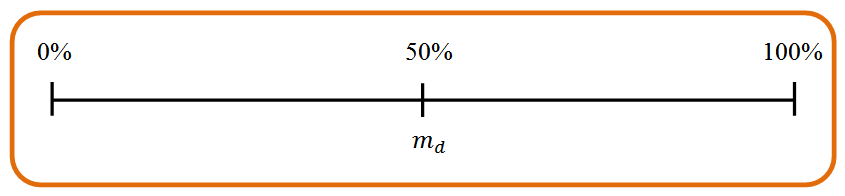
\includegraphics[trim=0 0cm 0 0cm, scale=0.65]{medpos_mediana.png}
%\setlength{\abovecaptionskip}{0.5pt}
%\caption{Taxa de ocupação hoteleira}
\label{fig:medpos_mediana} % Unique label used for referencing the figure in-text
\end{figure}


\subsection{Mediana para dados brutos}
\vspace{0,3cm}

\subsubsection{Número ímpar de dados (n ímpar)}
\vspace{0,3cm}

Quando o número de dados é ímpar existe um único elemento na posição central do conjunto de dados ordenados. Neste caso, a mediana é igual a este elemento. \\


\begin{example}

O conjunto de dados ordenados 

\begin{center}
	\begin{tabular}{c c c c c}
	\hline
	1 & 3 & 5 & 7 & 9 \\
	\hline
	\end{tabular}
\end{center}

\noindent tem mediana $m_d=5$ pois este é o elemento central deste conjunto de dados ordenados. Observe que este valor divide o conjunto de dados ordenados em duas partes iguais.

\end{example}

\vspace{0,3cm}

\subsubsection{Número par de dados (n par)}
\vspace{0,3cm}

Quando o número de dados é par existem dois elementos centrais no conjunto de dados ordenados. Neste caso, a mediana é igual a média desses dois valores. \\

\begin{example}

O conjunto de dados ordenados 

\begin{center}
	\begin{tabular}{c c c c c}
	\hline
	3 & 5 & 7 & 9 \\
	\hline
	\end{tabular}
\end{center}

\noindent tem mediana \, $m_d=6$ \, pois este valor é a média dos dois elementos centrais do conjunto de dados ordenados, ou seja, 

\begin{center}
$m_d=\frac{5+7}{2}=6$.
\end{center}

Observe que este valor divide o conjunto de dados ordenados em duas partes iguais. Note também que a mediana não precisa ser igual a nenhum dos elementos do conjunto de dados.

\end{example}

\vspace{0,3cm}

\subsubsection{Fórmula para calcular a mediana}
\vspace{0,3cm}

Pode-se, ainda, utilizar a fórmula apresentada na Equação~\ref{eq:medianadadosbrutos} para calcular a mediana.

\begin{eBox}
\vspace{-0.5cm}
\begin{equation} \label{eq:medianadadosbrutos}
 m_d =
       \begin{cases}
        	\displaystyle x_{(\frac{n+1}{2})}, & \mbox{se } n \mbox{ for ímpar;} \\
       		& \\
       		\displaystyle \frac{x_{(\frac{n}{2})}+x_{(\frac{n}{2}+1)}}{2}, & \mbox{se }  n \mbox{ for par.}
       \end{cases}
\end{equation}
\end{eBox}

\vspace{0,5cm}

\begin{example}

Considere o conjunto de dados ordenados:

\begin{center}
	\begin{tabular}{c c c c c}
	\hline
	1 & 3 & 5 & 7 & 9 \\
	\hline
	\end{tabular}
\end{center}


Como  $n=5$  é ímpar, então:

\begin{center}
$m_d= \displaystyle x_{(\frac{n+1}{2})}= x_{(\frac{5+1}{2})}= x_{(\frac{6}{2})}=x_3=5.$ 
\end{center}

\vspace{0,5cm}

\noindent Considere, agora, o conjunto de dados ordenados:

\begin{center}
	\begin{tabular}{c c c c}
	\hline
	3 & 5 & 7 & 9 \\
	\hline
	\end{tabular}
\end{center}


Como  $n=4$  é par, então:

\begin{center}
$m_d=\displaystyle \frac{x_{(\frac{n}{2})}+x_{(\frac{n}{2}+1)}}{2}=\frac{x_{(\frac{4}{2})}+x_{(\frac{4}{2}+1)}}{2}
=\frac{x_{2}+x_{3}}{2}=\frac{5+7}{2}=\frac{12}{2}=6.$
\end{center}

\end{example}

\vspace{0,3cm}

Na Lista~\ref{lst:Rmediana1} são apresentados os comandos do software R para calcular a mediana. \\

\begin{scriptsize}
	\estiloR
	\begin{lstlisting}[caption={Comandos do software R}, label=lst:Rmediana1]
	# Entrando com os dados no R (n ímpar)
	dados1 <- c(1, 3, 5, 7, 9)
	
	# Mediana
	median(dados1)
	
	# Entrando com os dados no R (n par)
	dados2 <- c(3, 5, 7, 9)
	
	# Mediana
	median(dados2)

	\end{lstlisting}
\end{scriptsize}



\subsection{Mediana para dados agrupados}
\vspace{0,3cm}
\subsubsection{Mediana para dados discretos agrupados}
\vspace{0,3cm}

Quando dados quantitativos discretos estão agrupados em uma tabela de distribuição de frequências, utiliza-se a frequência acumulada para verificar em qual classe está o elemento da posição central $x_{(\frac{n+1}{2})}$, caso $n$ for ímpar, ou os dois elementos centrais $x_{(\frac{n}{2})}$ e $x_{(\frac{n}{2}+1)}$, caso $n$ for par. A frequência acumulada de uma determinada linha é a soma das frequências das linhas anteriores com a frequência desta linha (Tabela~\ref{tab:tabfreqac}).

	\begin{table}[h]
	\caption{Obtenção das frequências acumuladas}
	\label{tab:tabfreqac} 
	\vspace{-0.1cm}
	\centering
	\begin{tabular}{c c c}
	\toprule
	\textbf{Dados} ($\bm{x_i}$) & \textbf{Frequências} ($\bm{f_i}$) & \textbf{Frequências acumuladas} ($\bm{F_{ac}}$) \\
	\midrule
	$x_1$  &  $f_1$  &  $\bm{f_1}$  \\
	$x_2$  &  $f_2$  &  $f_1+\bm{f_2}$  \\
	$x_3$  &  $f_3$  &  $f_1+f_2+\bm{f_3}$  \\
	\vdots  & \vdots &  \vdots \\
	$x_k$  &  $f_k$  &  $f_1+f_2+f_3+\hdots+\bm{f_k}$  \\
	\hline
	Total  &  $\sum{f_i}$ & $-$ \\
	\bottomrule
	\end{tabular} \\
	\end{table}

\vspace{2cm}

\begin{example}

Considere a tabela de distribuição de frequências do número de filhos de vinte funcionários, contendo as frequências acumuladas (Tabela~\ref{tab:distnumfilhosac}).


	\begin{table}[h]
	\caption{Distribuição de frequências do número de filhos de vinte funcionários}
	\label{tab:distnumfilhosac} 
	\vspace{-0.1cm}
	\centering
	\begin{tabular}{c c c}
	\toprule
	\textbf{Número de filhos} ($\bm{x_i}$) & \textbf{Frequências} ($\bm{f_i}$) & \textbf{Frequências acumuladas} ($\bm{F_{ac}}$) \\
	\midrule
	0 & 6 & 6 \\
	1 & 8 & \textcolor{ocre}{\bf 14} \\
	2 & 4 & 18 \\
	3 & 1 & 19 \\
	4 & 0 & 19 \\
	5 & 1 & 20 \\
	\hline
	Total & $\sum{f_i}=20$ & $-$\\
	\bottomrule
	\end{tabular} \\
	\end{table}
	
Como $n=20$ ($n$ par), então a mediana é a média dos dois elementos centrais: $x_{10}$ e $x_{11}$. Observando as frequências acumuladas pode-se ver que $x_{10}$ e $x_{11}$ não estão na primeira linha da tabela, pois, a frequência acumulada da primeira linha é $6$, ou seja, até a primeira linha tem apenas 6 elementos (vai até o elemento $x_6$). Como a frequência acumulada da segunda linha é $14$ então até a segunda linha tem 14 elementos (vai desde o elemento $x_7$ até o elemento $x_{14}$), ou seja, os elementos $x_{10}$  e $x_{11}$ estão ambos na segunda linha. Como na segunda linha todos os elementos são iguais ao número $1$ (isto é, $x_i=1$), então:

\begin{center}
$m_d=\displaystyle \frac{x_{10}+x_{11}}{2}=\frac{1+1}{2}=1$.
\end{center}

\end{example}

\vspace{0,3cm}

Na Lista~\ref{lst:Rmediana2} são apresentados os comandos do software R para calcular a mediana para dados discretos agrupados em uma distribuição de frequências. \\

\begin{scriptsize}
	\estiloR
	\begin{lstlisting}[caption={Comandos do software R}, label=lst:Rmediana2]
	# Entrando com os dados (xi) e as frequências (fi) no R
	xi <- c(0, 1, 2, 3, 4, 5)
	fi <- c(6, 8, 4, 1, 0, 1)

	# Desagrupando os dados no R
	dados <- rep(xi, fi); dados
	
	# Mediana
	median(dados)

	\end{lstlisting}
\end{scriptsize}


\subsubsection{Mediana para dados contínuos agrupados}
\vspace{0,3cm}

Para dados quantitativos contínuos agrupados em uma tabela de distribuição de frequências (em classes) deve-se determinar a classe mediana, que é a classe que contém o elemento da posição $n/2$ (independentemente de $n$ ser par ou ímpar). Depois, determina-se o valor da mediana utilizando a Equação~\ref{eq:medianadadoscontinuos}.

\begin{eBox}
\vspace{-0.5cm}
\begin{equation} \label{eq:medianadadoscontinuos}
	m_d=LI_{md}+\frac{\frac{n}{2}-F_{ac}^*}{f_{md}} \times c_{md}
\end{equation}
\end{eBox}

\vspace{0,3cm}
\noindent em que:
\vspace{0,3cm}

\begin{itemize}

\item $LI_{md}$ é o limite inferior da classe mediana;

\item $c_{md}$ é a amplitude da classe mediana $(c_{md}=LS_{md}-LI_{md})$;

\item $f_{md}$ é a frequência da classe mediana;

\item $F_{ac}^*$ é a frequência acumulada da {\bf classe anterior} à classe mediana. Se a classe mediana for a primeira classe então $F_{ac}^*$ será igual a zero.

\end{itemize}
	
\vspace{0,5cm}


\begin{example}

Na Tabela~\ref{tab:distdadoscontinuos} é apresentada a distribuição de frequências dos salários de 100 indivíduos (em x sal. mín.).

	\begin{table}[h]
	\caption{Distribuição de frequências dos salários de 100 indivíduos}
	\label{tab:distdadoscontinuos} 
	\vspace{-0.1cm}
	\centering
	\begin{tabular}{c c c}
	\toprule
	\textbf{Classes} & \textbf{Frequências} ($\bm{f_i}$) & \textbf{Frequências acumuladas} ($\bm{F_{ac}}$) \\
	\midrule
	$1,5 \vdash 2,0$ & 3 & 3 \\
	$2,0 \vdash 2,5$ & 16 & 19 \\
	$2,5 \vdash 3,0$ & 32 & 51 \\
	$3,0 \vdash 3,5$ & 33 & 84 \\
	$3,5 \vdash 4,0$ & 11 & 95 \\
	$4,0 \vdash 4,5$ & 4 & 99 \\
	$4,5 \vdash 5,0$ & 1 & 100 \\
	\hline
	Total & $100$ & $-$\\
	\bottomrule
	\end{tabular} \\
	\end{table}
	
	
Como $n=100$, então $n/2=100/2=50$, e dessa forma, o elemento $x_{50}$ está na terceira classe pois a frequência acumulada da terceira classe é igual a $51$ (esta classe inclui os elementos de $x_{20}$ até $x_{51}$). Então a terceira classe é a classe mediana (classe que contém a mediana). \\

Na Figura~\ref{fig:medpos_mediana2} são apresentadas as localizações na tabela dos itens necessários para o cálculo da mediana. \\

\begin{figure}[h!]
\centering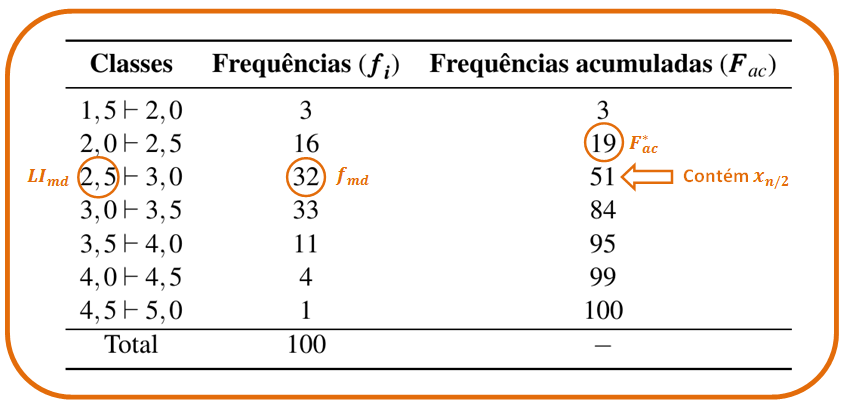
\includegraphics[trim=0 0cm 0 0cm, scale=0.65]{medpos_mediana2.png}
%\setlength{\abovecaptionskip}{0.5pt}
\caption{Itens para o cálculo da mediana}
\label{fig:medpos_mediana2} % Unique label used for referencing the figure in-text
\end{figure}

Assim, os itens necessários para efetuar o cálculo da mediana são:

\begin{itemize}
\item $n/2=100/2=50$;
\item $LI_{md}=2,5$;
\item $F_{ac}^*=19$;
\item $f_{md}=32$;
\item $c_{md}=3,0-2,5=0,5$. \\
\end{itemize}

\vspace{2cm}

Portanto, a mediana é calculada por: 

\begin{ceqn}
\begin{align*}
\centering
m_d
&= LI_{md}+\frac{\frac{n}{2}-F_{ac}}{f_{md}} \times c_{md} \\ \\
&= 2,5+\frac{50-19}{32} \times 0,5 \\ \\
&= 2,985 \mbox{ salários}. 
\end{align*}
\end{ceqn}

\end{example}

\vspace{0,3cm}

\subsubsection{Propriedades da mediana}

\begin{enumerate}

\item é única em um conjunto de dados e nem sempre tem existência real, ou seja, nem sempre é igual a um determinado valor observado;

\item não depende de todos os valores do conjunto de dados, podendo não se alterar com a modificação de alguns deles; 

\item não é influenciada por valores atípicos do conjunto de dados;

\item somando ou subtraindo uma constante não nula aos valores da variável a mediana "receberá" a soma ou subtração da constante;

\item multiplicando ou dividindo uma constante não nula aos valores da variável, a mediana ficará multiplicada ou dividida pela constante.

\end{enumerate}



%------------------------------------------------

\section{Moda}
\vspace{0,3cm}

\subsection{Moda para dados brutos}
\vspace{0,3cm}

A moda é o elemento do conjunto de dados que ocorre com maior frequência. \\

\begin{example}

Considere o conjunto de dados :

\begin{center}
	\begin{tabular}{c c c c c c c c c c c c}
	\hline
	0 & 0 & 2 & 5 & 3 & 7 & 4 & 7 & 8 & 7 & 9 & 6 \\
	\hline
	\end{tabular}
\end{center}

A moda deste conjunto de dados é o número 7  porque este é o elemento que ocorre o maior número de vezes.

\end{example}

\vspace{0,3cm}

\noindent {\bf Observação}: Um conjunto de dados pode não ter moda ou ter duas ou mais modas. \\

\begin{example}

Considere o conjunto de dados :

\begin{center}
	\begin{tabular}{c c c c c c}
	\hline
	0 & 2 & 4 & 6 & 8 & 10 \\
	\hline
	\end{tabular}
\end{center}

Este conjunto de dados não tem moda pois nenhum elemento ocorre com maior frequência. \\

Considere, agora, o conjunto de dados:

\begin{center}
	\begin{tabular}{c c c c c c c c c}
	\hline
	1 & 2 & 2 & 3 & 4 & 4 & 5 & 6 & 7 \\
	\hline
	\end{tabular}
\end{center}

Este conjunto de dados tem duas modas: 2 e 4.

\end{example}

\vspace{0,3cm}

Na Lista~\ref{lst:Rmoda1} são apresentados os comandos do software R para calcular a moda para dados brutos. \\

\begin{scriptsize}
	\estiloR
	\begin{lstlisting}[caption={Comandos do software R}, label=lst:Rmoda1]
	# Entrando com os dados no R
	dados <- c(0, 0, 2, 5, 3, 7, 4, 7, 8, 7, 9, 6)

	# Contando as frequências dos elementos
	tab <- table(dados)

	# Moda (elemento com maior frequência)
	as.numeric(names(tab)[tab==max(tab)])

	\end{lstlisting}
\end{scriptsize}



\subsection{Moda para dados agrupados}

\subsubsection{Moda para dados discretos agrupados}

Para dados quantitativos discretos agrupados em uma tabela de distribuição de frequências a moda é o elemento que tem a maior frequência (elemento que ocorre maior número de vezes). \\


\begin{example}

Considere os dados quantitativos discretos agrupados em uma distribuição de frequências (Tabela~\ref{tab:distdadosdiscretosmoda}). \\


	\begin{table}[h]
	\caption{Distribuição de frequências de dados quantitativos discretos}
	\label{tab:distdadosdiscretosmoda} 
	\vspace{-0.1cm}
	\centering
	\begin{tabular}{c c}
	\toprule
	\textbf{Dados} ($\bm{x_i}$) & \textbf{Frequências} ($\bm{f_i}$) \\
	\midrule
	0 & 2 \\
	1 & 0 \\
	2 & 1 \\
	3 & 1 \\
	4 & 1 \\
	5 & 1 \\
	6 & 1 \\
	7 & 3 \\
	8 & 1 \\
	9 & 1 \\
	\hline
	Total & $12$ \\
	\bottomrule
	\end{tabular} \\
	\end{table}
	

A moda é o número 7 pois $x_i=7$ é o valor que tem a maior frequência ($f_i=3$). Portanto, $m_o=7$.
	
\end{example}

\vspace{0,3cm}

Na Lista~\ref{lst:Rmoda1} são apresentados os comandos do software R para calcular a moda para dados discretos agrupados em uma distribuição de frequências. \\

\begin{scriptsize}
	\estiloR
	\begin{lstlisting}[caption={Comandos do software R}, label=lst:Rmoda1]
	# Entrando com os dados no R
	xi <- c(0, 1, 2, 3, 4, 5, 6, 7, 8, 9)
	fi <- c(2, 0, 1, 1, 1, 1, 1, 3, 1, 1)

	# Moda (elemento com maior frequência)
	xi[fi==max(fi)]

	\end{lstlisting}
\end{scriptsize}



\subsubsection{Moda para dados contínuos agrupados}
\vspace{0,3cm}

Para dados quantitativos contínuos a moda é o valor de maior densidade, ou seja, é o valor sob o qual a variável atinge o ponto mais alto de sua distribuição. \\

Para dados contínuosagrupados em uma tabela de distribuição de frequências (em classes), a classe modal (classe que contém a moda) é a classe com a maior frequência. Para determinar o valor da moda utiliza-se a Equação~\ref{eq:modadadoscontinuos} (fórmula de Czuber). \\


\begin{eBox}
\vspace{-0.5cm}
\begin{equation} \label{eq:modadadoscontinuos}
	m_o= \displaystyle LI_{mo}+\frac{\Delta_1}{\Delta_1+\Delta_2} \times c_{mo}
\end{equation}
\end{eBox}

\vspace{0,3cm}
\noindent em que:
\vspace{0,3cm}

\begin{itemize}
\item $LI_{mo}$ é o limite inferior da classe modal;
\item $c_{mo}$ é a amplitude da classe modal;
\item $\Delta_1$ é a diferença entre a frequência da classe modal e a frequência da classe imediatamente anterior;
\item $\Delta_2$ é a diferença entre a frequência da classe modal e a frequência da classe imediatamente posterior.
\end{itemize}

\vspace{0,5cm}

\begin{example}

Na Tabela~\ref{tab:distdadoscontinuos2} é apresentada a distribuição de frequências dos salários de 100 indivíduos (em x sal. mín.). \\

\begin{table}[h]
	\caption{Distribuição de frequências dos salários de 100 indivíduos}
	\label{tab:distdadoscontinuos2} 
	\vspace{-0.1cm}
	\centering
	\begin{tabular}{c c}
	\toprule
	\textbf{Classes} & \textbf{Frequências} ($\bm{f_i}$) \\
	\midrule
	$1,5 \vdash 2,0$ & 3 \\
	$2,0 \vdash 2,5$ & 16 \\
	$2,5 \vdash 3,0$ & 32 \\
	$3,0 \vdash 3,5$ & 33 \\
	$3,5 \vdash 4,0$ & 11 \\
	$4,0 \vdash 4,5$ & 4 \\
	$4,5 \vdash 5,0$ & 1 \\
	\hline
	Total & $100$ \\
	\bottomrule
	\end{tabular} \\
\end{table}


\vspace {2cm}
	
Observe que a classe com maior frequência é a quarta classe (frequência igual a 33). Portanto a quarta classe é a classe modal. \\



Os itens necessários para efetuar o cálculo da moda são:

\begin{itemize}
\item $LI_{mo}=3,0$;
\item $\Delta_1=33-32=1$;
\item $\Delta_2=33-11=22$;
\item $c_{mo}=3,5-3,0=0,5$. \\
\end{itemize}

Na Figura~\ref{fig:medpos_moda1} são apresentadas as localizações na tabela dos itens necessários para o cálculo da moda.

\begin{figure}[h]
\centering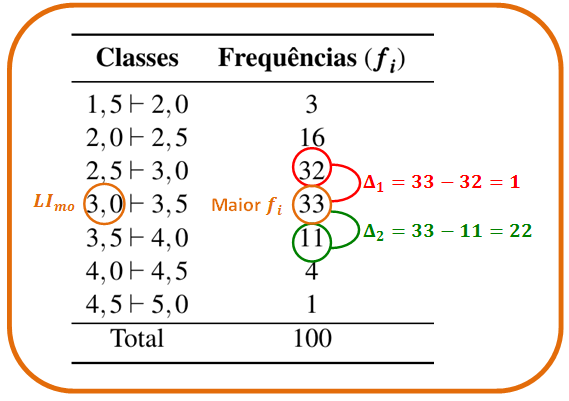
\includegraphics[trim=0 0cm 0 0cm, scale=0.65]{medpos_moda1.png}
%\setlength{\abovecaptionskip}{0.5pt}
\caption{Itens para o cálculo da moda}
\label{fig:medpos_moda1} % Unique label used for referencing the figure in-text
\end{figure}

Portanto, a moda é calculada por: 

\begin{ceqn}
\begin{align*}
\centering
m_o
&= LI_{mo}+\frac{\Delta_1}{\Delta_1+\Delta_2} \times c_{mo} \\ \\
&= 3,0+\frac{1}{1+22} \times 0,5 \\ \\
&= 3,022 \mbox{ salários}. 
\end{align*}
\end{ceqn}

\end{example}

\vspace{0,3cm}



\subsection{Moda para dados qualitativos}

A moda é a única medida de posição que também pode ser usada para descrever dados qualitativos. Nesse caso, a moda é a categoria da variável que ocorre com maior frequência. \\


\begin{example}

Na Tabela~\ref{tab:distdadosqualimoda} é apresentada a distribuição de frequências do tipo sanguíneo de 1.167 indivíduos. 

\begin{table}[h]
	\caption{Distribuição de frequências do tipo sanguíneo de 1.167 indivíduos}
	\label{tab:distdadosqualimoda} 
	\vspace{-0.1cm}
	\centering
	\begin{tabular}{c c}
	\toprule
	\textbf{Grupo sanguíneo} & \textbf{Frequências} ($\bm{f_i}$) \\
	\midrule
	O & 550 \\
	A & 456 \\
	B & 132 \\
	AB & 29 \\
	\hline
	Total & $1167$ \\
	\bottomrule
	\end{tabular} \\
\end{table}

A moda é o grupo sanguíneo O pois esta foi a categoria que ocorreu com maior frequência ($f_i=550$).


\end{example}

\subsubsection{Propriedades da moda}

\begin{itemize}
\item sempre é representada por um dos valores da variável;

\item não depende de todos os valores do conjunto de dados, podendo não se alterar com a modificação de alguns deles; 

\item não é influenciada pelos valores atípicos do conjunto de dados;

\item somando ou subtraindo uma constante não nula aos valores da variável, a moda aritmética "receberá" a soma ou subtração da constante;

\item multiplicando ou dividindo uma constante não nula aos valores da variável, a moda ficará multiplicada ou dividida pela constante.

\end{itemize}



%------------------------------------------------
\section{Utilização das medidas de tendência central}

Costa (2012) propõe os seguintes critérios para escolher entre as medidas de posição: \\

\noindent Escolha da média:
\begin{enumerate}
\item quando a distribuição dos dados é pelo menos aproximadamente simétrica;
\item quando for necessário obter posteriormente outros parâmetros que podem depender da média, como por exemplo a variância, o desvio padrão, etc.\\
\end{enumerate}

\noindent Escolha da mediana:
\begin{enumerate}
\item quando há valores extremos;
\item quando deseja-se conhecer o ponto central da distribuição;
\item quando a distribuição dos dados é muito assimétrica.\\
\end{enumerate}

\noindent Escolha da moda:
\begin{enumerate}
\item quando a medida de interesse é o ponto mais típico ou popular dos dados;
\item quando precisa-se apenas de uma rápida idéia sobre a tendência central dos dados. \\
\end{enumerate}


%------------------------------------------------

\section{Medidas separatrizes (quantis)}

Foi visto que a mediana é um valor divide o conjunto de dados ao meio, ou seja, a mediana deixa 50\% dos dados abaixo dela e 50\% acima. De um modo geral podemos definir uma medida chamada quantil de ordem $q(p)$, em que $p$ é uma proporção qualquer, $0<p<1$, tal que $100p\%$ das observações sejam menores do que $q(p)$. \\

\begin{example}

A seguir são apresentados alguns quantis e seus nomes particulares: \\

\begin{itemize}

\item $q(0,25)$: 25° percentil $\Rightarrow$ 25\% das observações são menores do que $q(0,25)$. O 25° percentil também é conhecido como 1º quartil;

\item $q(0,50)$: 50° percentil $\Rightarrow$ 50\% das observações são menores do que $q(0,50)$. Note que o 50° percentil é igual a mediana, ou seja, $q(0,50)=m_d$. A mediana também é conhecida como 2º quartil;

\item $q(0,90)$: 90° percentil $\Rightarrow$ 90\% das observações são menores do que $q(0,90)$. O 90° percentil também é conhecido como 9º decil.

\end{itemize}
		

\end{example}

\vspace{0,3cm}


\subsection{Quartis para dados brutos}

Os quartis ($q_1$, $q_2$ e $q_3$) são valores que dividem o conjunto de dados em quatro partes iguais:


\begin{figure}[h!]
\centering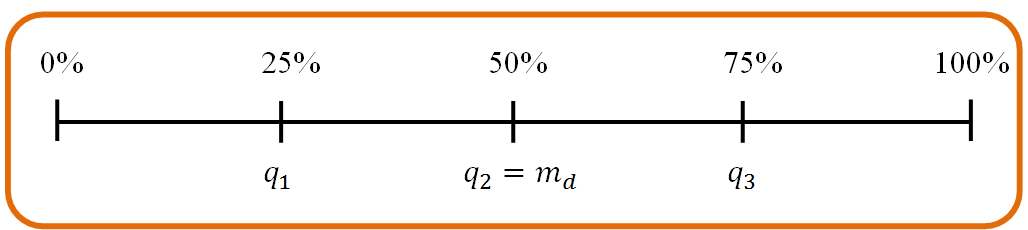
\includegraphics[trim=0 0cm 0 0cm, scale=0.53]{medpos_quartis.png}
%\setlength{\abovecaptionskip}{0.5pt}
%\caption{Taxa de ocupação hoteleira}
\label{fig:medpos_quartis} % Unique label used for referencing the figure in-text
\end{figure}

\vspace{0,3cm}

O primeiro quartil ($q_1$) é um valor tal que 25\% dos dados são menores ou iguais a ele (então os outros 75\% dos dados são maiores ou iguais a ele), o segundo quartil ($q_2$), que é igual à mediana ($m_d$), é um valor tal que 50\% dos dados são menores ou iguais a ele (então os outros 50\% dos dados são maiores ou iguais a ele) e o terceiro quartil ($q_3$) é um valor tal que 75\% dos dados são menores ou iguais a ele (então os outros 25\% dos dados são maiores ou iguais a ele). 

Para calcular os quartis primeiro deve-se ordenar o conjunto de dados. \\


\subsubsection{Obtendo os quartis de um conjunto com um número ímpar de dados}
\vspace{0,3cm}

\begin{example} \label{exemp:quartis1}

Considere o conjunto de dados:

\begin{center}
	\begin{tabular}{c c c c c c c c c}
	\hline
	3 & 4 & 1 & 5 & 7 & 9 & 2 & 10 & 6 \\
	\hline
	\end{tabular}
\end{center}

Primeiramente deve-se ordenar o conjunto de dados:

\begin{center}
	\begin{tabular}{c c c c c c c c c}
	\hline
	1 & 2 & 3 & 4 & 5 & 6 & 7 & 9 & 10 \\
	\hline
	\end{tabular}
\end{center}

Observe que $n=9$ ($n$ ímpar). Então, a mediana é o valor central dos dados ordenados, ou seja, $m_d=5$:

\begin{center}
	\begin{tabular}{c c c c c c c c c}
	\hline
	1 & 2 & 3 & 4 & \textcolor{ocre}{\bf 5} & 6 & 7 & 9 & 10 \\
	\hline
	\end{tabular}
\end{center}

Como $q_2=m_d$ então o segundo quartil já foi obtido, ou seja, $q_2=5$. \\

Para obter o primeiro quartil ($q_1$) e o terceiro quartil ($q_3$) separe o conjunto de dados ordenados em dois subconjuntos: \\

\begin{enumerate}[label=\alph*)]
\item dados ordenados à esquerda da mediana, {\bf incluindo a mediana};
\item dados ordenados à direita da mediana, {\bf incluindo a mediana}, \\
\end{enumerate}

\noindent e obtenha as medianas destes subconjuntos. Estas medianas serão, respectivamente, $q_1$ e $q_3$. \\

Assim, para o subconjunto (a):

\begin{center}
	\begin{tabular}{c c c c c}
	\hline
	1 & 2 & \textcolor{ocre}{\bf 3} & 4 & 5 \\
	\hline
	\end{tabular}
\end{center}

\noindent a mediana é igual a $3$ e, portanto, $q_1=3$. \\

Para o subconjunto (b):

\begin{center}
	\begin{tabular}{c c c c c}
	\hline
	5 & 6 & \textcolor{ocre}{\bf 7} & 9 & 10 \\
	\hline
	\end{tabular}
\end{center}

\noindent a mediana é igual a $7$ e, portanto, $q_3=7$. \\


Portanto, os quartis são: \, $q_1=3$, \, $q_2=5$ \, e \, $q_3=7$. 

\begin{center}
	\begin{tabular}{c c c c c c c c c}
	\hline
	1 & 2 & \textcolor{ocre}{\bf 3} & 4 & \textcolor{ocre}{\bf 5} & 6 & 7 & \textcolor{ocre}{\bf 9} & 10 \\
	\hline
	\end{tabular}
\end{center}

\end{example}

\noindent {\bf Observação}: Note no Exemplo~\ref{exemp:quartis1} que no conjunto de dados ordenados dois valores são menores do que $q_1$ e seis valores são maiores do que $q_1$, quatro valores são maiores do que $q_2$ e quatro valores são maiores do que $q_2$ e, por fim, seis valores são menores do que $q_3$ e dois valores são maiores do que $q_3$. Portanto os quartis dividiram o conjunto de dados em quatro partes aproximadamente iguais. \\

Na Lista~\ref{lst:Rquartis1} são apresentados os comandos do software R para calcular os quartis para um conjunto com um número ímpar de dados. \\

\begin{scriptsize}
	\estiloR
	\begin{lstlisting}[caption={Comandos do software R}, label=lst:Rquartis1]
	# Entrando com os dados no R
	dados <- c(3, 4, 1, 5, 7, 9, 2, 10, 6)
	
	# Número de elementos do conjunto de dados
	length(dados)

	# Quartis (para n ímpar)
	quantile(dados)

	# Quartis e outras medidas (mínimo, máximo e média)
	summary(dados)

	\end{lstlisting}
\end{scriptsize}


\subsubsection{Obtendo os quartis de um conjunto com um número par de dados}
\vspace{0,3cm}

\begin{example} \label{exemp:quartisnpar}

Considere o conjunto de dados:

\begin{center}
	\begin{tabular}{c c c c c c c c c c}
	\hline
	11 & 3 & 4 & 1 & 5 & 7 & 9 & 2 & 10 & 6 \\
	\hline
	\end{tabular}
\end{center}

Primeiramente deve-se ordenar o conjunto de dados:

\begin{center}
	\begin{tabular}{c c c c c c c c c c}
	\hline
	1 & 2 & 3 & 4 & \textcolor{ocre}{\bf 5} & \textcolor{ocre}{\bf 6} & 7 & 9 & 10 & 11 \\
	\hline
	\end{tabular}
\end{center}

Observe que $n=10$ ($n$ par).  Então, a mediana é a média dos dois valores centrais dos dados ordenados, ou seja, 
\begin{center}
$\displaystyle m_d=\frac{5+6}{2}=5,5.$
\end{center}

Como $q_2=m_d$ então o segundo quartil já foi obtido, ou seja, $q_2=5,5$. Observe que, neste caso, a mediana não é um valor pertencente ao conjunto de dados.\\

Para obter o primeiro quartil ($q_1$) e o terceiro quartil ($q_3$) separe o conjunto de dados ordenados em dois subconjuntos: \\

\begin{enumerate}[label=\alph*)]
\item dados ordenados à esquerda da mediana, {\bf sem incluir a mediana};
\item dados ordenados à direita da mediana, {\bf sem incluir a mediana}, \\
\end{enumerate}

\noindent e obtenha as medianas destes subconjuntos. Estas medianas serão, respectivamente, $q_1$ e $q_3$. \\

Assim, para o subconjunto (a):

\begin{center}
	\begin{tabular}{c c c c c}
	\hline
	1 & 2 & \textcolor{ocre}{\bf 3} & 4 & 5 \\
	\hline
	\end{tabular}
\end{center}

\noindent a mediana é igual a $3$ e, portanto, $q_1=3$. \\

Para o subconjunto (b):

\begin{center}
	\begin{tabular}{c c c c c}
	\hline
	6 & 7 & \textcolor{ocre}{\bf 9} & 10 & 11 \\
	\hline
	\end{tabular}
\end{center}

\noindent a mediana é igual a $9$ e, portanto, $q_3=9$. \\


Portanto, os quartis são: \, $q_1=3$, \, $q_2=5,5$ \, e \, $q_3=9$. 


\end{example}

\vspace{0,3cm}

\noindent {\bf Observação}: As formas de se calcular os quartis não são as únicas, existem várias formas diferentes de se calcular quartis. Na Lista~\ref{lst:Rquartis2} são apresentados os comandos do software R para calcular os quartis para um conjunto com um número par de dados, como foi visto no Exemplo~\ref{exemp:quartisnpar}, e também por outros métodos que não foram abordados neste material (os resultados são diferentes). \\

\begin{scriptsize}
	\estiloR
	\begin{lstlisting}[caption={Comandos do software R}, label=lst:Rquartis2]
	# Entrando com os dados no R
	dados <- c(11, 3, 4, 1, 5, 7, 9, 2, 10, 6)
	
	# Número de elementos do conjunto de dados
	length(dados)

	# Quartis (para n par, método abordado no material)
	quantile(dados, type=5)

	# Quartis (método diferente do abordado no material)
	quantile(dados)

	# Quartis e outras medidas (método diferente do abordado no material)
	summary(dados)

	\end{lstlisting}
\end{scriptsize}

\noindent {\bf Observação}: Na Lista~\ref{lst:Rquartis2} o argumento  \texttt{type=5} do comando \texttt{quantile()} é que seleciona o método de cálculo dos quartis, para $n$ par, igual ao que foi usado neste material. \\


\subsection{Quartis para dados agrupados}
\vspace{0,3cm}

Foi visto anteriormente que a mediana para dados contínuos agrupados em classes era calculada pela Equação~\ref{eq:medianadadoscontinuos}, ou seja,

\begin{center}
$\displaystyle m_d=LI_{md}+\frac{\frac{n}{2}-F_{ac}^*}{f_{md}} \times c_{md}$.
\end{center}
	

Como a mediana é o segundo quartil ($m_d=q_2$), então, de maneira análoga são obtidas as fórmulas para o 1º quartil e para o 3º quartil, apresentadas a seguir. \\


\subsubsection{Determinação do 1º quartil}
\vspace{0,3cm}

\begin{enumerate}

\item calcule $n/4$;
\item identifique a classe $q_1$ pela frequência acumulada. A classe $q_1$ é a classe que contém o elemento da posição $n/4$;
\item aplique a Equação~\ref{eq:q1dadoscontinuos} para obter o 1º quartil:

\begin{eBox}
\vspace{-0.5cm}
\begin{equation} \label{eq:q1dadoscontinuos}
	q_1=LI_{q_1}+\frac{\frac{n}{4}-F_{ac}^*}{f_{q_1}} \times c_{q_1}
\end{equation}
\end{eBox}

\end{enumerate}

\noindent em que:

\begin{itemize}
\item $LI_{q_1}$ é o limite inferior da classe do 1º quartil;
\item $c_{q_1}$ é a amplitude da classe do 1º quartil;
\item $f_{q_1}$ é a frequência da classe do 1º quartil;
\item $F_{ac}^*$ é a frequência acumulada da {\bf classe anterior} à classe do 1º quartil. Se a classe do 1º quartil for a primeira classe então $F_{ac}^*$ será igual a zero. \\
\end{itemize}



\subsubsection{Determinação do 3º quartil}
\vspace{0,3cm}

\begin{enumerate}

\item calcule $3n/4$;
\item identifique a classe $q_3$ pela frequência acumulada. A classe $q_3$ é a classe que contém o elemento da posição $3n/4$;
\item aplique a Equação~\ref{eq:q3dadoscontinuos} para obter o 3º quartil:

\begin{eBox}
\vspace{-0.5cm}
\begin{equation} \label{eq:q3dadoscontinuos}
	q_3=LI_{q_3}+\frac{\frac{3n}{4}-F_{ac}^*}{f_{q_3}} \times c_{q_3}
\end{equation}
\end{eBox}

\end{enumerate}

\noindent em que:

\begin{itemize}
\item $LI_{q_3}$ é o limite inferior da classe do 3º quartil;
\item $c_{q_3}$ é a amplitude da classe do 3º quartil;
\item $f_{q_3}$ é a frequência da classe do 3º quartil;
\item $F_{ac}^*$ é a frequência acumulada da {\bf classe anterior} à classe do 3º quartil. Se a classe do 3º quartil for a primeira classe então $F_{ac}^*$ será igual a zero. \\
\end{itemize}


\begin{example}\label{exemp:distpesoscriancas}

Considere a distribuição de frequências dos pesos, em kg, de 56 crianças e adolescentes apresentada na Tabel~\ref{tab:distpesoscriancas}. \\

\begin{table}[h]
	\caption{Distribuição de frequências dos pesos, em kg, de 56 crianças e adolescentes}
	\label{tab:distpesoscriancas} 
	\vspace{-0.1cm}
	\centering
	\begin{tabular}{l c c l}
	\toprule
	\textbf{Pesos (kg)} & \textbf{Frequências} ($\bm{f_i}$) & \textbf{Frequências acumuladas} ($\bm{F_{ac}}$) \\
	\midrule
	\, $7 \vdash 17$  &  6  &  6  \\
	\textcolor{ocre}{$ \bm{17 \vdash 27}$}  &  \textcolor{ocre}{\bf 15}  &  \textcolor{ocre}{\bf 21}  & \textcolor{ocre}{$\bm{\Leftarrow}$ \,\, {\bf classe} $\bm{q_1}$} \\
	
	\textcolor{verdescuro}{$\bm{27 \vdash 37$}}  &  \textcolor{verdescuro}{{\bf 20}}  &  \textcolor{verdescuro}{{\bf 41}}  & \textcolor{verdescuro}{$\bm{\Leftarrow}$ \,\, {\bf classe} $\bm{q_2}$}  \\
	
	\textcolor{ocre}{$\bm{37 \vdash 47}$}  &  \textcolor{ocre}{{\bf 10}}  &  \textcolor{ocre}{{\bf 51}}  & \textcolor{ocre}{$\bm{\Leftarrow}$ \,\, {\bf classe} $\bm{q_3}$}  \\
	$47 \vdash 57$  &  5  &  56  \\
	\hline
	Total & $56$ & $-$ \\
	\bottomrule
	\end{tabular} \\
\end{table}


Observando as frequências acumuladas são obtidas as classes que contém os quartis (classe $q_1$, classe $q_2$ e classe $q_3$): \\

\begin{itemize}

\item $\displaystyle \frac{n}{4}=\frac{56}{4}=14 \,\, \Rightarrow$ \, a 2ª classe ($F_{ac}=21$ $\Rightarrow$ elementos: $x_7$ até $x_{21}$) contém o elemento da posição $n/4=14$. Portanto esta é a classe $q_1$; \\

\item $\displaystyle \frac{n}{2}=\frac{56}{2}=28 \,\, \Rightarrow$ \, a 3ª classe ($F_{ac}=41$ $\Rightarrow$ elementos: $x_{22}$ até $x_{41}$) contém o elemento da posição $n/2=28$. Portanto esta é a classe $q_2$; \\

\item $\displaystyle \frac{3 \times n}{4}=\frac{3 \times 56}{4}=42 \,\, \Rightarrow$ \, a 4ª classe ($F_{ac}=51$ $\Rightarrow$ elementos: $x_{42}$ até $x_{51}$) contém o elemento da posição $3n/4=42$. Portanto esta é a classe $q_3$. \\

\end{itemize}


Após encontrar as classes deve-se obter os itens das fórmulas (Equações~\ref{eq:q1dadoscontinuos}, \ref{eq:medianadadoscontinuos} e \ref{eq:q3dadoscontinuos}): \\

\begin{itemize}
\item 	Itens para calcular $q_1$:\, $LI_{q_1}=17$,\,   $n/4=14$,\,   $F_{ac}^*=6$,\,  $f_{q_1}=15$,\,  $c_{q_1}=10$; \\
\item 	Itens para calcular $q_2=m_d$:\, $LI_{m_d}=27$,\,   $n/2=28$,\,   $F_{ac}^*=21$,\,  $f_{m_d}=20$,\,  $c_{m_d}=10$; \\
\item 	Itens para calcular $q_3$:\, $LI_{q_3}=37$,\,   $3n/4=42$,\,   $F_{ac}^*=41$,\,  $f_{q_3}=10$,\,  $c_{q_3}=10$. \\
\end{itemize}

Após obter os itens das fórmulas basta substituí-los nas respectivas equações para calcular os quartis: \\

\vspace{4cm}

\noindent {\bf 1º quartil:}

\begin{ceqn}
\begin{align*}
\centering
q_1
&= \displaystyle LI_{q_1}+\frac{\frac{n}{4}-F_{ac}^*}{f_{q_1}} \times c_{q_1} \\ \\
&= \displaystyle 17+\frac{14-6}{15} \times 10 \\ \\
&= 22,3 \,\, kg\\ \\
\end{align*}
\end{ceqn}


\noindent {\bf 2º quartil:}

\begin{ceqn}
\begin{align*}
\centering
q_2=m_d
&= \displaystyle LI_{m_d}+\frac{\frac{n}{2}-F_{ac}^*}{f_{m_d}} \times c_{m_d} \\ \\
&= \displaystyle 27+\frac{28-21}{20} \times 10 \\ \\
&= 30,5 \,\, kg\\ \\
\end{align*}
\end{ceqn}

\noindent {\bf 3º quartil:}

\begin{ceqn}
\begin{align*}
\centering
q_3
&= \displaystyle LI_{q_3}+\frac{\frac{3 \times n}{4}-F_{ac}^*}{f_{q_3}} \times c_{q_3} \\ \\
&= \displaystyle 37+\frac{42-41}{10} \times 10 \\ \\
&= 38,0 \,\, kg\\ \\
\end{align*}
\end{ceqn}



\end{example}

\subsection{Percentis}

Dependendo do quantil desejado, por exemplo, o 22º percentil ($P_{22}$), pode haver dificuldades em calculá-lo para dados brutos. Sendo assim, pode-se calcular os percentis utilizando dados agrupados.\\

O percentil de ordem $i$, em que $i$ é um número de 1 a 100, pode ser calculado pela Equação~\ref{eq:pqdadoscontinuos}. \\

\begin{eBox}
\vspace{-0.5cm}
\begin{equation} \label{eq:pqdadoscontinuos}
	P_i=\displaystyle LI_{P_i}+\frac{\frac{i \times n}{100}-F_{ac}^*}{f_{P_i}} \times c_{P_i}
\end{equation}
\end{eBox}

\noindent em que: \\

\begin{itemize}
\item $LI_{P_i}$ é o limite inferior da classe $P_i$;
\item $n$ é o tamanho da amostra;
\item $F_{ac}^*$ é a frequência acumulada da {\bf classe anterior} à classe $P_i$;
\item $f_{P_i}$ é a frequência da classe $P_i$;
\item $c_{P_i}$ é a amplitude da classe $P_i$. \\

\end{itemize}

\noindent {\bf Observação}: A classe $P_i$ é a classe que contém o elemento da posição $\frac{i \times n}{100}$. Para localizar esta classe deve-se utilizar as frequências acumuladas. \\

\begin{exercise}
Utilizando a distribuição de frequências dos pesos de crianças e adolescentes (Tabela~\ref{tab:distpesoscriancas}), apresentada no Exemplo~\ref{exemp:distpesoscriancas}, determine e interprete o 90º percentil ($P_{90}$). 

\end{exercise}


%------------------------------------------------

\section{Boxplot}

As medidas que foram abordadas em seções anteriores: mínimo, máximo e quartis, permitem traçar o {\itshape Boxplot} (ou diagrama de caixa) que ajuda a entender a informação contida em um conjunto de dados.

O Boxplot dá uma idéia da posição, dispersão, assimetria, caudas e dados discrepantes. A posição central é dada pela mediana e a dispersão é dada pela distância interquartílica. As posições relativas de $q_1$, $q_2$ e $q_3$ no Boxplot também dão uma noção da assimetria (será visto no capítulo~\ref{cap:assimetriaecurtose}) da distribuição da variável. \\

Na Figura~\ref{fig:boxplot1} são apresentados os elementos de um Boxplot e também uma visão geral da aparência deste tipo de gráfico. 

\begin{figure}[h!]
\centering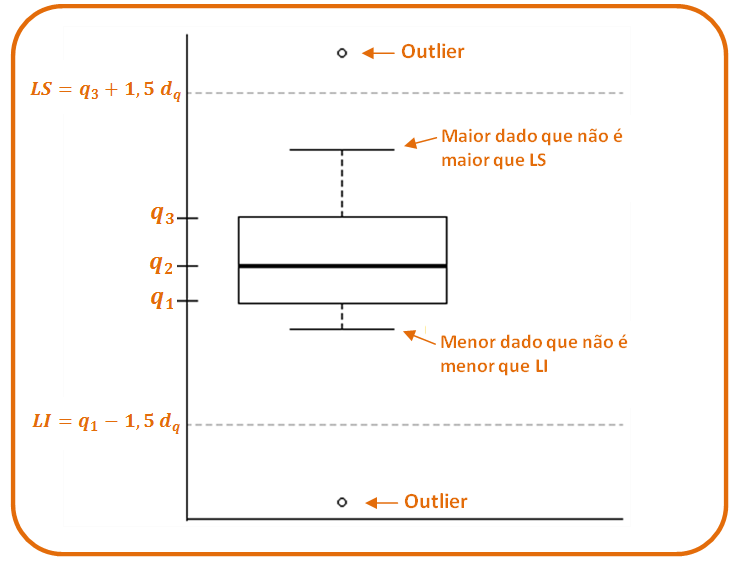
\includegraphics[trim=0 0cm 0 0cm, scale=0.7]{boxplot1.png}
%\setlength{\abovecaptionskip}{0.5pt}
\caption{Elementos do Boxplot}
\label{fig:boxplot1} % Unique label used for referencing the figure in-text
\end{figure}


\subsubsection{Passos para construir o Boxplot}
\vspace{0,3cm}

\begin{enumerate}
\item desenhe um segmento de reta na posição vertical, para representar a amplitude dos dados;

\item marque nesse segmento, o primeiro, o segundo e o terceiro quartis, obedecendo a escala;

\item desenhe um retângulo de maneira que o lado inferior e o lado superior passem exatamente nas alturas dos pontos que marcam o primeiro e o terceiro quartis;

\item faça um traço diagonal dentro do retângulo na altura do ponto que marca a mediana;

\item calcule um limite inferior ($LI$) e um limite superior ($LS$) da seguinte maneira:
\begin{center}
$LI=q_1-1,5 \times d_q$ \,\,\, e  \,\,\,  $LS=q_3+1,5 \times d_q$
\end{center}

\noindent em que \, $d_q=q_3-q_1$ \, é  a distância interquartílica;
	
\item a partir do retângulo, para cima, segue uma linha até o maior valor dos dados que não seja maior que $LS$;

\item a partir do retângulo, para baixo, segue uma linha até o menor valor dos dados que não seja menor que $LI$;

\item as observações (dados) que forem maiores ou iguais ao limite superior ou menores ou iguais ao limite inferior são valores atípicos, também chamados de {\itshape outliers}, e são representados no gráfico por "bolinhas". \\
\end{enumerate}


\begin{example}

Considere o conjunto de dados ordenados:

\begin{center}
	\begin{tabular}{c c c c c c c c c c}
	\hline
	1 & 2 & \textcolor{ocre}{\bf 3} & 4 & \textcolor{ocre}{\bf 5} & 6 & \textcolor{ocre}{\bf 7} & 10 & 16 \\
	\hline
	\end{tabular}
\end{center}

Os quartis deste conjunto de dados são:

\begin{itemize}
\item $q_1=3$;
\item $q_2=m_d=5$;
\item $q_3=7$. \\
\end{itemize}

Outros elementos necessários para construir o Boxplot:

\begin{itemize}
\item $d_q=q_3-q_1=7-3=4$;
\item $LI=q_1-1,5 \times d_q=3-1,5 \times 4=-3$;
\item $LS=q_3+1,5 \times d_q=7+1,5 \times 4=13$;
\item menor valor do conjunto de dados que não é menor do que $LI: \, x=1$;
\item maior valor do conjunto de dados que não é maior do que $LS: \, x=10$;
\item {\itshape outliers} (valores menores do que $LI$ ou maiores do que $LS$): $x=16$. \\
\end{itemize}

Utilizando os quartis e os demais elementos apresentados acima pode-se construir o Boxplot (Figura~\ref{fig:boxplot2}).

\end{example}

\vspace{0,5cm}

Na Lista~\ref{lst:Rboxplot1} são apresentados os comandos do software R para gerar o Boxplot. \\

\begin{scriptsize}
	\estiloR
	\begin{lstlisting}[caption={Comandos do software R}, label=lst:Rboxplot1]
	# Entrando com os dados no R
	dados <- c(1, 2, 3, 4, 5, 6, 7, 10, 16)

	# Gerando o Boxplot
	boxplot(dados, ylab="Nome da variável")
	
	# Alterando os valores do eixo y do Boxplot
	boxplot(dados, ylab="Nome da variável",axes=F, ylim=c(0,17))
	axis(2,c(1,3,5,7,10,16))
	box()

	\end{lstlisting}
\end{scriptsize}

\begin{figure}[h!]
\centering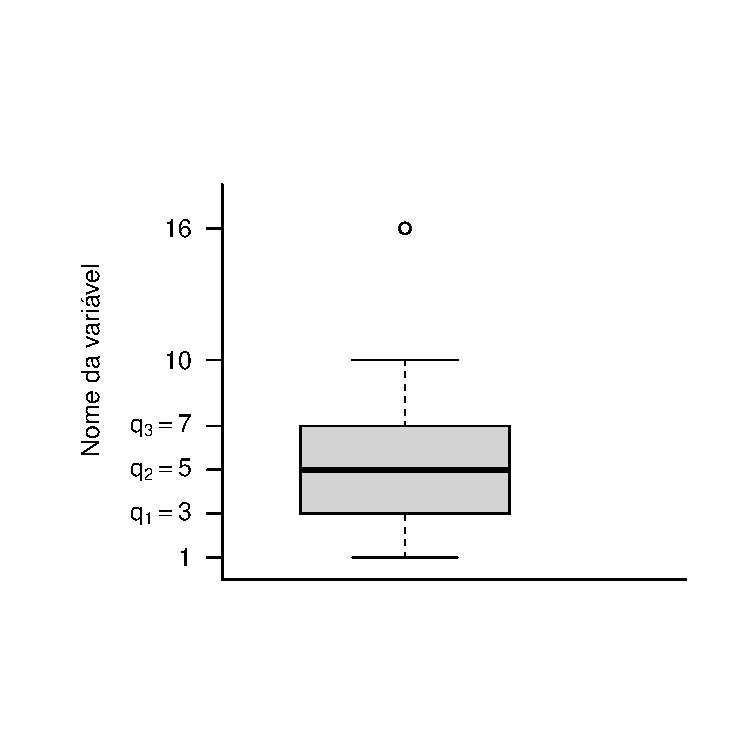
\includegraphics[trim=0cm 2cm 0cm 2.5cm, scale=0.8]{boxplot2.pdf}
\setlength{\abovecaptionskip}{0.5pt}
\caption{Boxplot}
\label{fig:boxplot2} % Unique label used for referencing the figure in-text
\end{figure}


\subsection{Boxplot comparativo}

Outra utilidade do Boxplot é na comparação de diferentes conjuntos de dados. \\

\begin{example}\label{exemp:boxplotcomp}

Foi feito um experimento para comparar dois métodos de treinamento para a execução de um serviço especializado. Vinte homens foram selecionados para esse treinamento. Dez foram escolhidos ao acaso e treinados pelo método A. Outros dez foram treinados pelo método B. Concluído o período de treinamento, todos os homens executaram o serviço e foi medido o tempo de cada um. Os dados são apresentados na Tabela~\ref{tab:boxplotcomp}.

\begin{table}[h]
	\caption{Tempo (em minutos) para execução do serviço, segundo o método de treinamento}
	\label{tab:boxplotcomp} 
	\vspace{-0.1cm}
	\centering
	\begin{tabular}{c c}
	\toprule
	\textbf{Método A} & \textbf{Método B} \\
	\midrule
	11 & 23 \\
	20 & 46 \\
	5 & 13 \\
	23 & 19 \\
	16 & 23 \\
	21 & 17 \\
	18 & 28 \\
	16 & 36 \\
	27 & 25 \\
	24 & 28 \\
	\bottomrule
	\end{tabular} \\
\end{table}

A comparação do tempo de execução de serviço pelos métodos A e B pode ser feita utilizando um Boxplot comparativo que consiste em dois Boxplots em um mesmo sistema de eixos cartesianos. O Boxplot comparativo dos métodos de treinamento é apresentado na Figura~\ref{fig:boxplot3}.


\begin{figure}[H]
\centering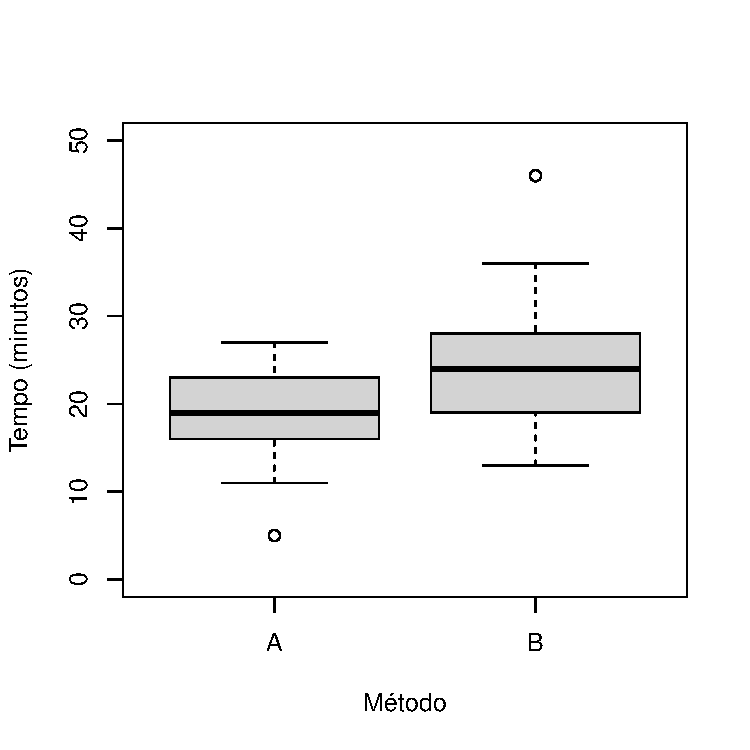
\includegraphics[trim=0cm 0.5cm 0cm 2cm, scale=0.8]{boxplot3.pdf}
%\setlength{\abovecaptionskip}{0.5pt}
\caption{Boxplot comparativo dos métodos de treinamento}
\label{fig:boxplot3} % Unique label used for referencing the figure in-text
\end{figure}

Observe pela Figura~\ref{fig:boxplot3} que os homens que foram treinados pelo método A parecem estar executando o serviço em um tempo menor do que os que foram treinados pelo método B.

\end{example} 

\vspace{0,3cm}

Na Lista~\ref{lst:Rboxplot2} são apresentados os comandos do software R para gerar um Boxplot comparativo. \\

\begin{scriptsize}
	\estiloR
	\begin{lstlisting}[caption={Comandos do software R}, label=lst:Rboxplot2]
	# Entrando com os dados no R
	A <- c(11, 20, 5, 23, 16, 21, 18, 16, 27, 24)
	B <- c(23, 46, 13, 19, 23, 17, 28, 36, 25, 28)

	# Gerando o Boxplot comparativo
	boxplot(A,B,names=c("A","B"),xlab="Método",ylab="Tempo (minutos)")
	
	# Alterando os valores do eixo y do Boxplot
	boxplot(A,B,xlab="Método",ylab="Tempo (minutos)",axes=F,ylim=c(0,50))
	axis(1,at=c(1,2),labels=c("A","B"))
	axis(2,c(0,10,20,30,40,50))
	box()

	\end{lstlisting}
\end{scriptsize}

\vspace{0,3cm}

\noindent {\bf Observação}: Considerando ainda os dados do Exemplo~\ref{exemp:boxplotcomp}, outra forma de entrada de dados no R para fazer um Boxplot comparativo é usando a mesma estrutura da Tabela~\ref{tab:boxplotcomp2}. \\

Na Lista~\ref{lst:Rboxplot3} são apresentados os comandos do software R para gerar um Boxplot comparativo com dados na mesma estrutura da Tabela~\ref{tab:boxplotcomp2}. \\

\begin{scriptsize}
	\estiloR
	\begin{lstlisting}[caption={Comandos do software R}, label=lst:Rboxplot3]
	# Entrando com os dados no R
	Tempo <- c(11, 20, 5, 23, 16, 21, 18, 16, 27, 24, 23, 46, 13, 19, 23, 17, 28, 36, 25, 28)
	Método <- rep(c("A","B"),each=10)

	# Mostrando os dados em forma de data.frame
	data.frame(Método,Tempo)

	# Gerando o Boxplot comparativo
	boxplot(Tempo~Método)

	\end{lstlisting}
\end{scriptsize}

\noindent {\bf Observação}: Na Lista~\ref{lst:Rboxplot3}, dentro do comando \texttt{boxplot()}, usou-se \texttt{"Tempo$\sim$Método"} para especificar que o Tempo está {\itshape em função} do Método. \\

\begin{table}[h]
	\caption{Tempo (em minutos) para execução do serviço em função do método de treinamento}
	\label{tab:boxplotcomp2} 
	\vspace{-0.1cm}
	\centering
	\begin{tabular}{c c c c}
	\toprule
	& \textbf{Método} & \textbf{Tempo} & \\
	\midrule
	& A & 11 \\
	& A & 20 \\
	& A &  5 \\
	& A & 23 \\
	& A & 16 \\
	& A & 21 \\
	& A & 18 \\
	& A & 16 \\
	& A & 27 \\
	& A & 24 \\
	& B & 23 \\
	& B & 46 \\
	& B & 13 \\
	& B & 19 \\
	& B & 23 \\
	& B & 17 \\
	& B & 28 \\
	& B & 36 \\
	& B & 25 \\
	& B & 28 \\
	\bottomrule
	\end{tabular} \\
\end{table}




%----------------------------------------------------------------------------------------
%	CHAPTER 8
%----------------------------------------------------------------------------------------

\chapterimage{chapter_head_3.pdf} % Chapter heading image

\chapter{Medidas de dispersão}


As medidas de tendência central resumem a informação contida em um conjunto de dados, mas não contam toda a história. Por causa da variabilidade, a média, a mediana e a moda não são suficientes para descrever um conjunto de dados: informam apenas a tendência central, ou seja, onde está o centro, mas nada dizem sobre a variabilidade. \\

Para entender esse ponto, imagine dois domicílios:

\begin{itemize}

\item No primeiro, moram sete pessoas, todas com 22 anos. A média de idade dos moradores desse domicílio coletivo é, evidentemente, 22 anos:
\begin{center}
$\displaystyle \bar{x}=\frac{22+22+...+22}{7}=22$
\end{center}

\item No segundo domicílio, também moram sete pessoas: um casal - ela com 17 e ele com 23 anos, dois filhos - um com 2 e outro com 3 anos, a mãe da moça - com 38 anos, um irmão da moça - com 8 anos - e a avó da moça - com 63 anos. A média de idade nesse segundo domicílio também é de 22 anos: 

\begin{center}
$\displaystyle \bar{x}=\frac{17+23+2+3+38+8+63}{7}=22$
\end{center}

\end{itemize}

No entanto, a "idade média de 22 anos" descreve bem a situação no primeiro domicílio, mas não no segundo. As medidas de posição são tanto mais descritivas de um conjunto de dados quanto menor é a variabilidade. Então, para representar um conjunto de dados devem ser fornecidas não apenas medidas de posição, mas também uma medida de variabilidade ou dispersão. \\

%------------------------------------------------

\section{Amplitude}

Para medir a variabilidade de um conjunto de dados pode-se fornecer os valores mínimo e máximo do conjunto de dados. Pode-se, também, calcular a amplitude ($A$) que é definida como a diferença entre o máximo e o mínimo (Equação~\ref{eq:amplitudedadosbrutos}):

\begin{eBox}
\vspace{-0.5cm}
\begin{equation} \label{eq:amplitudedadosbrutos}
A=X_{max}-X_{min} 
\end{equation}
\end{eBox}

\vspace{0,3cm}


\begin{example}

Cinco grupos de alunos submeteram-se a um teste no qual obtiveram as nota apresentadas na Tabela~\ref{tab:notasalunos}.

\begin{table}[h]
	\caption{Notas de alunos submetidos a um teste}
	\label{tab:notasalunos} 
	\vspace{-0.1cm}
	\centering
	\begin{tabular}{c | c c c c c | c}
	\toprule
	& & & {\bf Alunos} & & & \\
	\cmidrule(lr){2-6}
	{\bf Grupos} & Aluno 1 & Aluno 2 & Aluno 3 & Aluno 4 & Aluno 5 & {\bf Médias} \\
	\midrule
	Grupo A & 3 & 4 & 5 & 6 & 7 & 5 \\
	Grupo B & 1 & 3 & 5 & 7 & 9 & 5 \\
	Grupo C & 5 & 5 & 5 & 5 & 5 & 5 \\
	Grupo D & 3 & 5 & 5 & 7 & - & 5 \\
	Grupo E & 3 & 5 & 5 & 6 & 6 & 5 \\
	\bottomrule
	\end{tabular} \\
\end{table}

As amplitudes para cada um dos cinco grupos são dadas a seguir: \\

\begin{itemize}

\item Grupo A: \,\,\, $A=7-3=4$;
\item Grupo B: \,\,\, $A=9-1=8$;
\item Grupo C: \,\,\, $A=5-5=0$;
\item Grupo D: \,\,\, $A=7-3=4$;
\item Grupo E: \,\,\, $A=6-3=3$. \\


\end{itemize}

\end{example}

\vspace{0,3cm}

A amplitude de variação é uma idéia básica em Estatística, mas um valor discrepante - por ser muito grande ou muito pequeno - aumenta muito a amplitude.

Portanto, o problema em se considerar a amplitude total como medida de dispersão dos dados, é o fato dela levar em consideração em seu cálculo, apenas os valores extremos e não todos os valores. Assim, dois conjuntos de dados podem apresentar a mesma amplitude total, mesmo que tenham dispersão muito diferente. Embora fácil de calcular de interpretar, não deve ser usada normalmente como medida de dispersão. \\

Na Lista~\ref{lst:Ramplitude} são apresentados os comandos do software R para calcular a aplitude. \\

\begin{scriptsize}
	\estiloR
	\begin{lstlisting}[caption={Comandos do software R}, label=lst:Ramplitude]
	# Entrando com os dados no R
	dados <- c(3, 4, 5, 6, 7)
	
	# Amplitude
	A <- diff(range(dados)); A
	
	# ou, ainda
	A <- max(dados)-min(dados); A

	\end{lstlisting}
\end{scriptsize}



%------------------------------------------------

\section{Desvio médio absoluto}

Outra forma de se medir a variabilidade de uma variável é quantificando a dispersão das observações em relação a um ponto específico na distribuição, em geral, a média. A distância entre os valores observados e a média denomina-se desvio em relação à média, ou simplesmente desvio, ou seja: $Desvio=x_i-\bar{x}$. \\


\begin{example}

Considere as notas dos alunos do Grupo A apresentadas na Tabela~\ref{tab:notasalunos} e recorde que a nota média dos alunos deste grupo é $\bar{x}=5$. Os desvios em relação à média são apresentados na Tabela~\ref{tab:desvios}. \\

\begin{table}[h]
	\caption{Desvios em relação à média das notas dos alunos do grupo A}
	\label{tab:desvios} 
	\vspace{-0.1cm}
	\centering
	\begin{tabular}{l c l}
	\toprule
	& \textbf{Nota $\bm{(x_i)}$} & \textbf{Desvio $\bm{(x_i-\bar{x})}$} \\
	\midrule
	& 3 & $(3-5)=-2$ \\
	& 4 & $(4-5)=-1$ \\
	& 5 & $(5-5)=0$ \\
	& 6 & $(6-5)=1$ \\
	& 7 & $(7-5)=2$ \\
	\hline
	& Total & $\sum(x_i-\bar{x})=0$ \\
	\bottomrule
	\end{tabular} \\
\end{table}

\end{example}

Observe que a soma dos desvios em relação à média é igual a zero, isto é, $\sum(x_i-\bar{x})=0$. Isto sempre ocorrerá para qualquer conjunto de dados. Assim, este somatório não traz nenhuma informação a respeito da variabilidade dos dados. Portanto, para representar a variabilidade dos dados pode-se utilizar a soma dos valores absolutos (módulos) dos desvios, $\sum|x_i-\bar{x}|$, que será sempre maior ou igual a zero. Note que $\sum|x_i-\bar{x}|=0$ apenas quando não houver variabilidade, ou seja, apenas quando os dados forem todos iguais. \\


A soma dos módulos dos desvios será tanto maior quanto maior for o número de observações $(n)$. Assim, para obter uma medida de dispersão que não seja afetada pelo número de observações basta dividir a soma dos módulos dos desvios por $n$. Dessa forma obtém-se o {\bf desvio médio absoluto} (Equação~\ref{eq:desvioabsoluto}). \\

\begin{eBox}
\vspace{-0.5cm}
\begin{equation} \label{eq:desvioabsoluto}
d_m=\frac{\displaystyle\sum_{i=1}^{n}|x_i-\bar{x}|}{n} 
\end{equation}
\end{eBox}

\vspace{0,3cm}


\begin{example}

Considere as notas dos alunos do Grupo A apresentadas na Tabela~\ref{tab:notasalunos} e recorde que a nota média dos alunos deste grupo é $\bar{x}=5$. Os módulos dos desvios são apresentados na Tabela~\ref{tab:desvioabsoluto}. \\

\begin{table}[h]
	\caption{Desvios absolutos das notas dos alunos do grupo A}
	\label{tab:desvioabsoluto} 
	\vspace{-0.1cm}
	\centering
	\begin{tabular}{l c l l}
	\toprule
	& \textbf{Nota $\bm{(x_i)}$} & \textbf{Desvio $\bm{(x_i-\bar{x})}$} & \textbf{Desvio absoluto $\bm{|x_i-\bar{x}|}$} \\
	\midrule
	& 3 & $(3-5)=-2$ & $|3-5|=|-2|=2$ \\
	& 4 & $(4-5)=-1$ & $|4-5|=|-1|=1$ \\
	& 5 & $(5-5)=0$  & $|5-5|=|0|=0$ \\
	& 6 & $(6-5)=1$  & $|6-5|=|1|=1$ \\
	& 7 & $(7-5)=2$  & $|7-5|=|2|=2$ \\
	\hline
	& Total & $\sum(x_i-\bar{x})=0$ & $\sum|x_i-\bar{x}|=6$ \\
	\bottomrule
	\end{tabular} \\
\end{table}

Portanto, o desvio médio absoluto para as notas desses alunos é dado por:

\begin{center}
$\displaystyle d_m=\frac{\sum|x_i-\bar{x}|}{n} = \frac{|3-5|+...+|7-5|}{5} = \frac{6}{5} = 1,2$ pontos.
\end{center}

\end{example}

\vspace{0,3cm}

\vspace{2cm}

Na Lista~\ref{lst:Rdesviomedioabsoluto} são apresentados os comandos do software R para calcular o desvio médio absoluto. \\

\begin{scriptsize}
	\estiloR
	\begin{lstlisting}[caption={Comandos do software R}, label=lst:Rdesviomedioabsoluto]
	# Entrando com os dados no R
	dados <- c(3, 4, 5, 6, 7)

	# Criando uma função para calcular o desvio médio absoluto
	dm <- function(x){
	  d <- sum(abs(x-mean(x)))/length(x)
	  return(d)
	}

	# Desvio médio absoluto
	dma <- dm(dados); dma

	\end{lstlisting}
\end{scriptsize}



%------------------------------------------------

\section{Variância}

\subsection{Variância para dados brutos}

Outra forma de evitar que a soma dos desvios se anule é elevando cada desvio ao quadrado, ou seja, fazendo $\sum(x_i-\bar{x})^2$. \\

\begin{example}

Considere as notas dos alunos do Grupo A apresentadas na Tabela~\ref{tab:notasalunos} e recorde que a nota média dos alunos deste grupo é $\bar{x}=5$. Os quadrados dos desvios são apresentados na Tabela~\ref{tab:vardadosbrutos}.

\begin{table}[h]
	\caption{Quadrados dos desvios das notas dos alunos do grupo A}
	\label{tab:vardadosbrutos} 
	\vspace{-0.1cm}
	\centering
	\begin{tabular}{l c l l}
	\toprule
	& \textbf{Nota $\bm{(x_i)}$} & \textbf{Desvio $\bm{(x_i-\bar{x})}$} & \textbf{Desvio absoluto $\bm{(x_i-\bar{x})^2}$} \\
	\midrule
	& 3 & $(3-5)=-2$ & $(3-5)^2=(-2)^2=4$ \\
	& 4 & $(4-5)=-1$ & $(4-5)^2=(-1)^2=1$ \\
	& 5 & $(5-5)=0$  & $(5-5)^2=(0)^2=0$ \\
	& 6 & $(6-5)=1$  & $(6-5)^2=(1)^2=1$ \\
	& 7 & $(7-5)=2$  & $(7-5)^2=(2)^2=4$ \\
	\hline
	& Total & $\sum(x_i-\bar{x})=0$ & $\sum(x_i-\bar{x})^2=10$ \\
	\bottomrule
	\end{tabular} \\
\end{table}

\end{example}

\vspace{0,3cm}


A partir dos quadrados dos desvios é obtida a variância, que é uma das medidas de dispersão mais utilizadas. Se os dados são provenientes de uma amostra (subconjunto de uma população), a variância será denotada por $s^2$ e calculada pela Equação~\ref{eq:vardadosbrutos}. \\


\begin{eBox}
\vspace{-0.5cm}
\begin{equation} \label{eq:vardadosbrutos}
s^2=\frac{\displaystyle\sum_{i=1}^{n}(x_i-\bar{x})^2}{n-1} 
\end{equation}
\end{eBox}

\vspace{0,3cm}


\begin{example} \label{exemp:vardadosbrutos}

Considere as notas dos alunos do Grupo A e os quadrados dos desvios apresentados na Tabela~\ref{tab:vardadosbrutos} a variância é dada por:

\begin{center}
$\displaystyle s^2=\frac{\sum(x_i-\bar{x})^2}{n-1} = \frac{(3-5)^2+...+(7-5)^2}{5-1} = \frac{10}{4} = 2,5$ pontos$^2$.
\end{center}

\end{example}

\subsubsection{Observação}
\vspace{0,3cm}

Como a variância é calculada usando-se os quadrados dos desvios então a unidade de medida da variância será igual a unidade de medida dos dados elevada ao quadrado. Para o Exemplo~\ref{exemp:vardadosbrutos} os dados eram compostos pelas pontuações ({\itshape pontos}) de alunos em um teste, então, a unidade de medida da variância será $pontos^2$. \\


Na Lista~\ref{lst:Rvardadosbrutos} são apresentados os comandos do software R para calcular a variância para dados brutos. \\

\begin{scriptsize}
	\estiloR
	\begin{lstlisting}[caption={Comandos do software R}, label=lst:Rvardadosbrutos]
	# Entrando com os dados no R
	dados <- c(3, 4, 5, 6, 7)
	
	# Variância
	s2 <- var(dados); s2

	\end{lstlisting}
\end{scriptsize}


\vspace{0,3cm}
\subsubsection{Fórmula alternativa da variância}
\vspace{0,3cm}

Outra forma de se calcular a variância é usando a Equação~\ref{eq:vardadosbrutosalternativa}. \\

\begin{eBox}
\vspace{-0.5cm}
\begin{equation} \label{eq:vardadosbrutosalternativa}
s^2=\frac{1}{n-1}\left[\displaystyle\sum_{i=1}^{n}{x_i^2}-\frac{\left(\displaystyle\sum_{i=1}^{n} x_i \right)^2}{n}\right] 
\end{equation}
\end{eBox}

\vspace{0,3cm}


A fórmula da variância apresentada na Equação~\ref{eq:vardadosbrutosalternativa} é resultado de manipulações algébricas da Equação~\ref{eq:vardadosbrutos}. Assim, independente de qual fórmula for utilizada o resultado da variância será o mesmo. \\

\begin{example}

Considere as notas dos alunos do Grupo A apresentadas na Tabela~\ref{tab:notasalunos}. Na Tabela~\ref{tab:vardadosbrutosalternativa} são apresentados cálculos auxiliares para obter a variância usando a Equação~\ref{eq:vardadosbrutosalternativa}.\\

\begin{table}[h]
	\caption{Cálculos auxiliares para obtenção da variância}
	\label{tab:vardadosbrutosalternativa} 
	\vspace{-0.1cm}
	\centering
	\begin{tabular}{c c c}
	\toprule
	\textbf{Aluno} & \textbf{Nota $\bm{(x_i)}$} & $\bm{x_i^2}$ \\
	\midrule
	1 & 3 & $3^2=9$ \\
	2 & 4 & $4^2=16$ \\
	3 & 5 & $5^2=25$ \\
	4 & 6 & $6^2=36$ \\
	5 & 7 & $7^2=49$ \\
	\hline
	Total & $\sum x_i=25$ & $\sum x_i^2=135$ \\
	\bottomrule
	\end{tabular} \\
\end{table}

Assim, obtidos $\sum x_i=25$ e $\sum x_i^2=135$ basta substituí-los na fórmula da variância:

\begin{center}
$\displaystyle s^2=\frac{1}{n-1}\left[\sum{x_i^2}-\frac{(\sum x_i)^2}{n}\right]
= \frac{1}{5-1}\left[135-\frac{25^2}{5}\right] = 2,5$ pontos$^2$.
\end{center}

\end{example}





\subsection{Variância para dados agrupados}

Quando os dados estão dispostos em uma tabela de frequências, para se calcular a variância deve-se levar em consideração as frequências $(f_i)$. Assim, a variância para dados agrupados pode ser calculada usando a Equação~\ref{eq:vardadosagrupados}: \\

\begin{eBox}
\vspace{-0.5cm}
\begin{equation} \label{eq:vardadosagrupados}
s^2=\frac{\displaystyle\sum_{i=1}^{n}(x_i-\bar{x})^2 f_i}{n-1} 
\end{equation}
\end{eBox}

\vspace{0,3cm}

\noindent ou ainda, pode ser calculada usando a Equação~\ref{eq:vardadosagrupadosalternativa}:

\vspace{0,3cm}

\begin{eBox}
\vspace{-0.5cm}
\begin{equation} \label{eq:vardadosagrupadosalternativa}
s^2=\frac{1}{n-1}\left[\displaystyle\sum_{i=1}^{n}{x_i^2 f_i}-\frac{\left(\displaystyle\sum_{i=1}^{n} x_i f_i \right)^2}{n}\right] 
\end{equation}
\end{eBox}

\vspace{0,3cm}

\noindent em que $x_i$ é o valor da variável (para tabela de dados discretos) ou o ponto médio da classe $i$ (para tabela de dados contínuos). \\

O exemplo a seguir ilustra o cálculo da variância para dados quantitativos discretos agrupados em uma tabela de distribuição de frequências. \\

\begin{example}

Considere a tabela de distribuição de frequências, com cálculos auxiliares, do número de filhos em idade escolar de vinte funcionários de uma empresa  apresentada na Tabela~\ref{tab:numerodefilhos}.


\begin{table}[h]
	\caption{Distribuição de frequências do número de filhos em idade escolar}
	\label{tab:numerodefilhos} 
	\vspace{-0.1cm}
	\centering
	\begin{tabular}{c c l l}
	\toprule
	\textbf{Número de filhos $\bm{(x_i)}$} & \textbf{Frequência $\bm{(f_i)}$} & $\bm{x_i f_i}$ & $\bm{x_i^2 f_i}$ \\
	\midrule
	0 & 6 & $0 \times 6 = 0$ & $0^2 \times 6 = 0$ \\
	1 & 8 & $1 \times 8 = 8$ & $1^2 \times 8 = 8$ \\
	2 & 4 & $2 \times 4 = 8$ & $2^2 \times 4 = 16$ \\
	3 & 1 & $3 \times 1 = 3$ & $3^2 \times 1 = 9$ \\
	4 & 0 & $4 \times 0 = 0$ & $4^2 \times 0 = 0$ \\
	5 & 1 & $5 \times 1 = 5$ & $5^2 \times 1 = 25$ \\
	\hline
	Total & $n=\sum f_i=20$ & $\sum x_i f_i=24$ & $\sum x_i^2 f_i=58$ \\
	\bottomrule
	\end{tabular} \\
\end{table}

A variância é calculada por: \\

$\displaystyle s^2=\frac{1}{n-1}\left[\sum{x_i^2 f_i}-\frac{(\sum x_i f_i)^2}{n}\right]
=\frac{1}{20-1}\left[58-\frac{24^2}{20}\right]
=1,5$ filhos$^2$. 


\end{example}

\vspace{0,3cm}

O exemplo a seguir ilustra o cálculo da variância para dados quantitativos contínuos agrupados em uma tabela de distribuição de frequências. \\

%\vspace{3cm}

\begin{example} \label{exemp:peso86}

Considere a distribuição de frequências, com cálculos auxiliares, dos pesos de 86 indivíduos, apresentada na Tabela~\ref{tab:peso86}. \\

\begin{table}[h]
	\caption{Distribuição de frequências dos pesos (em kg) de 86 indivíduos}
	\label{tab:peso86} 
	\vspace{-0.1cm}
	\centering
	\begin{tabular}{l c c l l}
	\toprule
	\textbf{Peso (Kg)} & \textbf{Frequência $\bm{(f_i)}$} & \textbf{Ponto médio $\bm{(x_i)}$} & $\bm{(x_i f_i)}$ & $\bm{(x_i^2 f_i)}$ \\
	\midrule
	$30 \vdash 40$ & 8 & 35 &  $35 \times 8 = 280$    & $35^2 \times 8 = 9.800$ \\
	$40 \vdash 50$ & 12 & 45 & $45 \times 12 = 540$   & $45^2 \times 12 = 24.300$ \\
	$50 \vdash 60$ & 15 & 55 & $55 \times 15 = 825$   & $55^2 \times 15 = 45.375$ \\
	$60 \vdash 70$ & 17 & 65 & $65 \times 17 = 1.105$ & $65^2 \times 17 = 71.825$ \\
	$70 \vdash 80$ & 14 & 75 & $75 \times 14 = 1.050$ & $75^2 \times 14 = 78.750$ \\
	$80 \vdash 90$ & 11 & 85 & $85 \times 11 = 935$   & $85^2 \times 11 = 79.475$ \\
	$90 \vdash 100$ & 9 & 95 & $95 \times 9 = 855$    & $95^2 \times 9 = 81.225$ \\
	\hline
	Total & $\sum f_i = 86$ &  $-$ & $\sum x_i f_i = 5.590$ &  $\sum x_i^2 f_i = 390.750$ \\
	\bottomrule
	\end{tabular} \\
\end{table}

Substituindo os somatórios obtidos na Tabela~\ref{tab:peso86} na Equação~\ref{eq:vardadosagrupadosalternativa} obtém-se:

\begin{center}
$\displaystyle s^2=\frac{1}{n-1}\left[\sum{x_i^2 f_i}-\frac{(\sum x_i f_i)^2}{n}\right]
=\frac{1}{86-1}\left[390.750-\frac{5.590^2}{86}\right] = 322,35$ kg$^2$.
\end{center}


\end{example}


%\vspace{3cm}

Na Lista~\ref{lst:Rvardadosagrupados} são apresentados os comandos do software R para calcular a variância para os dados agrupados do Exemplo~\ref{exemp:peso86}. \\

\begin{scriptsize}
	\estiloR
	\begin{lstlisting}[caption={Comandos do software R}, label=lst:Rvardadosagrupados]
	# Entrando com os dados no R
	xi <- c(35, 45, 55, 65, 75, 85, 95) #Pontos médios das classes
	fi <- c(8, 12, 15, 17, 14, 11, 9) #Frequências
	dados <- rep(xi,fi)
	
	# Variância
	s2 <- var(dados); s2

	\end{lstlisting}
\end{scriptsize}




%------------------------------------------------

\section{Desvio padrão}

No cálculo da variância, devido ao fato de se elevar os desvios ao quadrado, a unidade de medida da variância também fica elevada ao quadrado, gerando escalas sem sentido prático. Assim, se a unidade de medida dos dados for metros $(m)$, a unidade de medida da variância será $m^2$, se a unidade de medida dos dados for $kg$, a unidade de medida da variância será $kg^2$, etc.

Uma forma de se obter uma medida de dispersão com a mesma unidade de medida dos dados observados é, simplesmente, extrair a raiz quadrada da variância. Fazendo isso obtém-se o desvio padrão, que é a medida de dispersão mais comumente utilizada. O desvio padrão será denotado por $s$ e será dado pela Equação~\ref{eq:desviopadrao}. \\

\begin{eBox}
\vspace{-0.5cm}
\begin{equation} \label{eq:desviopadrao}
s=\sqrt{s^2} 
\end{equation}
\end{eBox}

\vspace{0,3cm}

\begin{example}

Para os dados dos pesos de 86 indivíduos apresentados na Tabela~\ref{tab:peso86} obteve-se $s^2=322,35$ kg$^2$. Portanto, o desvio padrão dos pesos destes indivíduos será:

\begin{center}
$\displaystyle s=\sqrt{s^2}=\sqrt{322,35}=17,95$ kg.
\end{center}

Observe que a unidade de medida do desvio padrão é a mesma dos dados, ou seja, kg.


\end{example}

\vspace{0,3cm}


Na Lista~\ref{lst:Rvardadosagrupados} são apresentados os comandos do software R para calcular o desvio padrão para os dados do Exemplo~\ref{exemp:peso86}. \\

\begin{scriptsize}
	\estiloR
	\begin{lstlisting}[caption={Comandos do software R}, label=lst:Rvardadosagrupados]
	# Entrando com os dados no R
	xi <- c(35, 45, 55, 65, 75, 85, 95) #Pontos médios das classes
	fi <- c(8, 12, 15, 17, 14, 11, 9) #Frequências
	dados <- rep(xi,fi)
	
	# Variância
	s2 <- var(dados); s2
	
	# Desvio Padrão
	s <- sqrt(s2); s
	
	# ou, ainda (usando o comando sd)
	s <- sd(dados); s

	\end{lstlisting}
\end{scriptsize}




%------------------------------------------------

\section{Coeficiente de variação}

A interpretação do desvio padrão depende da ordem de grandeza da variável em estudo. Assim, um desvio padrão igual a $10$ pode ser insignificante se os valores típicos observados $(x_i)$ forem em torno de $10.000$, mas pode ser muito significativo para um conjunto de dados cujos valores típicos observados sejam em torno de $100$.

Logo, pode ser conveniente expressar a variabilidade dos dados de uma variável de modo independente da unidade de medida utilizada, retirando a influência da ordem de grandeza da variável. Tal medida é denominada coeficiente de variação. O coeficiente de variação de Pearson é a razão entre o desvio padrão e a média. Em geral, o resultado é multiplicado por $100$, para que o coeficiente de variação seja dado em porcentagem. O coeficiente de variação $(cv)$ é dado pela Equação~\ref{eq:coefvar}. \\

\begin{eBox}
\vspace{-0.5cm}
\begin{equation} \label{eq:coefvar}
cv=\left(\frac{s}{\bar{x}} \times 100\right)\% 
\end{equation}
\end{eBox}

\vspace{0,3cm}

Uma utilidade do coeficiente de variação é fornecer uma medida para o "grau de homogeneidade" de um conjunto de dados. Quanto menor o coeficiente de variação, mais homogêneo é o conjunto de dados (ou seja, mais parecidos os dados são uns com os outros). Em geral, considera-se: 


\begin{enumerate}[label=\alph*)]
\item baixa dispersão: $cv < 15\%$;
\item média dispersão: $15\% \leq cv \leq 30\%$;
\item alta dispersão: $cv > 30\%$. \\
\end{enumerate}


O coeficiente de variação também pode ser bastante útil para comparar a variabilidade de duas variáveis ou dois grupos que, a princípio, não são comparáveis por terem, por exemplo, unidades de medidas diferentes. \\


\begin{example} \label{exemp:coefvar}

Na Tabela~\ref{tab:coefvar} são apresentadas a estatura (cm), o peso (kg) e a idade (anos) de dez indivíduos aleatoriamente selecionados. \\


\begin{table}[h]
	\caption{Medidas de estatura, peso e idade de dez indivíduos}
	\label{tab:coefvar} 
	\vspace{-0.1cm}
	\centering
	\begin{tabular}{c c c c}
	\toprule
	\textbf{ID do indivíduo} & \textbf{Estatura (cm)} & \textbf{Peso (kg)} & \textbf{Idade (anos)} \\
	\midrule
	1 & 177 & 68.0 & 18.0 \\
	2 & 162 & 83.0 & 20.1 \\
	3 & 188 & 72.0 & 20.5 \\
	4 & 157 & 99.9 & 17.7 \\
	5 & 166 & 51.0 & 19.2 \\
	6 & 153 & 52.0 & 18.9 \\
	7 & 158 & 52.0 & 26.9 \\
	8 & 176 & 66.5 & 20.1 \\
	9 & 168 & 80.0 & 20.7 \\
	10 & 163 & 48.0 & 19.3 \\
	\bottomrule
	\end{tabular} \\
\end{table}

Pede-se: \\

\begin{enumerate}[label=\alph*)]
\item Calcular a média $(\bar{x})$, a variância $(s^2)$, o desvio padrão $(s)$ e o coeficiente de variação $(cv)$ para as variáveis estatura, peso e idade; \\
\item Qual variável apresenta maior variabilidade? Justifique sua resposta; \\
\item Classifique a dispersão de cada variável como baixa, média ou alta. \\

\end{enumerate}

\subsubsection{Solução}
\vspace{0,3cm}

{\bf Solução do item (a)} \\ 

Para auxiliar nos cálculos das medidas considere a tabela de cálculos auxiliares (Tabela~\ref{tab:coefvaraux}). \\

\begin{table}[h]
	\caption{Tabela de cálculos auxiliares}
	\label{tab:coefvaraux} 
	\vspace{-0.1cm}
	\centering
	\begin{tabular}{c | c c c | c c c}
	\toprule
	\textbf{ID do indivíduo} & \textbf{Estatura $\bm{(x_i)}$} & \textbf{Peso $\bm{(y_i)}$} & \textbf{Idade $\bm{(z_i)}$}
	& $\bm{(x_i^2)}$ & $\bm{(y_i^2)}$ & $\bm{(z_i^2)}$ \\
	\midrule
	1 & 177,00 & 68,00 & 18,00 & 31.329,00 & 4.624,00 & 324,00 \\
	2 & 162,00 & 83,00 & 20,10 & 26.244,00 & 6.889,00 & 404,01 \\
	3 & 188,00 & 72,00 & 20,50 & 35.344,00 & 5.184,00 & 420,25 \\
	4 & 157,00 & 99,90 & 17,70 & 24.649,00 & 9.980,01 & 313,29 \\
	5 & 166,00 & 51,00 & 19,20 & 27.556,00 & 2.601,00 & 368,64 \\
	6 & 153,00 & 52,00 & 18,90 & 23.409,00 & 2.704,00 & 357,21 \\
	7 & 158,00 & 52,00 & 26,90 & 24.964,00 & 2.704,00 & 723,61 \\
	8 & 176,00 & 66,50 & 20,10 & 30.976,00 & 4.422,25 & 404,01 \\
	9 & 168,00 & 80,00 & 20,70 & 28.224,00 & 6.400,00 & 428,49 \\
	10 & 163,00 & 48,00 & 19,30 & 26.569,00 & 2.304,00 & 372,49 \\
	\hline
	Total & 1.668,00 & 672,40 & 201,40 & 279.264,00 & 47.812,26 & 4.116,00 \\
	 & $\sum x_i$ & $\sum y_i$ & $\sum z_i$ & $\sum x_i^2$ & $\sum y_i^2$ & $\sum z_i^2$ \\
	\bottomrule
	\end{tabular} \\
\end{table}


Assim, para a variável estatura $(x_i)$, tem-se: \\

\begin{itemize}
\item $\displaystyle \bar{x}=\frac{\sum x_i}{n}=\frac{1.668,00}{10}=166,80$ cm; \\

\item $\displaystyle s^2=\frac{1}{n-1}\left[\sum{x_i^2}-\frac{(\sum x_i)^2}{n}\right]
=\frac{1}{10-1}\left[279.264,00-\frac{1.668,00^2}{10}\right] = 115,73$ cm$^2$; \\

\item $\displaystyle s=\sqrt{s^2}=\sqrt{115,73}=10,76$ cm; \\

\item $\displaystyle cv=\left(\frac{s}{\bar{x}} \times 100\right)\% 
= \left(\frac{10,76}{166,80} \times 100\right)\% = 6,45 \%$. \\
\end{itemize}

\vspace{0,3cm}




Fazendo cálculos análogos para as variáveis "peso" e "idade" são obtidos a média, a variância, o desvio padrão e o coeficiente de variação de todas as variáveis, que são apresentados na Tabela~\ref{tab:coefvarmedidas}. \\

\begin{table}[h]
	\caption{Medidas descritivas das variáveis estatura, peso e idade}
	\label{tab:coefvarmedidas} 
	\vspace{-0.1cm}
	\centering
	\begin{tabular}{c | c c c}
	\toprule
	 & & \textbf{Variável} &  \\
	 \cmidrule(lr){2-4}
	\textbf{Medida} & \textbf{Estatura} & \textbf{Peso} & \textbf{Idade} \\
	\midrule
	$\bar{x}$ & 166,80 & 67,24 & 20,14 \\
	$s^2$ & 115,73 & 288,90 & 6,64 \\
	$s$ & 10,76 & 17,00 & 2,58 \\
	$cv$ & 6,45\% & 25,28\% & 12,81\% \\	
	\bottomrule
	\end{tabular} \\
\end{table}

\vspace{0,3cm}
\noindent {\bf Solução do item (b)} \\

A variável que apresentou maior variabilidade foi a variável peso pois ela apresentou o maior coeficiente de variação: $cv=25,28\%$. \\

\noindent {\bf Observação}: Apesar de a variância e o desvio padrão também terem sido maiores para a variável peso a conclusão de que esta variável tem maior variabilidade do que as outras não pode ser tomada utilizando-se a variância ou do desvio padrão, pois, estas medidas não servem para comparar variáveis com diferentes unidades de medida ou com grandezas diferentes. Para essa finalidade deve-se, necessariamente, utilizar o coeficiente de variação. \\

\vspace{0,3cm}
\noindent {\bf Solução do item (c)} \\

\begin{itemize}
\item {\bf Estatura}: dispersão baixa $cv < 15\%$;
\item {\bf Peso}: dispersão média $15\% \leq cv \leq 30\%$;
\item {\bf Idade}: dispersão baixa $cv < 15\%$.
\end{itemize}

\end{example}

\vspace{0,3cm}

Na Lista~\ref{lst:Rcoefvar} são apresentados os comandos do software R para calcular os coeficientes de variação do Exemplo~\ref{exemp:coefvar}. \\

\begin{scriptsize}
	\estiloR
	\begin{lstlisting}[caption={Comandos do software R}, label=lst:Rcoefvar]
	# Entrando com os dados no R
	Estatura <- c(177, 162, 188, 157, 166, 153, 158, 176, 168, 163)
	Peso <- c(68.0, 83.0, 72.0, 99.9, 51.0, 52.0, 52.0, 66.5, 80.0, 48.0)
	Idade <- c(18.0, 20.1, 20.5, 17.7, 19.2, 18.9, 26.9, 20.1, 20.7, 19.3)
	
	# Coeficiente de variação para a variável Estatura
	cv1 <- 100*sd(Estatura)/mean(Estatura)
	cv1
	
	# Coeficiente de variação para a variável Peso
	cv2 <- 100*sd(Peso)/mean(Peso)
	cv2
	
	# Coeficiente de variação para a variável Idade
	cv3 <- 100*sd(Idade)/mean(Idade)
	cv3

	\end{lstlisting}
\end{scriptsize}


%----------------------------------------------------------
\section{Propriedades das Medidas de Dispersão}

\begin{enumerate}

\item todas as medidas de dispersão são não negativas; \\

\item somando-se ou subtraindo-se uma mesma constante não nula $(k)$ a todas as observações, as medidas de dispersão não se alteram, pois ocorre apenas uma translação dos valores, ou seja, $var(X \pm k)=var(X)$; \\

\item quando multiplica-se ou divide-se todos os valores de uma variável $(X)$ por uma constante $(k)$, a sua {\bf variância} $(var(X))$ fica multiplicada ou dividida pelo {\bf quadrado da constante}, ou seja, $var(k \times X)=k^2 \times var(X)$ \,\,\, e \,\,\, $\displaystyle var\left(\frac{X}{k}\right)=\frac{var(X)}{k^2}$; \\

\item quando multiplica-se ou divide-se todos os valores de uma variável $(X)$ por uma constante $(k)$, o seu {\bf desvio padrão} $(dp(X))$ fica multiplicado ou dividido pela constante, ou seja, $dp(k \times X)=k \times dp(X)$  \,\,\, e \,\,\, $\displaystyle dp\left(\frac{X}{k}\right)=\frac{dp(X)}{k}$. \\

\end{enumerate}




%----------------------------------------------------------------------------------------
%	CHAPTER 9
%----------------------------------------------------------------------------------------

\chapterimage{chapter_head_3.pdf} % Chapter heading image

\chapter{Assimetria e curtose}\label{cap:assimetriaecurtose}

%------------------------------------------------

\section{Assimetria}


Numa distribuição estatística, a assimetria é o quanto sua curva de frequências se desvia ou se afasta da posição simétrica. Pode-se analisar a assimetria de uma distribuição de acordo com as relações entre suas medidas de moda, média e mediana.

Graficamente, tem-se um eixo de referência ou eixo de simetria, que é traçado sobre o valor da média da distribuição. Na Figura~\ref{fig:distsimetrica1} podemos observar uma distribuição simétrica com o eixo de simetria no centro da distribuição. \\

\begin{figure}[h!]
\centering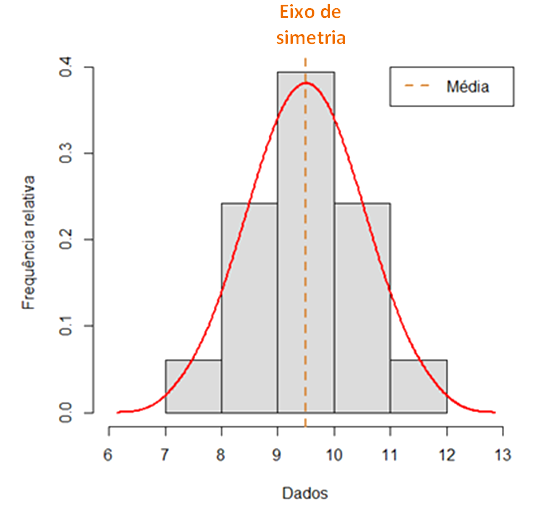
\includegraphics[scale=0.8]{assimetria1.png}
\setlength{\abovecaptionskip}{0.5pt}
\caption{Distribuição simétrica com eixo de simetria no centro}
\label{fig:distsimetrica1} % Unique label used for referencing the figure in-text
\end{figure}

Sempre que a curva da distribuição se afastar do referido eixo, será considerada como tendo um certo grau de afastamento, que é considerado como uma assimetria da distribuição. Ou seja, assimetria é o grau de afastamento que uma distribuição apresenta do seu eixo de simetria. \\

Pode-se caracterizar uma distribuição de frequência em:

\begin{itemize}
\item Distribuição simétrica (ou assimetria nula);
\item Distribuição assimétrica à direita (ou positiva);
\item Distribuição assimétrica à esquerda (ou negativa).\\
\end{itemize}


\subsubsection{Distribuição simétrica (ou assimetria nula)}
\vspace{0,1cm}

Uma distribuição é dita simétrica (Figura~\ref{fig:distsimetrica2}) quando apresenta o mesmo valor para a moda, a média e a mediana, ou seja: $\bar{x}=m_d=m_o$. \\

\begin{figure}[h!]
\centering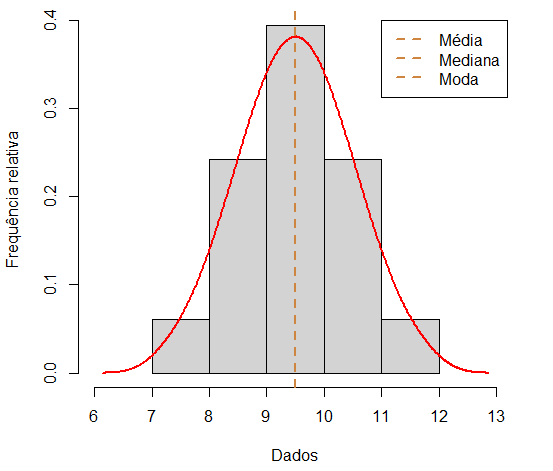
\includegraphics[scale=0.8]{assimetria2.png}
%\setlength{\abovecaptionskip}{0.5pt}
\caption{Distribuição simétrica}
\label{fig:distsimetrica2} % Unique label used for referencing the figure in-text
\end{figure}


\subsubsection{Distribuição assimétrica à direita (ou positiva)}
\vspace{0,1cm}

Quando a cauda da curva da distribuição declina para direita, tem-se uma distribuição com curva assimétrica positiva (Figura~\ref{fig:distassimetricapositiva}). Neste caso, tem-se a relação: $\bar{x}>m_d>m_o$. \\

\begin{figure}[h!]
\centering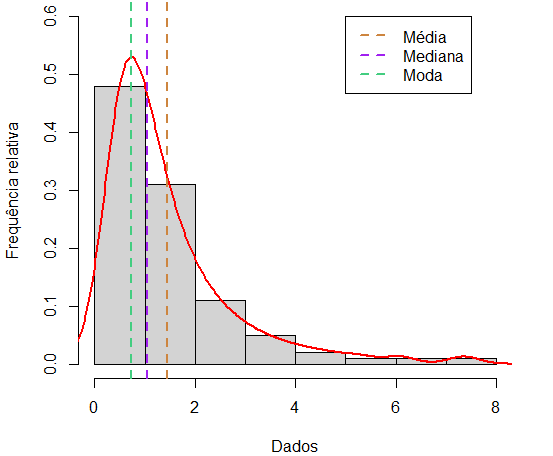
\includegraphics[scale=0.8]{assimetria3.png}
%\setlength{\abovecaptionskip}{0.5pt}
\setlength\belowcaptionskip{1cm}
\caption{Distribuição assimétrica à direita}
\label{fig:distassimetricapositiva} % Unique label used for referencing the figure in-text
\end{figure}


\subsubsection{Distribuição assimétrica à esquerda (ou negativa)}
\vspace{0,1cm}

Analogamente, quando a cauda da curva da distribuição declina para esquerda, tem-se uma distribuição com curva assimétrica negativa (Figura~\ref{fig:distassimetricanegativa}). Neste caso, tem-se a relação: $\bar{x}<m_d<m_o$. \\

\begin{figure}[h!]
\centering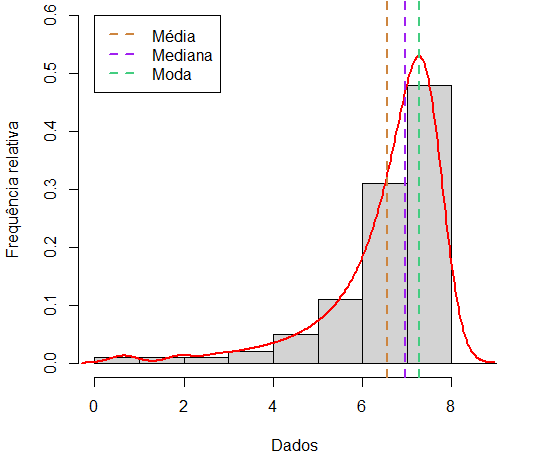
\includegraphics[scale=0.8]{assimetria4.png}
%\setlength{\abovecaptionskip}{0.5pt}
\caption{Distribuição assimétrica à esquerda}
\label{fig:distassimetricanegativa} % Unique label used for referencing the figure in-text
\end{figure}

\vspace{4cm}

\subsubsection{Coeficiente momento de assimetria}

Outra forma de verificar a assimetria de uma distribuição é por meio de um coeficiente de assimetria. Existem vários coeficientes de assimetria e, dentre eles, pode-se citar o coeficiente momento de assimetria, calculado com base nos momentos centrais de segunda e terceira ordem, definido pela Equação~\ref{eq:coefassimetriapearson}. \\

\begin{eBox}
\vspace{-0.5cm}
\begin{equation} \label{eq:coefassimetriapearson}
AS=\frac{m_3}{(\sqrt{m_2})^3} \\
\end{equation}
\end{eBox}

\noindent em que: \\

\begin{center}
$\displaystyle m_2=\frac{\displaystyle\sum_{i=1}^{n} (x_i-\bar{x})^2}{n}$ \,\,\,\, e \,\,\,\, $\displaystyle m_3=\frac{\displaystyle\sum_{i=1}^{n} (x_i-\bar{x})^3}{n}$, \\
\end{center}

\noindent para dados brutos, ou, ainda: \\

\begin{center}
$\displaystyle m_2=\frac{\displaystyle\sum_{i=1}^{n} (x_i-\bar{x})^2 f_i}{n}$ \,\,\,\, e \,\,\,\, $\displaystyle m_3=\frac{\displaystyle\sum_{i=1}^{n} (x_i-\bar{x})^3 f_i}{n}$, \\
\end{center}


\noindent se os dados estiverem agrupados em uma distribuição de frequências. \\

A interpretação do coeficiente de assimetria é: \\

\begin{itemize}
\item $AS=0$: a distribuição é simétrica;
\item $AS>0$: a distribuição é assimétrica positiva (à direita);
\item $AS<0$: a distribuição é assimétrica negativa (à esquerda). \\
\end{itemize}

\vspace{0,2cm}

\begin{example} \label{exemp:assimetria}

	Considere os dados brutos dos salários (em x sal. mín.) de 36 indivíduos:
	
	\begin{center}
	\begin{tabular}{c c c c c c c c c}
	\hline
	5,73  &  13,60  &  13,23  &  8,46  &  17,26  &  16,22  &  8,74  &  23,30  &  7,39 \\
	11,06  &  13,85  &  8,12  &  15,99  &  10,76  &  6,26  &  9,80  &  5,25  &  9,77 \\
	19,40  &  10,53  &  11,59  &  14,69  &  8,95  &  9,35  &  4,56  &  4,00  &  9,13 \\
	14,71  &  12,00  &  7,59  &  7,44  &  6,66  &  12,79  &  18,75  &  6,86  &  16,61 \\
	\hline
	\end{tabular}
	\end{center}
	
	\vspace{0,1cm}
	
	A média e a mediana dos dados brutos dos salários são, respectivamente, $\bar{x}=11,12$  e  $m_d=10,17$. Assim, tem-se a relação $\bar{x}>m_d$ e, portanto, a distribuição dos salários é assimétrica à direita. {\bf Observação}: A moda não foi apresentada neste exemplo pois para dados contínuos deve-se agrupar os dados em uma distribuição de frequências para estimar a moda. \\
	
	Para calcular o coeficiente momento de assimetria deve-se, primeiro, calcular os momentos centrais de segunda e terceira ordem: \\
	
\begin{center}
$\displaystyle m_2=\frac{\sum (x_i-\bar{x})^2}{n}=\frac{736,57}{36}=20,46$ \,\,\, e \,\,\, $\displaystyle m_3=\frac{\sum (x_i-\bar{x})^3}{n}=\frac{2.084,59}{36}=57,91$. \\
\end{center}
	
\vspace{0,2cm}
	
Portanto, o coeficiente momento de assimetria é obtido por: \\

\begin{center}
$\displaystyle AS=\frac{m_3}{(\sqrt{m_2})^3}=\frac{57,91}{(\sqrt{20,46})^3}=0,63$. \\
\end{center}

\vspace{0,2cm}

Como $AS>0$ então a distribuição dos salários é assimétrica à direita.\\	


Pode-se também observar a assimetria desta distribuição por meio de gráficos. Na Figura~\ref{fig:histboxplotsalarios} são apresentados um histograma e um boxplot dos salários nos quais fica evidente que a distribuição é assimétrica à direita. \\ 

	
	\begin{figure}[h!]
	\centering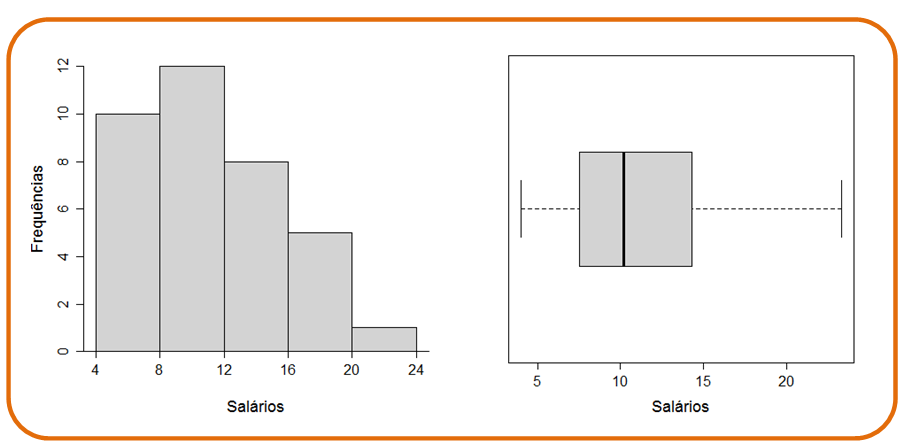
\includegraphics[scale=0.75]{assimetria5.png}
	%\setlength{\abovecaptionskip}{0.5pt}
	\caption{Histograma e boxplot dos salários}
	\label{fig:histboxplotsalarios} % Unique label used for referencing the figure in-text
	\end{figure}
	
		 
\end{example}


\vspace{0,3cm}


Na Lista~\ref{lst:Rcoefassimetria} são apresentados os comandos do software R para calcular o coeficiente momento de assimetria para os dados de salários do Exemplo~\ref{exemp:assimetria}. \\

\begin{scriptsize}
	\estiloR
	\begin{lstlisting}[caption={Comandos do software R}, label=lst:Rcoefassimetria]
	# Entrando com os dados no R
	dados <- c(5.73, 13.60, 13.23, 8.46, 17.26, 16.22, 8.74, 23.30, 7.39,
			11.06, 13.85, 8.12, 15.99, 10.76, 6.26, 9.80, 5.25, 9.77,
			19.40, 10.53, 11.59, 14.69, 8.95, 9.35, 4.56, 4.00, 9.13,
			14.71, 12.00, 7.59, 7.44, 6.66, 12.79, 18.75, 6.86, 16.61)

	# Carregando o pacote "moments" (precisa instalar)
	library(moments)
	
	# Coeficiente momento de assimetria
	skewness(dados)

	\end{lstlisting}
\end{scriptsize}







%------------------------------------------------

\section{Curtose}

A curtose é uma medida do grau de achatamento da distribuição quando comparada ao de uma distribuição conhecida como distribuição normal (que será vista na disciplina de Probabilidade). Na Figura~\ref{fig:distcurtose} pode-se obserar distribuições com diferentes graus de curtose. \\

Existem coeficientes que podem ser utilizados para determinar o grau de curtose de uma distribuição de frequências. Dentre eles pode-se citar o coeficiente momento de curtose. Este coeficiente é definido na Equação~\ref{eq:coefcurtose}, e é dado pelo quociente entre o momento centrado de quarta ordem e o quadrado do momento centrado de segunda ordem. \\

\begin{eBox}
\vspace{-0.5cm}
\begin{equation} \label{eq:coefcurtose}
k_m=\frac{m_4}{(m_2)^2} \\
\end{equation}
\end{eBox}

\noindent em que:

\begin{center}
$\displaystyle m_2=\frac{\displaystyle\sum_{i=1}^{n} (x_i-\bar{x})^2}{n}$ \,\,\,\, e \,\,\,\, $\displaystyle m_4=\frac{\displaystyle\sum_{i=1}^{n} (x_i-\bar{x})^4}{n}$, \\
\end{center}

\noindent para dados brutos, ou, ainda: \\

\begin{center}
$\displaystyle m_2=\frac{\displaystyle\sum_{i=1}^{n} (x_i-\bar{x})^2 f_i}{n}$ \,\,\,\, e \,\,\,\, $\displaystyle m_4=\frac{\displaystyle\sum_{i=1}^{n} (x_i-\bar{x})^4 f_i}{n}$, \\
\end{center}

\noindent se os dados estiverem agrupados em uma distribuição de frequências. \\

\begin{figure}[h!]
\centering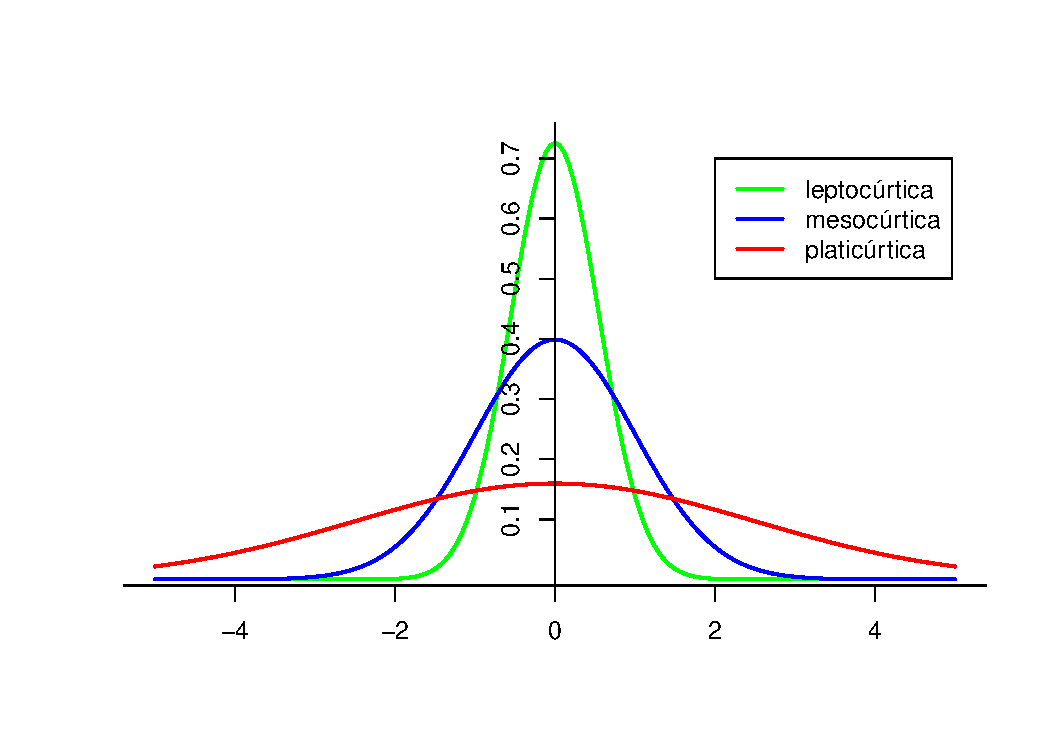
\includegraphics[trim=0 1.2cm 0 2cm, scale=0.7]{curtose1.pdf}
\setlength{\abovecaptionskip}{0.5pt}
\caption{Distribuições com diferentes graus de curtose}
\label{fig:distcurtose} % Unique label used for referencing the figure in-text
\end{figure}

\vspace{0,3cm}

Para a distribuição Normal o valor do coeficiente de curtose é 3, ou seja, é uma distribuição mesocúrtica. Coeficientes maiores que 3, representam as distribuições mais "afiladas" que a distribuição Normal, ou seja, leptocúrticas. E distribuições com coeficientes de curtose menores do que 3 representam as distribuições mais achatadas do que a Normal, ou seja, platicúrticas. Resumidamente tem-se a seguinte interpretação do coeficiente momento de curtose: \\

\begin{itemize}
\item Se $k_m<3$, a curva ou distribuição é platicúrtica;
\item Se $k_m=3$, a curva ou distribuição é mesocúrtica;
\item Se $k_m>3$, a curva ou distribuição é leptocúrtica.
\end{itemize}

\vspace{0,5cm}

\begin{example} \label{exemp:curtose}

	Considere os dados brutos das idades (em anos) de 36 indivíduos:
	
	\begin{center}
	\begin{tabular}{c c c c c c c c c}
	\hline
	21,52 & 23,11 & 40,52 & 31,70 & 36,14 & 26,98 & 31,90 & 30,88 & 35,07 \\
	17,58 & 27,82 & 31,54 & 18,99 & 24,77 & 19,70 & 29,70 & 29,41 & 31,48 \\
	25,66 & 25,34 & 20,96 & 29,63 & 30,46 & 32,31 & 35,63 & 31,69 & 32,19 \\
	24,90 & 29,35 & 39,00 & 29,26 & 27,10 & 22,61 & 31,16 & 25,32 & 20,35 \\
	\hline
	\end{tabular}
	\end{center}
	
\vspace{0,3cm}
	
%	Observe pelo histograma das idades (Figura~\ref{fig:histcurtose}) que a distribuição é aproximadamente simétrica. \\
%	
%	\begin{figure}[h!]
%	\centering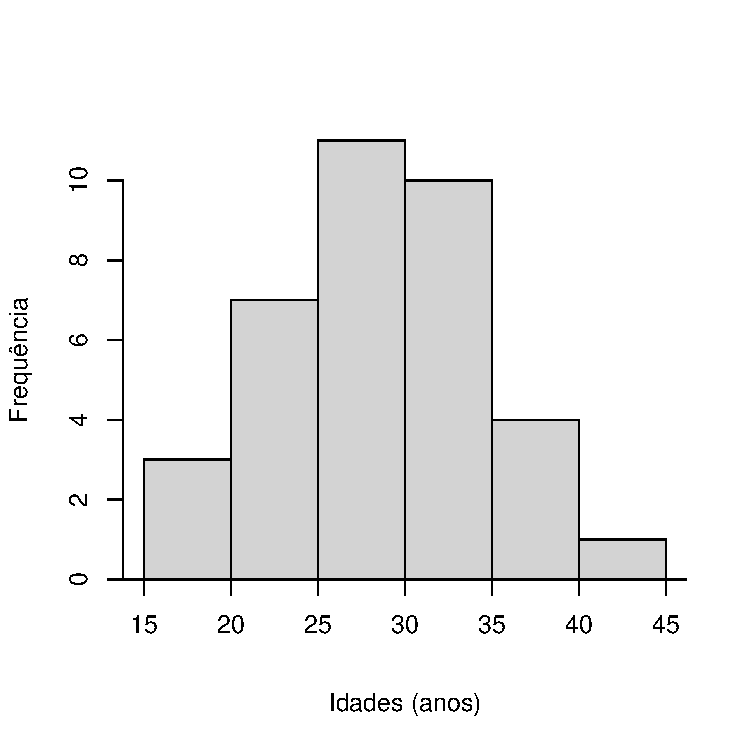
\includegraphics[trim=0 0 0 1.5cm, scale=0.75]{histcurtose.pdf}
%	\setlength{\abovecaptionskip}{0.5pt}
%	\caption{Histograma das idades}
%	\label{fig:histcurtose} % Unique label used for referencing the figure in-text
%	\end{figure}
	
	Para calcular o coeficiente momento de curtose deve-se, primeiro, calcular os momentos centrais de segunda e quarta ordem: \\
	
\begin{center}
$\displaystyle m_2=\frac{\sum (x_i-\bar{x})^2}{n}=\frac{1.088,89}{36}=30,25$ \,\,\, e \,\,\, $\displaystyle m_4=\frac{\sum (x_i-\bar{x})^4}{n}=\frac{82.885,22}{36}=2.302,37$. \\
\end{center}
	
\vspace{0,2cm}
	
Portanto, o coeficiente momento de curtose é obtido por: \\

\begin{center}
$\displaystyle k_m=\frac{m_4}{(m_2)^2}=\frac{2.302,37}{(30,25)^2}=2,52$. \\
\end{center}

\vspace{0,2cm}

Como $k_m<3$ então a distribuição dos salários é platicúrtica.\\	
		 
\end{example}

\vspace{0,3cm}


Na Lista~\ref{lst:Rcoefcurtose} são apresentados os comandos do software R para calcular o coeficiente momento de curtose para os dados de idades do Exemplo~\ref{exemp:curtose}. \\

\begin{scriptsize}
	\estiloR
	\begin{lstlisting}[caption={Comandos do software R}, label=lst:Rcoefcurtose]
	# Entrando com os dados no R
	dados <- c(21.52, 23.11, 40.52, 31.70, 36.14, 26.98, 31.90, 30.88, 35.07,
			17.58, 27.82, 31.54, 18.99, 24.77, 19.70, 29.70, 29.41, 31.48,
			25.66, 25.34, 20.96, 29.63, 30.46, 32.31, 35.63, 31.69, 32.19,
			24.90, 29.35, 39.00, 29.26, 27.10, 22.61, 31.16, 25.32, 20.35)


	# Carregando o pacote "moments" (precisa instalar)
	library(moments)
	
	# Coeficiente momento de curtose
	kurtosis(dados)

	\end{lstlisting}
\end{scriptsize}



%----------------------------------------------------------------------------------------
%	CHAPTER 10
%----------------------------------------------------------------------------------------

\chapterimage{chapter_head_3.pdf} % Chapter heading image

\chapter{Análise Bivariada}

Até agora foi visto como organizar e resumir informações pertinentes a uma única variável, mas frequentemente, existe o interesse em analisar o comportamento conjunto de duas ou mais variáveis.

%------------------------------------------------

\section{Variáveis qualitativas}

\subsection{Tabelas de contingência e gráficos da distribuição conjunta}

Tabelas de contingência são tabelas de dupla entrada que representam a distribuição conjunta de duas variáveis qualitativas. \\

\begin{example} \label{exemp:distconjinstrucaoprocedencia1}

Suponha que se queira analisar o comportamento conjunto das variáveis $X$: grau de instrução e $Y$: região de procedência de 36 indivíduos cujos dados são apresentados na Tabela~\ref{tab:instrucaoprocedencia}. \\

\begin{table}[h]
	\caption{Região de procedência e grau de instrução de 36 indivíduos}
	\label{tab:instrucaoprocedencia} 
	\vspace{-0.1cm}
	\centering
	\begin{tabular}{c c c | c c c | c c c}
	\toprule
  		&	Região & Grau	& 	&   Região	& Grau 	&	 	&	Região & Grau	 \\
  	ID	& proced. &	instrução & ID &	proced. & instrução	&	ID	& proced. &	instrução\\
  	\hline
	1	&	Capital	&	Fundamental	&	13	&	Interior	&	Médio	&	25	&	Outra	&	Fundamental	\\
	2	&	Interior	&	Fundamental	&	14	&	Capital	&	Médio	&	26	&	Outra	&	Médio	\\
	3	&	Interior	&	Médio	&	15	&	Capital	&	Médio	&	27	&	Capital	&	Fundamental	\\
	4	&	Outra	&	Fundamental	&	16	&	Outra	&	Médio	&	28	&	Outra	&	Fundamental	\\
	5	&	Interior	&	Médio	&	17	&	Interior	&	Superior	&	29	&	Outra	&	Fundamental	\\
	6	&	Outra	&	Médio	&	18	&	Interior	&	Médio	&	30	&	Capital	&	Médio	\\
	7	&	Outra	&	Fundamental	&	19	&	Interior	&	Fundamental	&	31	&	Outra	&	Médio	\\
	8	&	Capital	&	Fundamental	&	20	&	Outra	&	Médio	&	32	&	Capital	&	Médio	\\
	9	&	Outra	&	Fundamental	&	21	&	Capital	&	Superior	&	33	&	Interior	&	Médio	\\
	10	&	Capital	&	Fundamental	&	22	&	Capital	&	Superior	&	34	&	Interior	&	Médio	\\
	11	&	Interior	&	Fundamental	&	23	&	Outra	&	Superior	&	35	&	Capital	&	Médio	\\
	12	&	Interior	&	Superior	&	24	&	Interior	&	Médio	&	36	&	Outra	&	Superior	\\
	\bottomrule
	\end{tabular}
\end{table}


A distribuição de frequências conjunta das variáveis $X$ e $Y$ é obtida contando-se o número de indivíduos que se enquadram simultaneamente em um nível da variável $X$ e em um nível da variável $Y$. Por exemplo, o número de indivíduos que vem da capital e tem ensino fundamental é igual a $4$ pois quatro indivíduos se enquadram nessas duas categorias simultaneamente. Essas frequências são organizadas em uma tabela de dupla entrada (Tabela~\ref{tab:distconjinstrucaoprocedencia1}), chamada de tabela de contingência. \\

%\begin{table}[h]
%	\vspace{0,3cm}
%	\caption{Distribuição conjunta do grau de instrução $(X)$ e região de procedência $(Y)$}
%	\label{tab:distconjinstrucaoprocedencia1} 
%	\vspace{-0.1cm}
%	\centering
%	\begin{tabular}{c | c c c | c}
%	\toprule
%	 & & \textbf{$\bm{X}$} &  \\
%	 \cmidrule(lr){2-4}
%	\textbf{$\bm{Y}$} & Fundamental & Médio & Superior & Total \\
%	\midrule
%	Capital & 4 & 5 & 2 & 11 \\
%	Interior & 3 & 7 & 2 & 12 \\
%	Outra & 5 & 6 & 2 & 13 \\
%	\midrule
%	Total & 12 & 18 & 6 & 36 \\
%	\bottomrule
%	\end{tabular} \\
%\end{table}


\begin{table}[h]
	\vspace{0,3cm}
	\caption{Distribuição conjunta do grau de instrução $(X)$ e região de procedência $(Y)$}
	\label{tab:distconjinstrucaoprocedencia1} 
	\vspace{-0.1cm}
	\centering
	\begin{tabular}{c | c c c | c}
	\toprule
	\backslashbox{$\bm Y$}{$\bm X$} & \textbf{Fundamental} & \textbf{Médio} & \textbf{Superior} & \textbf{Total} \\
	\midrule
	Capital & 4 & 5 & 2 & 11 \\
	Interior & 3 & 7 & 2 & 12 \\
	Outra & 5 & 6 & 2 & 13 \\
	\midrule
	Total & 12 & 18 & 6 & 36 \\
	\bottomrule
	\end{tabular} \\
\end{table}

Observe na Tabela~\ref{tab:distconjinstrucaoprocedencia1} que a linha dos totais (valores: 12, 18 e 6) fornece a distribuição da variável $X$ e a coluna dos totais (valores: 11, 12 e 13) fornece a distribuição da variável $Y$. As distribuições assim obtidas são chamadas de distribuições marginais de $X$ e $Y$. \\

A distribuição conjunta de duas variáveis pode também ser feita graficamente. Na Figura~\ref{fig:distconjinstrucaoprocedencia1} é apresentado um gráfico de colunas da distribuição conjunta das variáveis grau de instrução $(X)$ e região de procedência $(Y)$. \\

\begin{figure}[h!]
\vspace{0,3cm}
\centering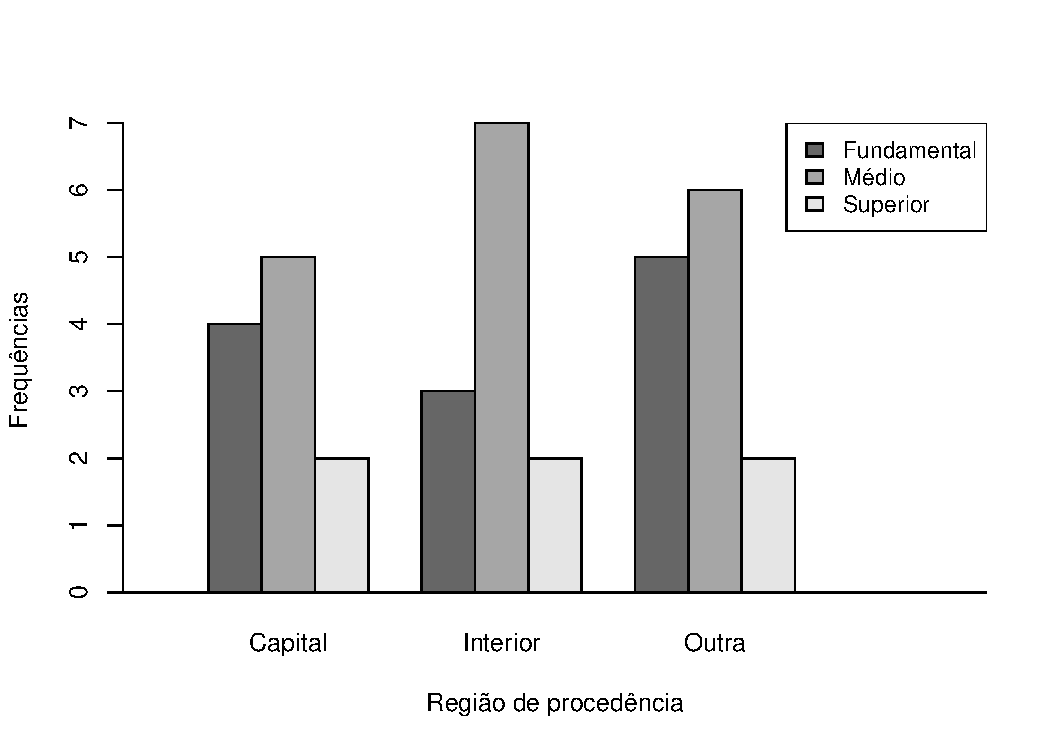
\includegraphics[trim=0 0 0 1.4cm, scale=0.7]{distconjquali1.pdf}
\setlength{\abovecaptionskip}{0.5pt}
\caption{Distribuição conjunta das frequências das variáveis grau de instrução $(X)$ e região de procedência $(Y)$}
\label{fig:distconjinstrucaoprocedencia1} % Unique label used for referencing the figure in-text
\vspace{0.5cm}
\end{figure}

\end{example}



Na Lista~\ref{lst:Rdistconjinstrucaoprocedencia1} são apresentados os comandos do software R para gerar a tabela e o gráfico da distribuição conjunta do Exemplo~\ref{exemp:distconjinstrucaoprocedencia1}.  \\


\begin{scriptsize}
	\estiloR
	\begin{lstlisting}[caption={Comandos do software R}, label=lst:Rdistconjinstrucaoprocedencia1]
	# Entrando com os dados no R
	dados <- read.table("C:caminho_do_diretorio/data6.txt",h=T)
	dados

	# Tabela de distribuição conjunta
	tabela <- table(dados$Região, dados$Instrução); tabela

	# Distribuições marginais (linha e coluna dos totais)
	addmargins(tabela)

	# Plotando o gráfico da distribuição conjunta
	barplot(t(tabela), beside=T, col=c("gray40","gray65","gray90"), 
			xlab="Região de procedência", ylab="Frequências", xlim=c(0,16))
	abline(h=0)

	# Adicionando as legendas (nomes das colunas por cores)
	legend("topright", legend=colnames(tabela), cex=0.9,
			fill=c("gray40","gray65","gray90"))
	

	\end{lstlisting}
\end{scriptsize}

\noindent {\bf Observações}: 

\noindent (a) no comando \texttt{barplot()} foi usado o argumento \texttt{t(tabela)} para transpor a matriz da distribuição conjunta de forma que as regiões de procedência fiquem nas colunas e apareçam como as categorias do gráfico de colunas; 

\noindent (b) o arquivo de dados utilizado na Lista~\ref{lst:Rdistconjinstrucaoprocedencia1}  pode ser baixado em \url{https://drive.google.com/drive/folders/1tCzWnInYGOdpC0qQsJ2EvJLDqLQ7z8aB?usp=sharing}. \\



\subsection{Associação entre Variáveis Qualitativas}

Um dos principais objetivos de se construir uma distribuição conjunta de duas variáveis qualitativas é descrever a associação entre elas, isto é, quando se quer conhecer o grau de dependência entre elas. \\

\begin{example}

Considere a distribuição conjunta do sexo e escolha do curso de 200 alunos de uma faculdade (Tabela~\ref{tab:distconjsexocurso1}). \\


\begin{table}[h]
	\caption{Distribuição conjunta de alunos segundo o sexo $(X)$ e a escolha do curso $(Y)$}
	\label{tab:distconjsexocurso1} 
	\vspace{-0.1cm}
	\centering
	\begin{tabular}{c | c c | c}
	\toprule
	\backslashbox{$\bm Y$}{$\bm X$} & \textbf{Masculino} & \textbf{Feminino} & \textbf{Total} \\
	\midrule
	Economia & 85 & 35 & 120 \\
	Administração & 55 & 25 & 80 \\
	\midrule
	Total & 140 & 60 & 200 \\
	\bottomrule
	\end{tabular} \\
\end{table}


Inicialmente é muito difícil tirar alguma conclusão sobre a existência de associação entre as duas variáveis devido à diferença entre os totais marginais. Deve-se, então, calcular as proporções ou porcentagens segundo as linhas ou segundo as colunas para que se possa fazer comparações. Calculando as porcentagens em relação aos totais das linhas obtém-se a Tabela~\ref{tab:distconjsexocurso2}. \\

\begin{table}[h]
\caption{Porcentagens em relação aos totais das linhas da distribuição conjunta do sexo $(X)$ e da escolha do curso $(Y)$}
	\label{tab:distconjsexocurso2} 
	\vspace{-0.1cm}
	\centering
	\begin{tabular}{c | r r | r}
	\toprule
	\backslashbox{$\bm Y$}{$\bm X$} & \textbf{Masculino} & \textbf{Feminino} & \textbf{Total} \\
	\midrule
	Economia & $85/120=70,8\%$ & $35/120=29,2\%$ & $120/120=100\%$ \\
	Administração & $55/80=68,8\%$ & $25/80=31,2\%$ & $80/80=100\%$ \\
	\midrule
	Total & $140/200=70,0\%$ & $60/200=30,0\%$ & $200/200=100\%$ \\
	\bottomrule
	\end{tabular} \\
\end{table}

Pode-se ver na distribuição marginal da variável sexo (linha dos totais), que é independente do curso escolhido, que 70\% dos alunos são do sexo masculino e 30\% dos alunos são  do sexo feminino. Se não houvesse dependência entre as variáveis esperaría-se as mesmas proporções de homens (70\%) e de mulheres (30\%) para cada um dos cursos escolhidos. No curso de economia as porcentagens são de 70,8\% de homens e 29,2\% de mulheres e no curso de administração as porcentagens são de 68,8\% de homens e 31,2\% de mulheres. Como as porcentagens de homens e mulheres nos dois cursos são muito próximas {\bf parece não haver dependência} entre as duas variáveis (sexo e escolha do curso). \\

Outra forma de avaliar a dependência entre duas variáveis é por meio de gráficos. Na Figura~\ref{fig:distconjsexocurso1} pode-se observar a distribuição conjuta das variáveis sexo e escolha do curso em termos das porcentagens de homens e mulheres em cada curso. Observe que como as porcentagens de homens e mulheres no curso de economia são muito parecidas com as porcentagens de homens e mulheres no curso de administração então parece que a escolha do curso independe do sexo, ou seja, {\bf parece não haver dependência} entre as variáveis sexo e escolha do curso.


\begin{figure}[h!]
\vspace{0,3cm}
\centering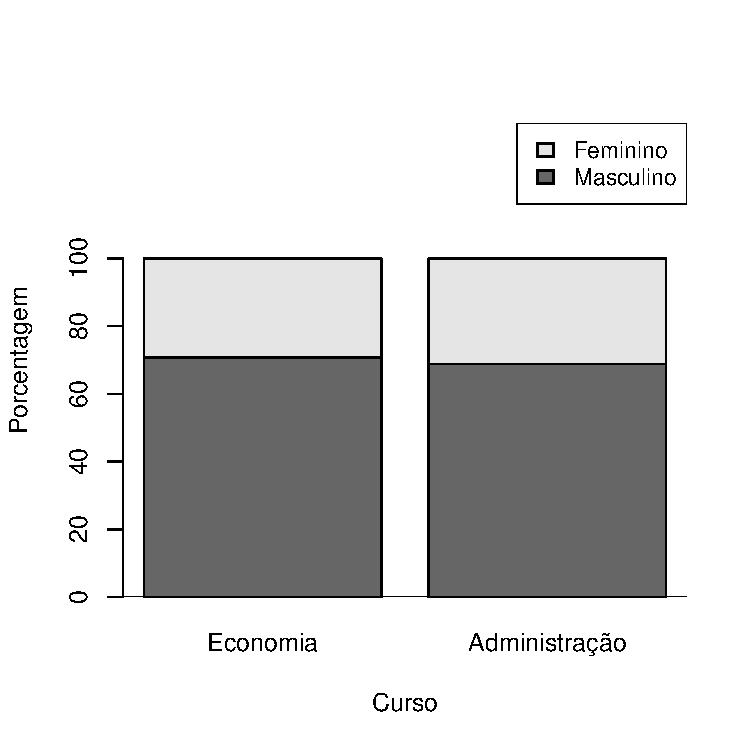
\includegraphics[trim=0 0 0 1.4cm, scale=0.7]{distconjquali2.pdf}
\setlength{\abovecaptionskip}{0.5pt}
\caption{Distribuição conjunta do sexo $(X)$ e da escolha do curso $(Y)$}
\label{fig:distconjsexocurso1} % Unique label used for referencing the figure in-text
\vspace{0.5cm}
\end{figure}


\end{example}



\vspace{1cm}

\begin{example} \label{exemp:distconjsexo}

Considere, agora, um problema semelhante ao do exemplo anterior, porém envolvendo alunos dos cursos de Física e Ciências Sociais. A distribuição conjunta das variáveis sexo e escolha do curso são apresentadas na Tabela~\ref{tab:distconjsexocurso3}.\\

\begin{table}[h]
\caption{Porcentagens em relação aos totais das linhas da distribuição conjunta do sexo $(X)$ e da escolha do curso $(Y)$}
	\label{tab:distconjsexocurso3} 
	\vspace{-0.1cm}
	\centering
	\begin{tabular}{c | c c | c}
	\toprule
	\backslashbox{$\bm Y$}{$\bm X$} & \textbf{Masculino} & \textbf{Feminino} & \textbf{Total} \\
	\midrule
	Física & $100$ & $20$ & $120$ \\
	Ciências sociais & $40$ & $40$ & $80$ \\
	\midrule
	Total & $140$ & $60$ & $200$ \\
	\bottomrule
	\end{tabular} \\
\end{table}

Calculando as porcentagens segundo os totais das linhas obtém-se a Tabela~\ref{tab:distconjsexocurso4}. \\


\begin{table}[h]
\caption{Porcentagens, segundo os totais das linhas, da distribuição conjunta do sexo $(X)$ e do curso escolhido $(Y)$.}
	\label{tab:distconjsexocurso4} 
	\vspace{-0.1cm}
	\centering
	\begin{tabular}{c | r r | r}
	\toprule
	\backslashbox{$\bm Y$}{$\bm X$} & \textbf{Masculino} & \textbf{Feminino} & \textbf{Total} \\
	\midrule
	Física & $100/120=83,3\%$ & $20/120=16,7\%$ & $120/120=100\%$ \\
	Ciências sociais & $40/80=50,0\%$ & $40/80=50,0\%$ & $80/80=100\%$ \\
	\midrule
	Total & $140/200=70,0\%$ & $60/200=30,0\%$ & $200/200=100\%$ \\
	\bottomrule
	\end{tabular} \\
\end{table}


Pode-se ver que no curso de Física as porcentagens são de 83,3\% de homens e 16,7\% de mulheres e no curso de Ciências sociais as porcentagens são de 50,0\% de homens e 50,0\% de mulheres.  Pode-se observar também pela Figura~\ref{fig:distconjsexocurso2} que as porcentagens de homens e mulheres no curso de Física são muito diferentes das porcentagens de homens e mulheres no curso de Ciências sociais, ou seja, {\bf parece haver dependência} entre as duas variáveis.


\end{example}

\vspace{0,3cm}

Na Lista~\ref{lst:Rdistconjsexocurso} são apresentados os comandos do software R para obter as porcentagens segundo os totais das linhas e o gráfico da distribuição conjunta em termos das porcentagens de homens e mulheres em cada curso.\\

\begin{scriptsize}
	\estiloR
	\begin{lstlisting}[caption={Comandos do software R}, label=lst:Rdistconjsexocurso]
	# Entrando com a tabela da distribuição conjunta no R
	tabela <- matrix(c(100,20,40,40), 2, 2, byrow=T)
	rownames(tabela) <- c("Física", "Ciências sociais")
	colnames(tabela) <- c("Masculino", "Feminino")
	tabela

	# Adicionando a linha dos totais
	tabela2 <- addmargins(tabela,1)
	tabela2

	# Tabela de proporções (em porcentagens)
	tabprop <- round(prop.table(tabela2,1)*100, 1)
	tabprop

	# Coluna dos totais das porcentagens
	addmargins(tabprop,2)
	tabprop <- tabprop[-3,]

	# Plotando o gráfico da distribuição conjunta
	barplot(t(tabprop), xlab="Curso", ylab="Porcentagem", axes=F, 
			ylim=c(0,140), col=c("gray40","gray90"))
	axis(2, at=seq(0,100,20)); abline(h=0)
	
	# Adicionando as legendas (nomes das colunas por cores)
	legend("topright", legend=rev(colnames(tabela2)), cex=0.9,
			fill=rev(c("gray40","gray90")))

	
	\end{lstlisting}
\end{scriptsize}

\noindent {\bf Observação}: Dentro do comando \texttt{legend()}, nos argumentos \texttt{legend} e \texttt{fill}, foi utilizado o comando \texttt{rev} para inverter a ordem dos nomes e das cores da legenda, de modo que o sexo feminino fosse apresentado primeiro do que o sexo masculino na legenda. \\

\begin{figure}[h!]
\vspace{0,3cm}
\centering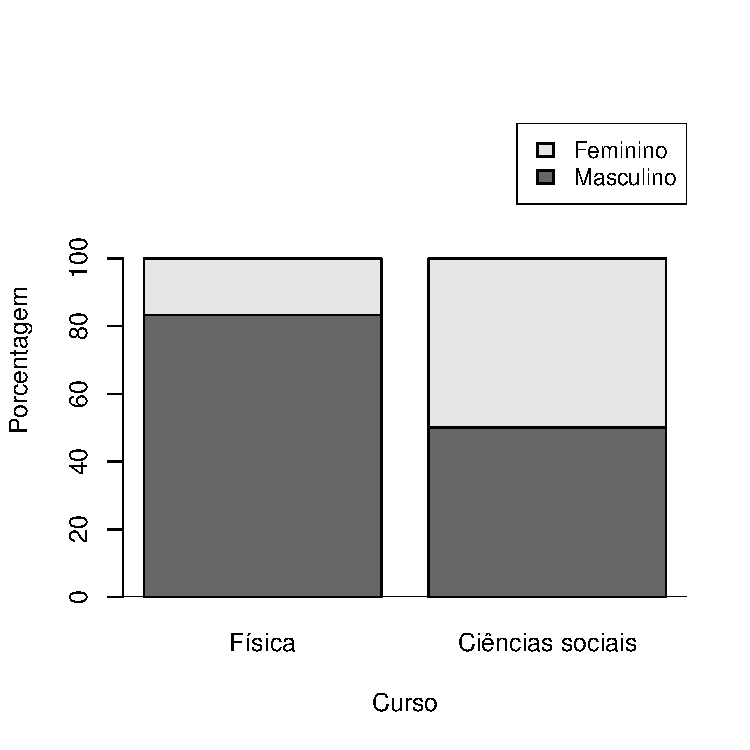
\includegraphics[trim=0 0 0 1.4cm, scale=0.7]{distconjquali3.pdf}
\setlength{\abovecaptionskip}{0.5pt}
\caption{Distribuição conjunta do sexo $(X)$ e da escolha do curso $(Y)$}
\label{fig:distconjsexocurso2} % Unique label used for referencing the figure in-text
\vspace{0.5cm}
\end{figure}


\subsection{Qui-quadrado $(\chi^2)$}

\vspace{0,3cm}

Define-se o Qui-quadrado de Pearson pela Equação~\ref{eq:quiquadrado}. \\

\begin{eBox}
\vspace{-0.5cm}
\begin{equation} \label{eq:quiquadrado}
\displaystyle \sum_{i=1}^r \sum_{j=1}^s \frac{(o_{ij}-e_{ij})^2}{e_{ij}} \\
\end{equation}
\end{eBox}

\noindent em que:

\begin{itemize}
\item $r$ é o número de linhas da tabela de contingência;
\item $s$ é o número de colunas da tabela de contingência;
\item $o_{ij}$ são as frequências observadas na distribuição conjunta;
\item $e_{ij}$ são as frequências esperadas, ou seja, valores esperados das frequências caso não existisse associação entre as variáveis. O cálculo das frequências esperadas é feito por: \\

\begin{center}
$\displaystyle e_{ij}=\frac{(\textrm{Total da linha } i)\times(\textrm{Total da coluna } j)}{\textrm{Total de observações}}.$
\end{center}

\end{itemize}

O qui-quadrado é uma medida de afastamento global entre as frequências observadas e esperadas e quanto maior seu valor maior é o grau de associação entre as variáveis. \\


\begin{example} \label{exemp:quiquadrado}

Considere a distribuição conjunta do sexo e da escolha do curso apresentada no Exemplo~\ref{exemp:distconjsexo} (Tabela~\ref{tab:distconjsexocurso3}). \\

\begin{table}[h]
	\begin{rBox}
	\captionsetup{labelformat=empty}
	\caption{\color{olivine!130}{Recordando a Tabela~\ref{tab:distconjsexocurso3}}}
	\centering
	{\color{olivine!130} 
	\begin{tabular}{c | c c | c}
	\toprule
	\backslashbox{$\bm Y$}{$\bm X$} & \textbf{Masculino} & \textbf{Feminino} & \textbf{Total} \\
	\midrule
	Física & $100$ & $20$ & $120$ \\
	Ciências sociais & $40$ & $40$ & $80$ \\
	\midrule
	Total & $140$ & $60$ & $200$ \\
	\bottomrule
	\end{tabular}} \\
	\end{rBox}
\end{table}

As frequências no interior da Tabela~\ref{tab:distconjsexocurso3} são as frequências observadas. As frequências esperadas são calculadas por: \\

\begin{center}
\begin{tabular}{c | c}
\midrule
$\displaystyle e_{11}=\frac{120 \times 140}{200}=84$ & $\displaystyle e_{12}=\frac{120 \times 60}{200}=36$ \\
\midrule
$\displaystyle e_{21}=\frac{80 \times 140}{200}=56$ & $\displaystyle e_{22}=\frac{80 \times 60}{200}=24$ \\
\midrule
\end{tabular}
\end{center}

\vspace{0,3cm}

Na Tabela~\ref{tab:quiquadrado} são apresentadas as frequências observadas $(o_{ij})$ e esperadas $(e_{ij})$ segundo o sexo $(X)$ e a escolha do curso $(Y)$. \\


\begin{table}[h]
\caption{Frequências observadas $(o_{ij})$ e esperadas $(e_{ij})$ segundo o sexo $(X)$ e a escolha do curso $(Y)$}
	\label{tab:quiquadrado} 
	\vspace{-0.1cm}
	\centering
	\begin{tabular}{c | c c | c}
	\toprule
	\backslashbox{$\bm Y$}{$\bm X$} & \textbf{Masculino} & \textbf{Feminino} & \textbf{Total} \\
	\midrule
	Física & $100$ \textcolor{ocre}{$(84)$} & $20$ \textcolor{ocre}{$(36)$} & $120$ \\
	Ciências sociais & $40$ \textcolor{ocre}{$(56)$} & $40$ \textcolor{ocre}{$(24)$} & $80$ \\
	\midrule
	Total & $140$ & $60$ & $200$ \\
	\bottomrule
	\end{tabular} \\
\end{table}

Portanto o qui-quadrado é calculado como: \\

\begin{center}
$\displaystyle \sum_{i=1}^r \sum_{j=1}^s \frac{(o_{ij}-e_{ij})^2}{e_{ij}}
= \frac{(100-84)^2}{84} + \frac{(20-36)^2}{36}
+ \frac{(40-56)^2}{56} + \frac{(40-24)^2}{24} 
= 25,4$. \\
\end{center}


\end{example}



\subsection{Coeficiente de contingência}

Pearson definiu, ainda, uma medida de associação baseada no qui-quadrado, chamada de coeficiente de contingência (de Pearson), dado pela Equação~\ref{eq:coefcontingencia1}. \\

\begin{eBox}
\vspace{-0.5cm}
\begin{equation} \label{eq:coefcontingencia1}
\displaystyle C=\sqrt{\frac{\chi^2}{\chi^2+n}}. \\
\end{equation}
\end{eBox}

\vspace{0,2cm}

Quanto mais próximo de zero o valor de $C$ estiver, menor será a associação entre as variáveis $X$ e $Y$ e quanto mais próximo de um o valor de $C$ estiver, maior será a associação entre as duas variáveis. Contudo, o coeficiente acima nunca atinge o valor $1$. O valor máximo de $C$ depende de $r$ e $s$ (número de linhas e colunas, respectivamente). Para evitar esse inconveniente, costuma-se definir um outro coeficiente de contingência (de Tschuprow), que é um coeficiente de contingência corrigido, dado pela Equação~\ref{eq:coefcontingencia2}. \\

\begin{eBox}
\vspace{-0.5cm}
\begin{equation} \label{eq:coefcontingencia2}
\displaystyle T=\sqrt{\frac{\chi^2/n}{\sqrt{(r-1)(s-1)}}}, \\
\end{equation}
\end{eBox}

\vspace{0,2cm}

\noindent que pode atingir o máximo igual a $1$ se $r=s$ (número de linhas tabela igual ao número de colunas).

\vspace{0,3cm}

\begin{example}

Considere o Exemplo~\ref{exemp:quiquadrado}. O valor obtido do qui-quadrado foi $\chi^2=25,4$. Os coeficientes de contingência são calculados por: 

\begin{center}
$\displaystyle C=\sqrt{\frac{\chi^2}{\chi^2+n}}=\sqrt{\frac{25,4}{25,4+200}}=0,336$, \\
\end{center}

e

\begin{center}
$\displaystyle T=\sqrt{\frac{\chi^2/n}{\sqrt{(r-1)(s-1)}}}=\sqrt{\frac{25,4/200}{\sqrt{(2-1)(2-1)}}}=0,3563$. \\
\end{center}

indicando uma associação "moderada" entre as variáveis sexo $(X)$ e escolha do curso $(Y)$. 

\end{example}

\vspace{0,3cm}

Na Lista~\ref{lst:Rcoefcontingencia} são apresentados os comandos do software R para obter o coeficiente de contingência.\\

\begin{scriptsize}
	\estiloR
	\begin{lstlisting}[caption={Comandos do software R}, label=lst:Rcoefcontingencia]
	# Entrando com a distribuição conjunta no R
	tabela <- matrix(c(100, 20, 40, 40), 2, 2, byrow=T)
	
	# Adicionando os nomes das linhas e colunas
	rownames(tabela) <- c("Física", "Ciências sociais")
	colnames(tabela) <- c("Masculino", "Feminino")
	tabela

	# Qui-quadrado usando o comando "chisq.test()"
	chisq.test(tabela,correct=FALSE)
	
	# Carregando o pacote vcd (precisa instalar)
	library(vcd)
	
	# Diversos qui-quadrados e coeficientes de contingência
	assocstats(tabela)

	# Qui-quadrado de Pearson
	X2 <- assocstats(tabela)[[2]][2,1]; X2

	# Coeficiente de contingência de Pearson (C)
	C <- assocstats(tabela)[[4]]; C
	
	# Coeficiente de contingência de Tschuprow (T)
	n <- sum(tabela)
	r <- nrow(tabela)
	s <- ncol(tabela)
	T <- sqrt((X2/n)/sqrt((r-1)*(s-1))); T

	
	\end{lstlisting}
\end{scriptsize}

\noindent {\bf Observação}: No comando \texttt{chisq.test()} usou-se o argumento \texttt{correct=FALSE} para que não fosse utilizada a correção de Yates para o teste Qui-quadrado em tabelas $2 \times 2$. Como, nesta disciplina, ainda não estão sendo considerados aspectos referentes à distribuição de probabilidades de estatísticas, que é o motivo pelo qual a correção de Yates é aplicada, optou-se por não utilizar esta correção no cálculo do $\chi^2$. \\



%------------------------------------------------

\section{Variáveis quantitativas}

\subsection{Gráfico de dispersão}

Um recurso bastante útil para se verificar a associação entre duas variáveis quantitativas é o gráfico de dispersão, que será introduzido por meio de exemplos. \\

\begin{example}\label{exemp:anbidvarquanti1}

Na Tabela~\ref{tab:anbidvarquanti1} são apresentados o tempo de serviço $(X)$, em anos, e o número de clientes $(Y)$ de agentes de uma companhia de seguros. \\

\begin{table}[h]
	\caption{Anos de serviço $(X)$ e o número de clientes $(Y)$ de agentes de uma companhia de seguros}
	\label{tab:anbidvarquanti1} 
	\vspace{-0.1cm}
	\centering
	\begin{tabular}{c c c}
	\toprule
	\textbf{ID do agente} & \textbf{Anos de serviço $ \bm{(X)}$} & \textbf{Número de clientes $\bm{(Y)}$} \\
	\midrule
	1 & 2 & 48 \\
	2 & 3 & 50 \\
	3 & 4 & 56 \\
	4 & 5 & 52 \\
	5 & 4 & 43 \\
	6 & 6 & 60 \\
	7 & 7 & 62 \\
	8 & 8 & 58 \\
	9 & 8 & 64 \\
	10 & 10 & 72 \\	
	\bottomrule
	\end{tabular} \\
\end{table}


Na Figura~\ref{fig:anbidvarquanti1} é apresentado o gráfico de dispersão das variáveis $X$ e $Y$. Nesse tipo de gráfico são apresentados os pares $(x,y)$ em um plano cartesiano. \\

\begin{figure}[h!]
\centering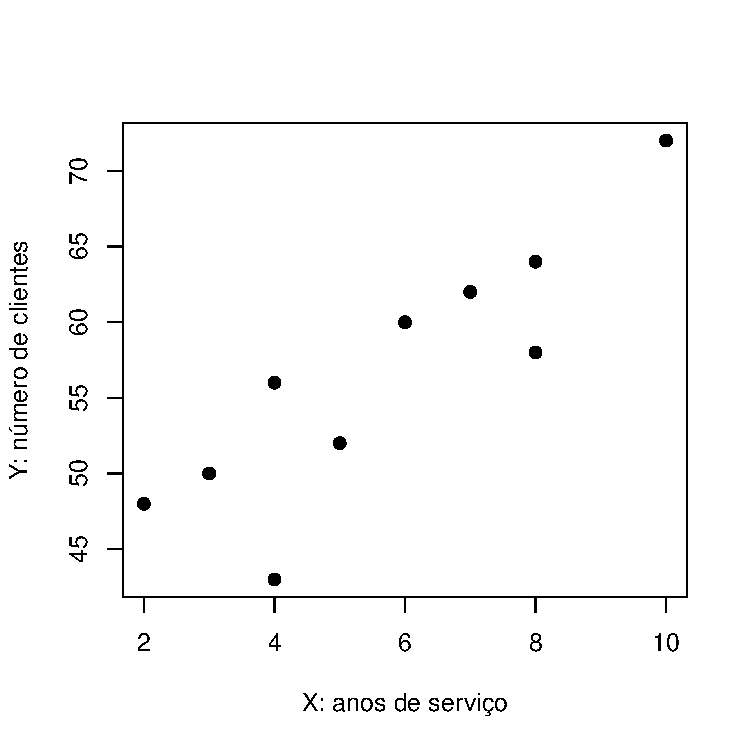
\includegraphics[trim=0 0 0 2cm, scale=0.7]{anbidvarquanti1.pdf}
\setlength{\abovecaptionskip}{0.5pt}
\caption{Gráfico de dispersão das variáveis $X$: anos de serviço e $Y$: número de clientes}
\label{fig:anbidvarquanti1} % Unique label used for referencing the figure in-text
\vspace{0.5cm}
\end{figure}

Pode-se observar por este gráfico que parece haver uma associação entre as duas variáveis porque à medida que aumenta o tempo de serviço o número de clientes também aumenta, e essa relação parece ocorrer de forma linear. 

\end{example}

\vspace{4cm}

Na Lista~\ref{lst:Ranbidvarquanti2} são apresentados os comandos do software R para obter o gráfico de dispersão $X$ versus $Y$.\\

\begin{scriptsize}
	\estiloR
	\begin{lstlisting}[caption={Comandos do software R}, label=lst:Ranbidvarquanti2]
	# Entrando com os dados no R
	X <- c(2, 3, 4, 5, 4, 6, 7, 8, 8, 10)
	Y <- c(48, 50, 56, 52, 43, 60, 62, 58, 64, 72)
	
	# Gráfico de dispersão X versus Y
	plot(X, Y, pch=19, xlab="X: tempo de serviço, em anos", 
			ylab="Y: número de clientes")

	\end{lstlisting}
\end{scriptsize}


Na Figura~\ref{fig:anbidvarquanti2} pode-se observar possíveis tipos de associação (correlação) linear entre as variáveis. Na Figura~\ref{fig:anbidvarquanti2}(a) existe uma associação linear positiva, ou seja, ao passo que uma variável aumenta a outra também aumenta. Na Figura~\ref{fig:anbidvarquanti2}(b) existe uma associação linear negativa, ou seja, ao passo que uma variável aumenta a outra variável diminui. Finalmente, na Figura~\ref{fig:anbidvarquanti2}(c) as variáveis não tem nenhuma associação linear, ou seja, quando uma variável aumenta a outra variável não aumenta e nem diminui linearmente. \\


\begin{figure}[h!]
\centering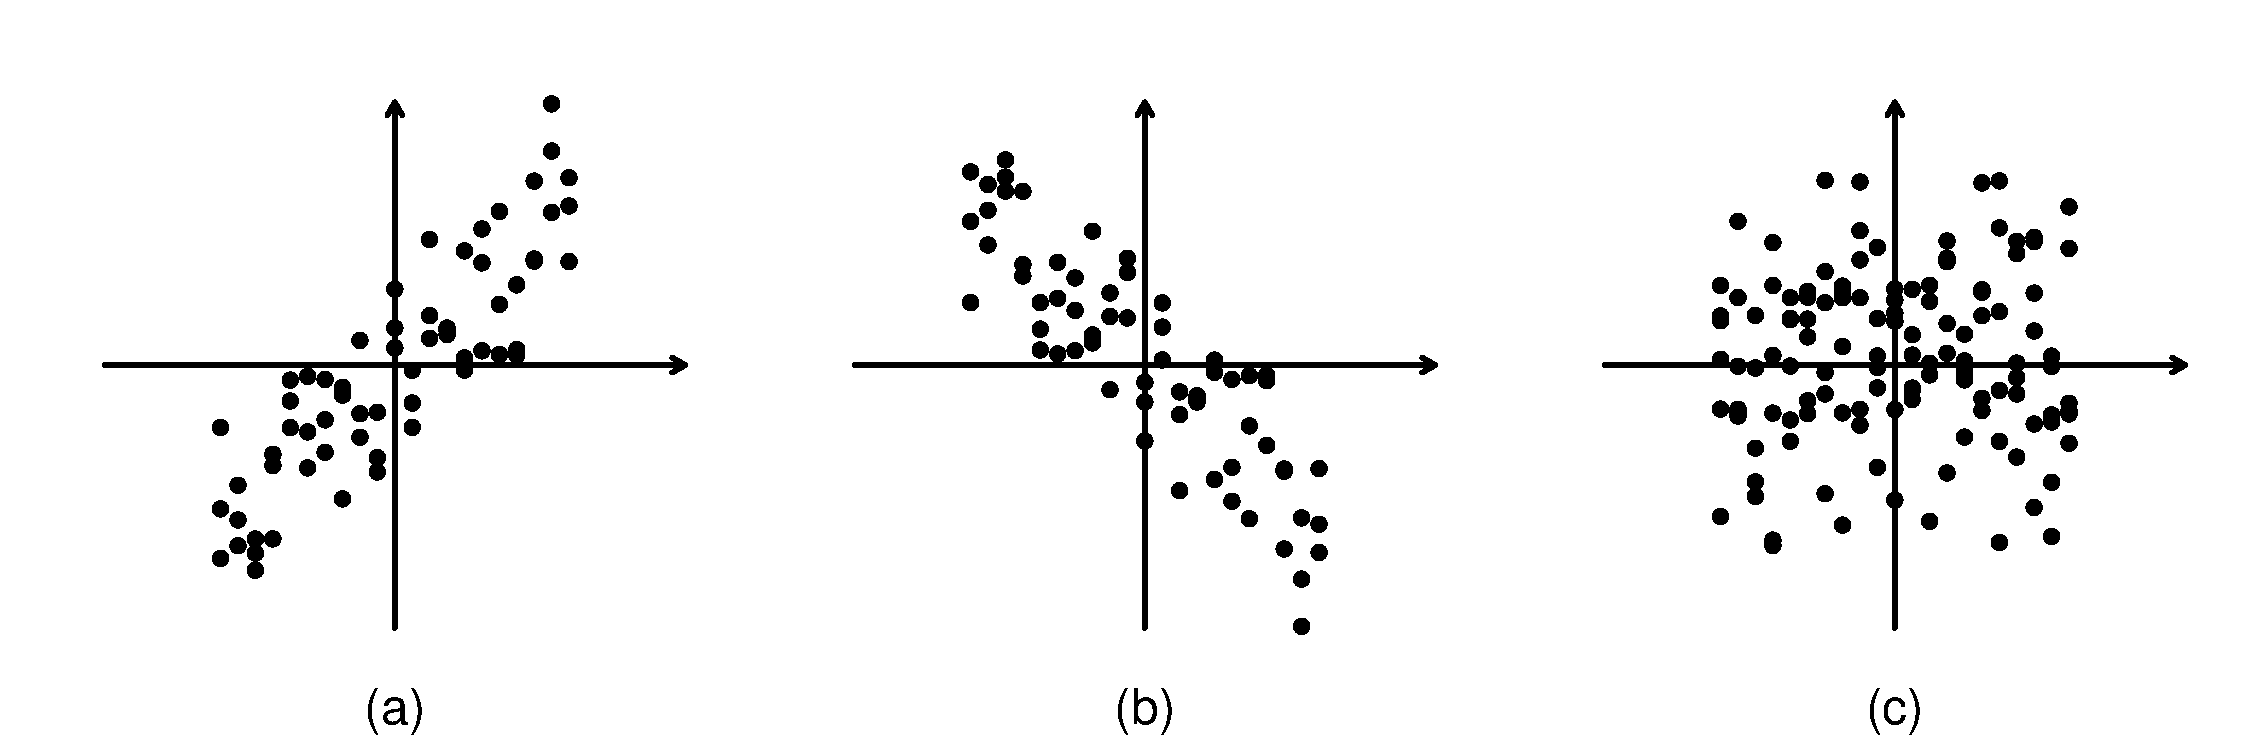
\includegraphics[trim=0 0 0 2cm, scale=0.4]{anbidvarquanti2.pdf}
\setlength{\abovecaptionskip}{0.5pt}
\caption{Tipos de associação linear entre duas variáveis quantitativas}
\label{fig:anbidvarquanti2} % Unique label used for referencing the figure in-text
\vspace{0.5cm}
\end{figure}


Quanto mais próximos de uma reta os pontos do diagrama de dispersão estiverem mais forte será a correlação entre as duas variáveis e quanto mais dispersos os pontos estiverem mais fraca será a correlação entre as duas variáveis. Pode-se determinar o grau de correlação entre duas variáveis utilizando-se, para isso, uma medida. \\



\subsection{Coeficiente de correlação}

Antes de se definir o coeficiente de correlação deve-se, primeiro, definir a covariância. A covariância é uma medida do grau de interdependência de duas variáveis quantitativas e é calculada pela Equação~\ref{eq:covariancia}. \\

\begin{eBox}
\vspace{-0.5cm}
\begin{equation} \label{eq:covariancia}
\displaystyle cov(X,Y)=\frac{\displaystyle \sum_{i=1}^{n}{(x_i-\bar{x})(y_i-\bar{y})}}{n-1} \\
\end{equation}
\end{eBox}

\vspace{0,2cm}
A covariância é uma medida diretamente afetada pela escala de mensuração das variáveis e pode variar entre $-\infty$ \, e \, $+\infty$, ou seja, $-\infty \leq cov(X,Y) \leq +\infty$. \\

Uma outra maneira de avaliar o grau de associação entre duas variáveis quantitativas é padronizando a covariância, divindo esta medida pelo produto dos desvios padrões das variáveis sob análise, denomiada de coeficiente de correlção. O coeficiente de correlação (linear) é uma medida do grau de associação (correlação) entre duas variáveis quantitativas e não é afetado pela escala de mensuração das variáveis. \\

\subsubsection{Definição}
Dados $n$ pares de valores $(x_1, y_1), \, (x_2, y_2), \, ..., (x_n, y_n)$ de duas variáveis quantitativas $X$ e $Y$, define-se o coeficiente de correlação entre $X$ e $Y$ pela Equação~\ref{eq:coefcorrelacao1}. \\

\begin{eBox}
\vspace{-0.5cm}
\begin{equation} \label{eq:coefcorrelacao1}
\displaystyle r=cor(X,Y)=\frac{cov(X,Y)}{dp(X).dp(Y)} \\
\end{equation}
\end{eBox}

\vspace{0,2cm}
\noindent em que $dp(X)$ é o desvio padrão de $X$ e $dp(Y)$ é o desvio padrão de $Y$. O coeficiente de correlação pode variar de $-1$ a $1$, ou seja: $-1 \leq r \leq 1$. \\

Um coeficiente de correlação positivo indica uma associação linear positiva entre as duas variáveis, um coeficiente de correlação negativo indica uma associação linear negativa, já um coeficiente de correlação nulo (igual a zero) indica que não existe associação linear entre as duas variáveis. Quanto mais próximo de $1$ o coeficiente de correlação estiver, mais forte é o grau de associação linear positiva entre $X$ e $Y$, e, quanto mais próximo de $-1$ o coeficiente de correlação estiver, mais forte é o grau de associação linear negativa entre $X$ e $Y$. \\

A Equação~\ref{eq:coefcorrelacao1} pode ser operacionalizada de modo mais conveniente pela Equação~\ref{eq:coefcorrelacao2}. \\


\begin{eBox}
\vspace{-0.5cm}
\begin{equation} \label{eq:coefcorrelacao2}
\displaystyle r=\frac{\displaystyle\sum_{i=1}^{n}{x_i y_i}-n\bar{x}\bar{y}}
	 {\sqrt{\left(\displaystyle\sum_{i=1}^{n}{x_i^2}-n\bar{x}^2\right)
			\left(\displaystyle\sum_{i=1}^{n}{y_i^2}-n\bar{y}^2\right)}} \\
\end{equation}
\end{eBox}

\vspace{0,2cm}

\begin{example}

Considere os dados apresentados no Exemplo~\ref{exemp:anbidvarquanti1} (Tabela~\ref{tab:anbidvarquanti1}). Para calcular o coeficiente de correlação construir uma tabela de cálculos auxiliares (Tabela~\ref{tab:anbidvarquanti2}).

\begin{table}[h]
	\caption{Tabela de cálculos auxiliares}
	\label{tab:anbidvarquanti2} 
	\vspace{-0.1cm}
	\centering
	\begin{tabular}{c c c c c c}
	\toprule
	\textbf{ID} & \textbf{$\bm{(X)}$} & \textbf{$\bm{(Y)}$} & \textbf{$\bm{(X^2)}$} & \textbf{$\bm{(Y^2)}$} & 
	\textbf{$\bm{(XY)}$}\\
	\midrule
	1 & 2 & 48 & 4 & 2304 & 96 \\
	2 & 3 & 50 & 9 & 2500 & 150 \\
	3 & 4 & 56 & 16 & 3136 & 224 \\
	4 & 5 & 52 & 25 & 2704 & 260 \\
	5 & 4 & 43 & 16 & 1849 & 172 \\
	6 & 6 & 60 & 36 & 3600 & 360 \\
	7 & 7 & 62 & 49 & 3844 & 434 \\
	8 & 8 & 58 & 64 & 3364 & 464 \\
	9 & 8 & 64 & 64 & 4096 & 512 \\
	10 & 10 & 72 & 100 & 5184 & 720 \\
	\midrule
	Total & 57 & 565 & 383 & 32.581 & 3.392 \\
	\bottomrule
	\end{tabular} \\
\end{table}

Assim, tem-se: \,\, $n=10$, \,\, $\bar{x}=5,7$, \,\, $\bar{y}=56,5$, \,\, $\sum x_i^2=383$, \,\, $\sum y_i^2=32.581$ \,\, e \,\, $\sum x_i y_i=3.392$. \\

Logo,

\begin{ceqn}
\begin{align*}
r
&= \displaystyle \frac{\displaystyle\sum_{i=1}^{n}{x_i y_i}-n\bar{x}\bar{y}}
	 {\sqrt{\left(\displaystyle\sum_{i=1}^{n}{x_i^2}-n\bar{x}^2\right)
			\left(\displaystyle\sum_{i=1}^{n}{y_i^2}-n\bar{y}^2\right)}} \\ \\
&= \displaystyle \frac{3.392 - 10 \times 5,7 \times 56,5}
	 {\sqrt{\left( 383 - 10 \times 5,7^2 \right)
			\left( 32.581 - 10 \times 56,5^2 \right)}} \\ \\
&= 0,8768.
\end{align*}
\end{ceqn}


Como o coeficiente de correlação foi próximo de $1$, significa que existe uma forte correlação linear positiva entre o tempo de serviço $(X)$ e o número de clientes $(Y)$ dos agentes da companhia de seguros. \\

\end{example}

\vspace{0,3cm}

Na Lista~\ref{lst:Ranbidvarquanti2} são apresentados os comandos do software R para obter o gráfico de dispersão $X$ versus $Y$, a covariância de $X$ e $Y$ e o coeficiente de correlação.\\

\begin{scriptsize}
	\estiloR
	\begin{lstlisting}[caption={Comandos do software R}, label=lst:Ranbidvarquanti2]
	# Entrando com os dados no R
	X <- c(2, 3, 4, 5, 4, 6, 7, 8, 8, 10)
	Y <- c(48, 50, 56, 52, 43, 60, 62, 58, 64, 72)
	
	# Gráfico de dispersão X versus Y
	plot(X, Y, pch=19, xlab="X: tempo de serviço, em anos", 
			ylab="Y: número de clientes")
			
	# Covariância
	cov(X,Y)

	# Coeficiente de correlação
	cor(X,Y)

	
	\end{lstlisting}
\end{scriptsize}



%----------------------------------------------------------------------------------------
%	BIBLIOGRAPHY
%----------------------------------------------------------------------------------------
\chapterimage{chapter_head_1.pdf} % Chapter heading image

\chapter*{Bibliografia}
\addcontentsline{toc}{chapter}{\textcolor{ocre}{Bibliografia}} % Add a Bibliography heading to the table of contents


\noindent BUSSAB, W. O., MORETTIN, P. A. {\bf Estatística Básica}. 5. ed. São Paulo: Saraiva, 2002. \\

\noindent COSTA, S. C. {\bf Estatística Aplicada à Veterinária}. Londrina: UEL, [ca. 2012]. (Notas de aula). \\

\noindent FERREIRA, D. F. {\bf Estatística Básica}. Lavras: Editora UFLA, 2005. \\

\noindent FONSECA, J. S., MARTINS, G. A.  {\bf Curso de estatística}. 6. ed. São Paulo: Atlas, 1996. \\

\noindent MELLO, M. P., PETERNELLI, L. A. {\bf Conhecendo o R: uma visão mais que Estatística}. Viçosa: Editora UFV, 2013. \\

\noindent MONTGOMERY, D. C., RUNGER, G. C. {\bf Estatística Aplicada e Probabilidade para Engenheiros}. 5. ed. Rio de Janeiro: LTC, 2012. \\

\noindent R DEVELOPMENT CORE TEAM (2020). {\bf R: A language and environment for statistical computing}. R Foundation for Statistical Computing, Vienna, Austria. URL \url{http://www.R-project.org}. \\

\noindent RIBEIRO JUNIOR, P. J. {\bf Introdução ao Ambiente Estatístico R}. Curitiba: UFPR, 2011. (Notas de aula).\\

\noindent RSTUDIO TEAM (2020). {\bf RStudio: Integrated Development for R}. RStudio, Inc., Boston, MA URL \url{http://www.rstudio.com/}. \\

\noindent VIEIRA, S. {\bf Introdução à Bioestatística}. 3. ed. rev. Rio de Janeiro: Campus, 1998.



%----------------------------------------------------------------------------------------

\end{document}
